% !TeX program = xelatex
% !TeX encoding = UTF-8
% 已接入审核中的第一至第五章初稿；未完成章节不冒充正式正文。
\documentclass[fontset=fandol,type=master,campus=harbin]{hithesisbook}
\usepackage{hithesis}
\graphicspath{{figures/}{figures/framework/}{figures/network/}{figures/experiments/}}
\begin{document}
\frontmatter
% !TeX root = ../thesis.tex
% 所有身份、学位、日期信息必须由本人及学院核实后填写。
\hitsetup{
  statesecrets={待确认},
  natclassifiedindex={待填写},
  intclassifiedindex={待填写},
  ctitlecover={面向灵巧手触觉信号的仿真到现实迁移方法研究},
  ctitle={面向灵巧手触觉信号的仿真到现实迁移方法研究},
  cxueke={待确认学位类别},
  csubject={待确认专业名称},
  caffil={待填写学院名称},
  cauthor={待填写姓名},
  csupervisor={待填写导师姓名及职称},
  cstudentid={待填写学号},
  cstudenttype={待确认学位类型},
  firstpagecdate={待填写日期},
  cdate={待填写日期},
  etitle={Title to be confirmed},
  exueke={TBD},
  esubject={Major to be confirmed},
  eaffil={School to be completed},
  eauthor={Name to be completed},
  esupervisor={Supervisor to be completed},
  edate={Date to be completed},
  estudenttype={Degree type to be confirmed},
  ckeywords={待填写关键词},
  ekeywords={Keywords to be completed}
}

% !TeX root = ../thesis.tex
\begin{cabstract}
待填写中文摘要。
\end{cabstract}
\begin{eabstract}
English abstract to be completed.
\end{eabstract}

\makecover
% 有经核实的符号表时启用：% !TeX root = ../thesis.tex
% 有实际符号表时使用 hithesis 的 denotation 环境；当前不插入示例内容。

\tableofcontents
\mainmatter
% !TeX root = ../thesis.tex
\chapter{绪论}
\label{chap:ch01_introduction}

\section{研究背景与意义}
\label{sec:research_background}

机器人灵巧操作需要在物体、手指与环境持续交互的过程中实现运动和接触的协调。与将物体从一个位置搬运到另一位置相比，调整物体姿态、稳定持握以及沿约束方向完成装配，对局部接触状态和运动精度提出了不同要求。多指灵巧手能够通过改变接触位置与手指配合方式完成多样化操作，但也需要处理多个接触点之间的相互作用。已有手内操作研究展示了换指、多指协调及利用重力调整物体姿态等行为，体现了这类任务中运动控制与接触变化的紧密联系\cite{openai2020dexterous}。对于持续接触和多指协调任务，预先给定的末端位姿通常还需要与观测和执行反馈相结合，以估计当前状态、选择动作并修正后续运动。如何获得与接触过程相关的感知信息，并使其服务于可执行的操作，是研究灵巧手操作的一项基础问题。

视觉能够提供物体外形、空间位置与周围环境信息，是操作规划的重要依据。当机械臂和手指接近物体时，遮挡可能削弱对局部接触区域的观察；接触已经发生并不意味着物体能够保持稳定，初始位姿相近的抓取也可能因接触条件不同而产生不同结果。触觉通过直接接触获取局部信息，可为接触状态识别、物体属性判断及滑移检测提供线索，与视觉观测形成补充\cite{luo2017tactile}。Calandra等将视觉、触觉与候选动作共同用于预测抓取调整后的结果，并据此选择重抓取动作，说明接触后的反馈具有参与动作调整的价值\cite{calandra2018feeling}。这种价值并不意味着触觉可以独立替代视觉，而是表明不同模态对应着不同的可观测信息。对于多指接触，还需要同时关注响应发生的位置、强弱及其随时间的变化，才能进一步研究哪些感知特征与持握、移动和释放等操作阶段有关。

对上述问题开展研究，需要能够反复执行并比较操作过程的实验条件。真实机器人试验涉及设备使用、物体复位与维护，接触操作还受到碰撞和施力范围等安全约束。多指操作研究中对实际试验耗时与成本的讨论，以及接触丰富示教采集中的安全问题，反映了扩大实机试验规模的现实困难\cite{openai2020dexterous,fang2024rh20t}。仿真能够提供可配置的场景和初态，便于在受控条件下生成轨迹、记录观测并分析失败，但其对真实系统的近似仍需单独检验\cite{tobin2017randomization}。在仿真中，具有较好几何评价的抓取候选也不等同于机器人能够到达并完成的抓取；已有抓取研究将候选获取与可达性筛选区分开来\cite{bohg2014grasp}。本文搭建的仿真平台采用RM75B机械臂与途见科技（北京）有限公司（以下简称途见科技）自研的欠驱动灵巧手模型，需要将物体相对抓取姿态转化为机械臂运动，并检查接近、闭合、保持和后续任务执行。因此，候选生成、机器人可达性筛选与轨迹及任务验证需要相互衔接，才能获得可供使用的专家示教。

专家示教的使用还依赖数据本身的组织与质量。机器人状态描述执行条件，动作记录控制指令，视觉反映场景及物体变化，触觉则补充局部接触信息；这些数据只有与具体执行过程建立明确关联，才能用于分析观测与动作之间的关系。关于离线示教学习的研究表明，示教质量、观测选择与历史信息都会影响策略表现，数据条数增加并不能替代对数据内容的检查\cite{mandlekar2022demonstrations}。BridgeData V2通过组织不同任务、环境和采集来源支持操作学习，RH20T则将多模态记录的时间戳、坐标标定与数据处理纳入采集流程\cite{walke2023bridgedata,fang2024rh20t}。本项目已有抓取抬升、抓取放置、堆叠、推动和螺母装配任务的开发记录，并进行了LeRobot格式的数据构建。对于这些来源和版本不同的数据，需要检查记录发生在动作执行前还是执行后、采样频率是否一致，以及转换后是否保留原始执行索引。同一次仿真执行内部的数据关联，也应与仿真和实机之间的同步采集区别对待，不能仅凭相同的字段或时间戳形式认定两域已经建立物理配对。

即使操作和记录链路能够运行，仿真触觉也不能仅凭输出维度与实机一致，就被视为具有相同含义的观测。传感器结构、接触到响应的转换方式，以及滤波、归一化等处理，都会影响最终信号的表达。TACTO面向视觉触觉传感器，将物理仿真中的接触与传感器成像联系起来；Taxim则针对GelSight的光学响应和标记位移建立模型，并利用实测数据进行校准\cite{wang2022tacto,si2022taxim}。这些工作体现了触觉模型对具体传感机制和读出假设的依赖，不能直接作为本项目阵列观测的物理等价依据。本项目的仿真端通过MuJoCo原生触觉传感器及后续信号处理获得712维标量观测，实机端使用既有处理后触觉记录，目前缺少经过认证的同步物理接触配对。因此，真实与仿真触觉的跨域重建既要研究分布差异，也要关注输入接触结构能否保留。利用真实触觉数据的统计特征构造的伪配对可以提供有限的对应监督，但不能直接作为同一次物理接触的真值；其适用范围和重建效果仍需通过实验评价。

基于这些需求，本文将仿真平台、专家示教、数据质量与触觉跨域重建放在相互关联的研究过程中考察。机器人与触觉观测的集成，为在统一仿真条件下分析多任务接触过程提供实验载体；将抓取候选与机械臂约束、轨迹执行相结合，有助于明确几何抓取方案转化为可执行专家示教所需满足的条件。对多模态数据来源、关联和转换过程进行审计，则使后续分析能够追溯到具体执行记录，减少数据语义不一致带来的歧义。在此基础上，利用真实统计信息探索仿真触觉重建，研究分布逼近与输入结构保持之间的关系，可以帮助认识仿真数据用于真实触觉研究时的条件与局限。这些工作的工程价值在于连接模型、操作与数据流程，方法研究价值则在于分析可执行性、监督对应和重建质量之间的联系，而不在于将平台集成或某一评价指标的改善直接等同于真实操作能力的提升。

\section{国内外研究现状}
\label{sec:related_work}

\subsection{灵巧手抓取生成与可执行操作}
\label{subsec:grasp_generation_execution}

抓取生成需要根据物体几何和手部结构，确定接触位置、手掌位姿及手指配置。解析方法通常以力闭合、接触约束和穿透惩罚等指标评价候选，数据驱动方法则利用已有抓取样本学习从物体观测到抓取配置的关系。Bohg等的综述按照物体先验和数据来源梳理了相关路线，并指出抓取选择还需考虑机器人可达性\cite{bohg2014grasp}。对于多指手，接触组合和关节配置相互影响，生成过程既要避免手物穿透，又要保留不同抓持方式。北京大学等机构的DexGraspNet利用可微力闭合估计与几何能量优化生成抓取，再通过物理仿真检验候选，为学习式抓取提供数据\cite{wang2023dexgraspnet}。这种路线将抓取搜索与数据构建联系起来，但其评价仍与所采用的手型、接触假设和仿真测试有关，不能直接解释为任意机械臂系统上的任务成功率。

优化目标如何近似真实抓持，是候选生成中的关键问题。GraspQP将接触扳手的受限组合写为隐式二次规划，以构建可微的力闭合能量，并结合调整后的采样优化过程兼顾候选质量与多样性\cite{zurbrugg2025graspqp}。与依赖解析能量的搜索不同，DexEvolve在解析候选基础上引入仿真反馈，通过选择、变异和交叉细化抓取，随后将所得分布蒸馏为基于点云的生成模型\cite{zurbrugg2026dexevolve}。两者体现了不同的处理思路：解析优化便于定义搜索方向，物理反馈则能够检验并修正部分简化假设带来的偏差。物理检验也并非没有条件，其结果受到接触参数、扰动方式和执行控制的影响。因此，比较这些方法时，需要区分候选的几何评价、实际抓持稳定性以及候选多样性，不能仅以同名的成功率指标判断优劣。

从稳定抓持进一步走向可执行操作，还需要建立目标姿态与运动过程之间的联系。UniDexGrasp将多样抓取候选生成与目标条件抓取策略分开，通过姿态分布建模、课程学习和教师学生策略学习连接视觉观测与抓取执行\cite{xu2023unidexgrasp}。这表明候选生成与执行能够协同设计，但两者仍有各自的约束。对于机械臂与欠驱动灵巧手组成的系统，手部配置需要符合驱动耦合关系，腕部目标需要满足机械臂运动学约束，接近和搬运过程还需检查碰撞及任务要求。本文的RM75B机械臂与途见科技灵巧手仿真平台据此将开源抓取方法的适配、可达性筛选与执行验证相衔接。第三方方法提供候选基础，本文的适配工作侧重具体平台上的约束连接与专家轨迹构建。其中，目标位姿的可达性检查与完整轨迹验证承担不同职责，需要分别给出依据。

\subsection{机器人仿真与触觉感知建模}
\label{subsec:simulation_tactile_modeling}

机器人仿真为控制和操作研究提供动力学、碰撞检测与接触计算基础。MuJoCo采用广义坐标描述多关节系统，并将接触和约束求解纳入动力学计算，支持执行器及机构约束建模\cite{todorov2012mujoco}。面向大规模策略学习，Isaac Gym通过GPU物理仿真和张量接口连接环境状态与学习过程，减少仿真与训练之间的数据传输开销\cite{makoviychuk2021isaacgym}。这类平台主要解决物体和机器人如何运动、如何发生接触的问题，而特定触觉传感器的输出还涉及接触量如何作用于敏感材料，以及形变或受力如何转换为信号。动力学求解器提供的接触信息并不能自动替代传感器模型；仿真管线的计算效率也不能直接说明触觉观测的物理精度。

触觉模拟因传感机制不同而呈现不同路线。TACTO将物理场景同步与光学渲染相连接，通过传感器的相机、光照和表面配置生成视觉触觉图像，并可利用真实背景图像修正部分外观差异\cite{wang2022tacto}。Taxim针对GelSight建立实例驱动的光学模型，并利用有限元标定的形变关系模拟标记位移\cite{si2022taxim}。前者侧重灵活渲染，后者进一步结合特定传感器的校准与形变传播，两者均依赖各自的几何和读出假设。对曲面阵列而言，还需明确感知单元的位置、朝向与覆盖区域，以及空间采样后信号处理的作用。本文通过MuJoCo原生触觉传感器和后续处理获得712维标量观测，其评价需关注阵列的空间响应与幅值关系，与视觉触觉的成像评价有所区别。原生接触响应、阵列采样与处理后幅值应分别描述，接触求解中的柔顺性与真实敏感材料内部形变也属于不同的建模层次。对于同一接触，感知区域覆盖方式会影响哪些单元产生响应，滤波和邻域传播又会改变最终的激活范围与幅值。由此得到的空间扩散，既可能反映传感器模型，也可能来自读出后的处理，不能仅凭热图外观相近就认定材料响应一致。分析曲面触觉阵列时，需要保留几何布局、接触采样和信号处理之间的区别，才能判断差异出现在哪一环节。因而，传感器布局和处理过程的可追溯性，是分析仿真与真实触觉差异的前提。

\subsection{专家示教与多模态操作数据}
\label{subsec:demonstrations_multimodal_data}

操作示教可以通过人工遥操作获得，也可以依托规划、控制器和已有轨迹自动生成。人工能够根据执行反馈处理复杂情形，但扩大采集规模需要重复操作与场景复位；自动生成便于覆盖初态变化，却依赖任务描述、感知和控制接口。MimicGen将少量源示教分解为物体中心的子任务片段，经坐标变换和插值适配到新场景，再实际执行并保留成功轨迹\cite{mandlekar2023mimicgen}。其扩展能力建立在已知子任务顺序、物体位姿和末端控制形式等条件之上，不能直接推广到任意手型和操作。关于离线示教学习的系统性研究还表明，示教质量、观测选择及历史信息会影响策略表现\cite{mandlekar2022demonstrations}。因此，轨迹生成数量与轨迹对学习的实际价值需要分别检查。

数据集研究从采集来源、环境覆盖和模态组成等方面扩展了操作学习的条件。BridgeData V2组织跨环境、物体和任务的操作记录，并以目标及语言条件学习检验数据的用途\cite{walke2023bridgedata}；DROID采用分布式遥操作和统一采集装置拓展真实场景，并通过联合训练评价其利用效果\cite{khazatsky2024droid}。二者关注环境和操作多样性，上海交通大学的RH20T则进一步将视觉、力觉、音频和机器人状态等记录纳入采集与标定流程\cite{fang2024rh20t}。这些工作表明，不同数据集解决的采集问题并不相同。轨迹数和帧数描述数据规模，模态可用性、动作记录方式、校准和任务验证则规定了数据的适用范围。触觉观测的有无及其传感机制，仍需依据各数据集的实际组成分别判断。

跨机器人利用数据还涉及动作和观测语义的适配。Open X-Embodiment通过粗粒度的观测与动作整合支持跨机器人训练，但格式统一不意味着不同机器人的控制机制和采样条件完全一致\cite{openx2024embodiment}。对本文而言，同一仿真Episode内部的状态、动作和传感器记录，可以依据执行索引建立关联；来自不同真实设备的记录，还需要检查时间戳、坐标和处理流程。Real与Sim之间按统计描述构造的伪配对，只表示在所选统计量上的对应，而同步物理配对要求两域确有相应的接触过程。这些关联分别依赖执行索引、设备校准、统计匹配或物理过程，数组形状相同并不构成相互替代的依据。同一轨迹派生的相邻窗口通常存在相关性，重复导出也不会增加独立执行次数，因而数据规模还应结合采集单位和来源去重进行解释。示教生成需要与数据来源、时间关系和质量审计相配合，才能为后续重建研究提供含义明确的输入。

\subsection{触觉Sim-to-Real与跨域重建}
\label{subsec:tactile_sim_to_real}

Sim-to-Real研究需要处理模型近似和真实采集条件引起的差异。一类方法从仿真侧改善物理模型或扩大参数覆盖。Tobin等通过随机化纹理、光照和相机条件训练视觉定位模型，说明在特定任务中可以降低对单一渲染条件的依赖\cite{tobin2017randomization}；这一结果并不直接保证触觉材料或读出参数随机化同样有效。对触觉而言，传感器内部结构和敏感材料决定了接触到信号的转换。Sferrazza和D'Andrea利用有限元模型生成软材料形变和图像特征，以仿真力分布监督回归模型，并通过相机映射与校准应用于真实视觉触觉观测\cite{sferrazza2022simtoreal}。该路线以物理模型和标定条件连接两域，涉及的分布力真值来源也需与真实独立测量区分。因此，物理建模与数据驱动校准并非相互排斥，关键在于各阶段能够获得什么监督，以及模型误差会如何传递到最终读出。

与本文方法较为接近的是Narang等针对BioTac传感器开展的研究。他们建立三维有限元接触模型，分别以VAE学习仿真形变和真实电信号的潜表示，再利用有限的配对监督训练潜空间投影，实现两类观测之间的转换\cite{narang2021latentprojections}。其意义在于将复杂物理形变与传感器电响应分开表示，通过监督映射连接独立潜空间，而不是假定两套编码器自动对齐。本文面向途见科技灵巧手的712维处理后触觉，仿真端采用MuJoCo原生触觉读出，真实端使用既有实机记录，监督对应的构造条件与该研究不同。具体而言，利用Real Train拟合的GMM及Patch响应统计，在固定索引坐标下描述响应中心和协方差，再查询16个Patch的响应字典，确定球形探针的位置和加载条件，经MuJoCo实际接触生成与Real窗口统计对应的Paired Sim。这种对应属于统计伪配对，而非同步物理配对。Real VAE使用真实训练数据，Sim VAE同时使用Natural Sim和Paired Sim训练，两者独立学习表示；随后冻结两个VAE，利用Paired Sim与对应Real窗口的潜变量监督训练GRU Translator。推理时，Natural Sim依次经Sim Encoder、GRU Translator和Real Decoder生成完整四帧712维触觉，不再调用GMM或球形探针。因此，本文需要研究的是统计监督的可靠性及其向自然任务输入的适用性，而不是将双VAE与潜映射的组合本身视为新的研究贡献。

缺少配对监督时，迁移方法需要借助分布目标和额外结构约束。VAE通过重建与先验正则学习概率潜表示，但两域分别服从相同先验，并不保证潜变量各维具有相同语义\cite{kingma2014vae}。CycleGAN利用对抗目标和循环一致性限制非配对转换，UNIT则通过共享潜空间假设、权重共享及重建约束连接两域\cite{zhu2017cyclegan,liu2017unit}。这些方法为非配对重建提供了建模思路，同时也说明仅有两个边际分布不足以确定唯一对应。另一类域适应方法以任务表示为目标，例如DANN在保留源域任务判别性的同时，通过梯度反转抑制域信息\cite{ganin2016dann}。这种特征适应与完整触觉输出重建具有不同目的：前者关注任务所需表示，后者还需要恢复激活位置、幅值及帧间关系。潜空间中域信息的减少，为表示适应提供证据，完整712维观测是否对齐则仍需在输出端检验。

迁移评价也必须与上述目标对应。生成对抗网络关于分布一致的理论结论依赖理想判别器和优化条件，有限判别器下的高接受率并不自动满足这些前提\cite{goodfellow2014gan}。核两样本检验提供了比较分布的另一种方式，但其结果依赖核、表示和样本条件\cite{gretton2012mmd}；密度与覆盖等生成评价则分别检查样本质量和分布覆盖，仍受到特征空间选择的影响\cite{naeem2020metrics}。这些指标不能独自说明输出保留了哪一个输入的接触信息。训练中参与优化的判别器、迁移前冻结的域分类器和迁移后重新训练的分类器，检验的边界也不同，评价时应明确各自的数据与训练角色。对于触觉跨域重建，需要将判别器表现、分布统计和输入依赖分开考察，并检查空间响应与帧间变化。表\ref{tab:related_work_routes}归纳了相关路线的监督与适用条件。本文据此关注具体机器人上的可执行示教、明确来源的触觉读出，以及有限统计监督下的重建与结构保持，不预设某一表示或判别目标能够同时解决这些问题。

\begin{table}[htbp]
  \centering
  \caption{相关技术路线及其监督与适用条件}
  \label{tab:related_work_routes}
  \begingroup
  \setlength{\tabcolsep}{3pt}
  \begin{tabularx}{\textwidth}{p{0.10\textwidth}p{0.15\textwidth}XXX}
    \toprule
    技术方向 & 代表方法 & 主要输入与监督 & 解决的问题 & 适用条件及局限 \\
    \midrule
    抓取优化 & DexGraspNet、GraspQP & 物体和手模型、接触质量能量 & 多指抓取候选生成 & 依赖接触假设，不保证整机执行 \\
    物理细化 & DexEvolve & 解析候选、仿真反馈 & 稳定性与多样性优化 & 受物理模型及执行条件影响 \\
    目标执行 & UniDexGrasp & 点云、抓取目标和策略学习 & 连接候选与操作过程 & 依赖机器人与控制设置 \\
    触觉模拟 & TACTO、Taxim & 接触几何、光学或形变标定 & 视觉触觉读出生成 & 不能直接等同标量阵列响应 \\
    示教构建 & MimicGen及多模态数据集 & 源示教、场景和传感器记录 & 轨迹扩展与数据利用 & 需核查任务假设及数据关联 \\
    物理迁移 & BioTac潜投影\cite{narang2021latentprojections} & FEM形变、真实电信号和配对监督 & 跨模态潜表示转换 & 依赖监督对应和传感器模型 \\
    非配对迁移 & CycleGAN、UNIT & 两域样本及循环或共享约束 & 约束缺少配对的映射 & 不认证唯一物理对应 \\
    特征适应 & DANN & 源域任务标签及两域观测 & 任务相关的域不变表示 & 不等于完整触觉重建 \\
    \bottomrule
  \end{tabularx}
  \endgroup
\end{table}

\section{研究问题与技术难点}
\label{sec:research_problems}

前述研究表明，触觉示教数据的生成需要连接机器人操作与传感观测。基础问题是模型、控制与触觉阵列的一致性。驱动耦合约束手部运动，安装关系影响接近方向和接触位置；曲面阵列的单元位置、朝向与覆盖区域决定了接触信息如何被采样。原生接触读出经过死区、滤波等处理后，空间支持和幅值还可能发生变化。因此，需要明确各环节的输入输出与处理条件，使后续差异分析能够追溯到具体观测来源，而不是仅以712维形状一致认定物理含义相同。

在这一平台上，抓取生成需要解决候选配置与可执行过程之间的连接问题。几何目标或力闭合评价较好的候选，可能不满足手部驱动耦合，也可能使机械臂无法到达预抓取位置。即使两个目标位姿分别可达，连接它们的运动仍可能出现关节突变、碰撞或接触丢失。因而，候选筛选不仅涉及末端误差，还需要考虑接近、闭合、持握及搬运的连续过程，并按各任务要求检验终态与过程条件。需要连接各层约束并保留失败原因，分别界定抓取配置、任务成功与严格轨迹合格。

可执行轨迹只有与观测建立可靠关联，才能形成可用示教数据。状态、动作、视觉与触觉记录可能具有不同采样频率，观测发生在动作执行前还是执行后，也会改变其所表达的控制关系。转换中的索引丢失、重复与模态缺失，会使格式合法的数据仍存在内容问题。本文需要保留执行来源、时间和字段语义，将单次仿真内部关联与独立实机记录区分开，并通过一致性检查和质量审计识别异常。这里需要解决的是数据证据与操作过程之间的对应，而非仅完成文件保存或格式转换。

触觉跨域重建进一步受到监督条件限制。现有Real与Sim记录缺少经过认证的同步物理配对，真实统计特征能够约束响应比例、中心和扩散等描述，却不足以唯一确定产生这些响应的接触状态。由此构造的探针数据可能对应多个真实目标，其覆盖也可能不同于自然任务输入。两域独立学习的潜表示还存在坐标与语义差异，相同维度或先验不能替代对应监督。因此，需要区分伪配对构造、域内重建和潜变量映射分别承担的作用，考察有限统计监督能否支持完整触觉输出，而不将训练配对上的拟合直接推广到自然仿真数据。

重建结果还需要通过与目标相符的评价加以检验。某个域分类器接受生成样本，只能说明该判别边界下的读出发生变化；输出仍可能损失接触位置、幅值差异或帧间关系。分布接近也不自动证明生成结果依赖对应输入。真实采集会话之间的变化，还可能影响评价器对真实样本的接受与跨组泛化。本文因而需要分开检查域判别、分布质量和输入保持，并明确分类器的训练与冻结角色。评价器自身的分组表现和退化对照同样属于证据，据此判断优化改善所支持的结论范围。

\section{主要研究内容与创新点}
\label{sec:research_contents}

本文围绕仿真操作、示教数据和触觉重建开展研究。主要工作包括平台与观测集成、适应具体机器人约束的示教流程，以及有限统计监督下的跨域方法探索。三者分别提供实验条件、可追溯数据和重建分析依据，其贡献需要结合实现与验证范围说明，平台集成、开源适配和迁移效果不作同一层次的创新判断。上述三条主线对应四项工作：平台与触觉观测、抓取候选与专家示教、多模态示教数据与质量控制、有限监督触觉重建与评价。其中第二、三项同属专家示教与数据主线，第七章据此分项总结。

在平台与触觉建模方面，构建RM75B机械臂与途见科技自研欠驱动灵巧手的仿真组合，将任务环境、控制接口和曲面触觉阵列纳入操作流程。围绕感知单元的空间布局，建立原生触觉读取及后续信号处理链，获得712维标量观测，并在抓取抬升、抓取放置、堆叠、推动和螺母装配任务中形成开发验证记录。这部分工作的特色在于连接机器人运动、局部接触观测与任务记录，为不同操作阶段提供一致的仿真接口；其验证范围是模型与记录链路的功能，不等同于真实传感器物理标定或实机部署。

在专家示教与数据方面，结合GraspQP官方指标的欠驱动适配、DexEvolve-style物理搜索及腕部姿态扩展，构建多来源候选到机器人执行的分级流程。通过可达性筛选和轨迹回放衔接候选位姿与任务验证，并区分普通回放与严格检查的判定条件。在生成轨迹的基础上，组织状态、动作、视觉和触觉记录，开展格式转换、来源保留、重复识别及质量检查。工作重点是将第三方方法适配到具体驱动和执行约束，连接示教生成与数据审计，而非将原算法作为本文原创，也不以历史汇总代替全量数据验收。

在跨域重建方面，探索真实统计先验指导的仿真触觉伪配对方法，通过GMM统计描述和探针响应字典确定接触条件，经MuJoCo执行构造监督数据。分别学习真实域与仿真域VAE表示，在冻结两域模型后以GRU Translator学习潜变量映射，并经Real Decoder生成完整触觉。进一步研究共享参数向量场及迭代对抗优化，结合分布、空间、时序与输入依赖评价分析其效果。实验中，多轮优化提高了对应冻结判别器下的接受率，但质量未同步通过；多视角残差探索出现分布退化，后续审计则针对D50判定其不满足评价器使用前提。这些结果用于分析判别边界适应、分布逼近与结构保持之间的关系，不将局部接受率改善表述为全局迁移成功。

\section{论文组织结构}
\label{sec:thesis_structure}

全文按七章组织，由实验条件逐步过渡到数据构建、触觉重建及评价。第一章说明研究背景和相关技术，归纳研究问题及工作范围。第二章建立机械臂、欠驱动手和曲面触觉观测的仿真基础，交代控制与信号来源。第三章在此基础上研究抓取候选的适配、可达性筛选和轨迹验证，说明多任务专家示教如何形成。第四章从数据使用角度检查示教记录的组织、关联、转换和质量，使后续研究所使用的数据及其限制具有可追溯依据。第三、四章分别回答示教如何产生及如何成为可核验数据，避免将任务成功与数据质量混为一谈。

第五章围绕缺少同步物理配对的条件，介绍真实统计先验指导的探针伪配对、独立双域表示和潜变量映射，并分析初始重建的效果与局限。第六章承接初始迁移结果，研究共享参数向量场和迭代对抗优化，结合多视角判别、分布质量、输入保持及跨会话分析检验优化结果，同时讨论评价器的适用范围。第七章归纳各研究方向获得的结论，区分已实现功能、受限实验结果与尚未解决的问题，并提出与现有证据缺口相对应的后续方向。

% !TeX root = ../thesis.tex
% TH-CH02-WRITE-V1: reviewed materials; draft, not compiled or frozen.
\chapter{机器人多任务仿真平台与触觉感知建模}
\label{chap:simulation_platform}

\section{系统需求与总体架构}
\label{sec:platform_architecture}

多任务灵巧手操作要求机器人在同一场景中完成接近、接触、抓持和物体运动等连续过程。机械臂决定手部能够到达的位置与姿态，欠驱动灵巧手通过有限驱动通道形成接触，触觉观测则反映接触发生后的局部响应。这些环节相互影响，因此需要在同一执行过程中联合描述运动、接触与观测。为支持后续专家示教生成与触觉数据研究，本文搭建RM75B机械臂与途见科技灵巧手仿真平台，将机器人模型、控制接口、触觉阵列、任务逻辑和记录模块组织到统一执行流程中。平台基于MuJoCo完成多刚体动力学和接触计算\cite{todorov2012mujoco}，本章说明各模块如何协同执行，以及触觉读数在该模型中的具体含义。

平台采用图\ref{fig:ch02_architecture}所示的五层结构。模型层保存机械臂、手部、底座及物体资产，负责提供关节和几何关系；控制层将动作解释为关节或末端目标；感知层在机器人表面配置触觉采样区域并组织观测；任务层设置场景、初始条件和评价逻辑；记录层保存执行过程中的状态、动作与传感器输出。各层通过明确接口组合，主要职责见表\ref{tab:ch02_modules}。这种组织方式使任务配置不必重复实现机器人模型，也使传感器后处理能够与任务成功条件分开检查。

\begin{figure}[htbp]
  \centering
  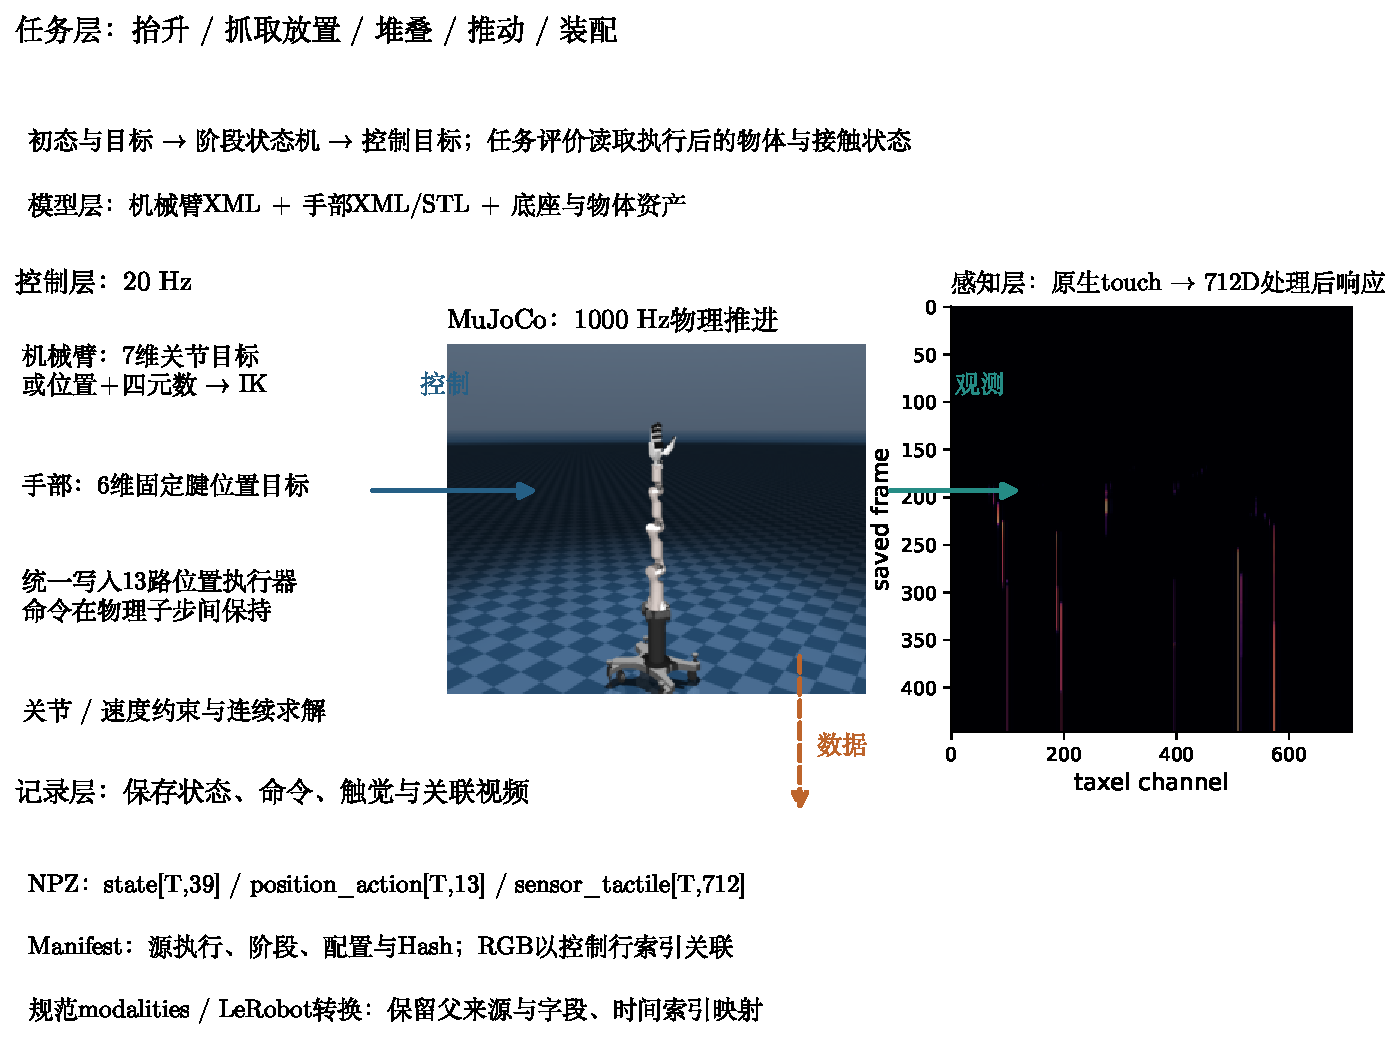
\includegraphics[width=0.97\textwidth]{figures/annotation_R2/platform_actual_architecture.pdf}
  \caption{仿真平台模块及控制、观测数据流}
  \label{fig:ch02_architecture}
\end{figure}

\begin{table}[htbp]
  \centering\small
  \caption{仿真平台主要模块与功能}
  \label{tab:ch02_modules}
  \begin{tabular}{p{0.15\textwidth}p{0.32\textwidth}p{0.39\textwidth}}
    \hline
    模块 & 主要组成 & 接口职责\\
    \hline
    模型层 & 模型描述、资产与组合构建器 & 确定关节、执行器、几何及安装关系\\
    控制层 & 机械臂与手部位置控制器 & 将动作转换为执行器控制量\\
    感知层 & 曲面阵列与信号处理器 & 绑定传感器地址并输出有序观测\\
    任务层 & 场景、任务状态与评价器 & 设置任务条件并评价执行状态\\
    记录层 & 在线记录及合同检查 & 保存关联记录并检查数组合法性\\
    \hline
  \end{tabular}
\end{table}

一次控制周期中，环境先将动作送入控制器，再推进若干物理子步，随后读取观测并进行任务评价。记录模块位于执行链路的接口处，不参与接触力求解。这样的顺序有助于区分控制目标、物理状态和观测结果，避免把目标动作直接当成已经完成的运动。

平台设置Lift、PickPlace、Stack、Push和NutAssembly五类任务接口，分别面向抬升、搬移放置、堆叠、推动和装配过程。任务工厂负责选择任务对象，并由任务实例补充相应场景。接口注册说明软件具有对应入口，但不能代替具体条件下的执行验证。本章仅以已有代表性记录核查观测输出，抓取生成与任务性能分析在第三章展开，数据组织及质量控制在第四章讨论。

\section{RM75B机械臂与途见科技自研灵巧手模型}
\label{sec:robot_model}

机器人组合模型选用与实验室设备型号对应的RM75B机械臂及途见科技自研欠驱动灵巧手，并通过底座和末端安装变换完成组合。XML规定关节、驱动和刚体连接，STL保存连杆与皮肤形状，URDF保留机构描述参考；当前构建器实际加载XML及其网格资产，统一模型接口。本文在该资产配置上研究控制与感知布局，几何尺寸误差、动力学参数和触觉响应的实机标定作为后续验证内容。机械臂采用MuJoCo模型描述格式（MuJoCo Modeling Format，MJCF），以XML文件组织刚体、关节、执行器和传感器。该模型定义七个串联转动关节，依次命名为joint1至joint7，其位置目标分别由pos\_joint1至pos\_joint7执行器接收。各关节的轴、范围与连杆变换由XML给定，控制器据执行器关联关系定位实际关节地址，而不是假定它们在状态数组中始终连续排列。七自由度结构为末端位姿调节提供冗余，但冗余自由度能否用于避碰或姿态优化，还取决于实际控制目标和求解约束，不能仅由关节数量推断。

机械臂各级连杆通过局部位置和四元数描述相对变换，末端定义right\_hand安装体和right\_hand\_site。安装体用于附着手部模型，末端site用于位姿读取及逆运动学计算，两者职责不同。组合构建器将手部安装到指定body，并施加机械臂描述中给定的附加旋转，其XYZ欧拉角为$(-90^\circ,-90^\circ,0^\circ)$。该旋转通过四元数参与坐标组合，必须与父body原有变换共同使用。因此，附加安装角不能直接解释为灵巧手在世界坐标系中的姿态。对于定义在几何局部坐标系中的点，其所属刚体坐标由旋转和平移共同确定；同样的变换规则也用于后续触觉采样点安装。

\begin{figure}[htbp]
  \centering
  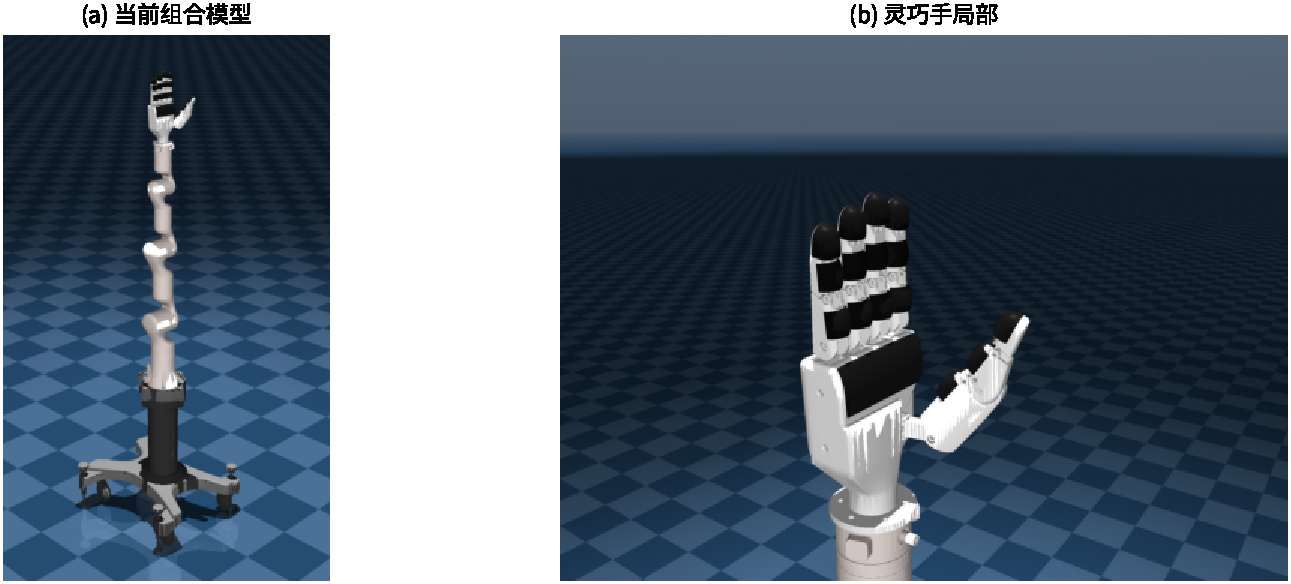
\includegraphics[width=0.96\textwidth]{figures/revision_20261127/robot_model.pdf}
  \caption{当前XML/STL模型的MuJoCo静态渲染：机械臂、底座与灵巧手组合及手部局部（关节零位）}
  \label{fig:ch02_robot_model}
\end{figure}

当前途见科技灵巧手模型含十二个转动关节，由六个固定腱和六个位置执行器驱动。其中四个手指分别具有两个转动关节，每指两个关节共同受一个屈曲腱驱动；拇指包含对掌关节及三个屈曲关节，对掌与屈曲分别对应一个驱动通道。手指上的三个触觉Patch不意味着三个独立关节：部分皮肤几何附着于同一指节刚体。模型需要分别记录机构自由度、执行器数量和感知区域数量，三者不存在一一对应关系。

固定腱通过关节坐标的线性组合定义传动长度，其关系写为
\begin{equation}
  l_t=\sum_{j\in\mathcal J_t}c_{tj}q_j,
  \label{eq:ch02_tendon}
\end{equation}
其中，$q_j$为第$j$个关节角，$\mathcal J_t$为第$t$个固定腱关联的关节集合，$c_{tj}$为XML中给定的传动系数。四指屈曲腱对两个关节均使用0.003的系数；拇指对掌系数为0.0085，屈曲腱的三个系数依次为0.0035、0.004和0.004。在模型长度约定下，控制目标对应腱坐标，不是各手指关节的独立角度目标。这些系数描述当前仿真传动，不作为实机推杆尺寸的测量结果。

\begin{figure}[htbp]
  \centering
  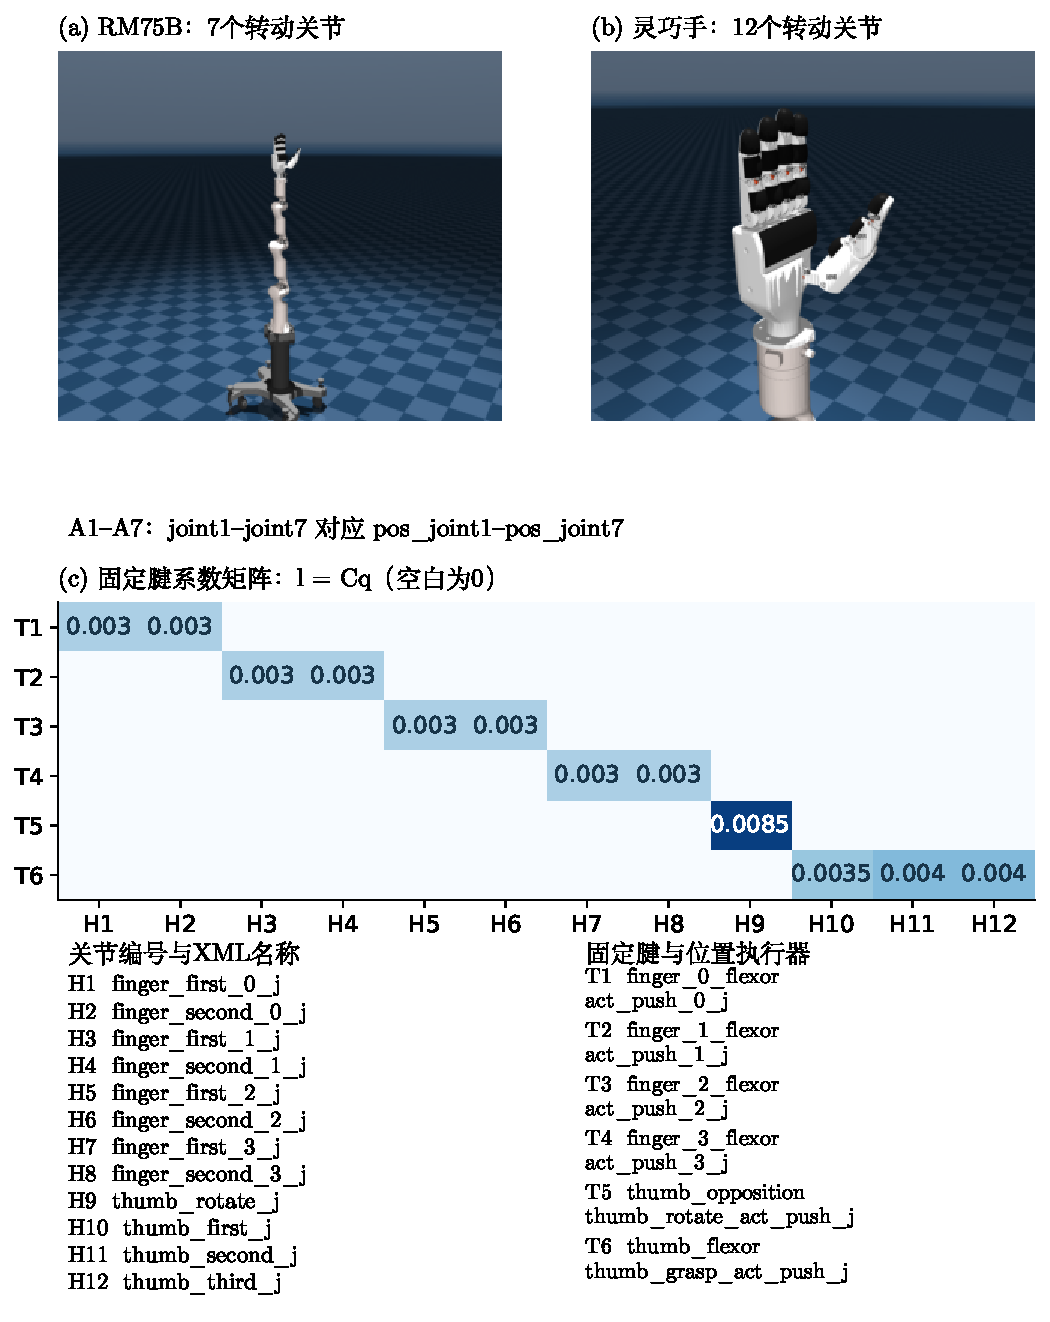
\includegraphics[width=0.97\textwidth]{figures/annotation_R2/joint_tendon_geometry.pdf}
  \caption{当前MuJoCo关节几何与XML固定腱系数、执行器对应关系}
  \label{fig:ch02_drive}
\end{figure}

\begin{table}[htbp]
  \centering\small
  \caption{机械臂及灵巧手执行器配置}
  \label{tab:ch02_actuators}
  \begin{tabular}{p{0.26\textwidth}p{0.23\textwidth}p{0.24\textwidth}p{0.13\textwidth}}
    \hline
    执行器或通道 & 控制坐标范围 & 比例增益$k_p$ & 输出限幅\\
    \hline
    pos\_joint1 & $[-3.1,3.1]$ rad & 5000 & $\pm60$ N$\cdot$m\\
    pos\_joint2 & $[-2.268,2.268]$ rad & 5000 & $\pm60$ N$\cdot$m\\
    pos\_joint3 & $[-3.1,3.1]$ rad & 3000 & $\pm30$ N$\cdot$m\\
    pos\_joint4 & $[-2.355,2.355]$ rad & 3000 & $\pm30$ N$\cdot$m\\
    pos\_joint5 & $[-3.1,3.1]$ rad & 2000 & $\pm10$ N$\cdot$m\\
    pos\_joint6 & $[-2.233,2.233]$ rad & 2000 & $\pm10$ N$\cdot$m\\
    pos\_joint7 & $[-6.28,6.28]$ rad & 1000 & $\pm10$ N$\cdot$m\\
    四指屈曲，各1通道 & $[0,0.01]$ m & 10000 & $\pm20$ N\\
    拇指对掌 & $[-0.0069,0.004]$ m & 4000 & $\pm20$ N\\
    拇指屈曲 & $[0,0.01]$ m & 4000 & $\pm20$ N\\
    \hline
  \end{tabular}
\end{table}

手部关节还配置被动弹簧及阻尼。驱动腱提供整体屈曲作用，而不同关节在接触物体后受到不同约束，未受阻关节仍可改变姿态，由此表达模型中的欠驱动适应行为。该机制并不意味着接触后每个关节都获得唯一稳定解，其运动还受弹簧、摩擦及求解参数影响。表\ref{tab:ch02_actuators}采用模型的SI单位约定：机械臂$k_p$单位为N$\cdot$m/rad，腱执行器$k_p$单位为N/m；腱力与关节力矩不能直接比较。这些是仿真参数，不是实物标定值。

手部采用刚体关节与固定腱传动描述欠驱动耦合，执行器通过腱长坐标同时作用于关联关节。模型的机构、安装变换和皮肤几何分别保存在XML、URDF与STL资产中。图\ref{fig:ch02_robot_model}展示安装后的组合模型与手部局部，图\ref{fig:ch02_drive}给出执行器、固定腱和关节之间的传动关系。

\section{灵巧手接触建模与控制方法}
\label{sec:contact_control}

本文实现组合位置控制器，将机械臂目标解释与手部腱驱动控制连接到MuJoCo执行器。设计中将目标求解放在控制周期内，将位置伺服与接触求解交由物理引擎执行：关节模式直接接收位置目标，末端模式先求解逆运动学，两者最终均输出七维机械臂关节目标；手部另接收六维腱位置目标。由此，同一套执行器接口可以服务于关节轨迹和末端轨迹，手部控制也保留其欠驱动传动关系。MuJoCo负责约束下的状态推进\cite{todorov2012mujoco,mujoco2026computation}，组合构建器统一采用Newton求解器、100次迭代上限、椭圆摩擦锥与0.001~s物理步长。

手部皮肤以mesh几何参与碰撞。padgeom默认接触维数为4，包括法向约束、两个切向滑动摩擦方向和绕接触法向的扭转摩擦方向，用于描述指面接触对滑移与转动的阻碍\cite{mujoco2026xml}。滑动、扭转和滚动摩擦配置值分别为1.3、0.02和0.0002；滚动摩擦方向在六维接触中使用，实际启用维数由接触配对规则确定。接触参考参数$(0.01,1)$采用正值格式，分别表示0.01~s时间常数和阻尼比1，用于设置约束恢复的柔顺性与阻尼。部分手指与拇指、手掌与手指之间另有显式pair，物体与桌面也有各自参数。碰撞求解采用皮肤mesh，感知布局则从同一资产派生采样点，两者分别承担接触计算与读出区域布置。

机械臂position模式将七维动作解释为关节位置目标，经合法范围约束后写入执行器控制数组。IK模式则接受末端位置与四元数组成的七维目标，在临时状态上迭代求解关节配置。设机械臂关节向量为$\boldsymbol q\in\mathbb R^7$，位置误差为$\boldsymbol e_p\in\mathbb R^3$，四元数误差转换得到的旋转向量为$\boldsymbol e_r\in\mathbb R^3$。代码分别调用末端site的位置与旋转Jacobian，按权重组成$\boldsymbol J_w$及$\boldsymbol e_w$。这里的旋转误差不是欧拉角逐分量相减，位置与旋转权重则用于调整两类误差在数值求解中的相对作用。

对加权Jacobian作奇异值分解后，控制器使用阻尼伪逆计算主任务修正，并在启用时叠加姿态项：
\begin{equation}
 \begin{aligned}
  \boldsymbol J_w&=\boldsymbol U\boldsymbol\Sigma\boldsymbol V^{\mathsf T},\qquad
  \boldsymbol J_{\lambda}^{+}=\boldsymbol V\,
  \operatorname{diag}\!\left(\frac{\sigma_i}{\sigma_i^2+\lambda^2}\right)
  \boldsymbol U^{\mathsf T},\\
  \Delta\boldsymbol q&=\boldsymbol J_{\lambda}^{+}\boldsymbol e_w+
  \left(\boldsymbol I-\boldsymbol J_{\lambda}^{+}\boldsymbol J_w\right)
  k_n(\boldsymbol q_0-\boldsymbol q).
 \end{aligned}
 \label{eq:ch02_ik}
\end{equation}
其中，$\sigma_i$为奇异值，$\lambda$为阻尼系数，$k_n$为姿态调节增益。默认开启零空间项且$k_n=0.1$；未显式指定时，$\boldsymbol q_0$取各关节执行器控制上下限的中点，当前机械臂对应七维零向量。阻尼能够限制小奇异值对应的更新放大，代码还依据奇异值和条件数调整阻尼。式\ref{eq:ch02_ik}中的第二项仅在零空间选项开启时使用；由于采用阻尼伪逆，其投影不应解释为对主任务完全无影响的严格正交零空间。另一个参数posture\_weight控制在误差与Jacobian中追加加权姿态残差，其默认值0仅关闭该附加残差，不关闭上述零空间项。式\ref{eq:ch02_ik}对应默认设置下SVD成功的路径；SVD失败时退回阻尼最小二乘求解，该分支不叠加零空间项。迭代达到位姿容差后可提前退出，所得目标还需进行关节限幅及速度平滑。指定profile采用position模式，不调用该IK求解路径。

\begin{figure}[htbp]
  \centering
  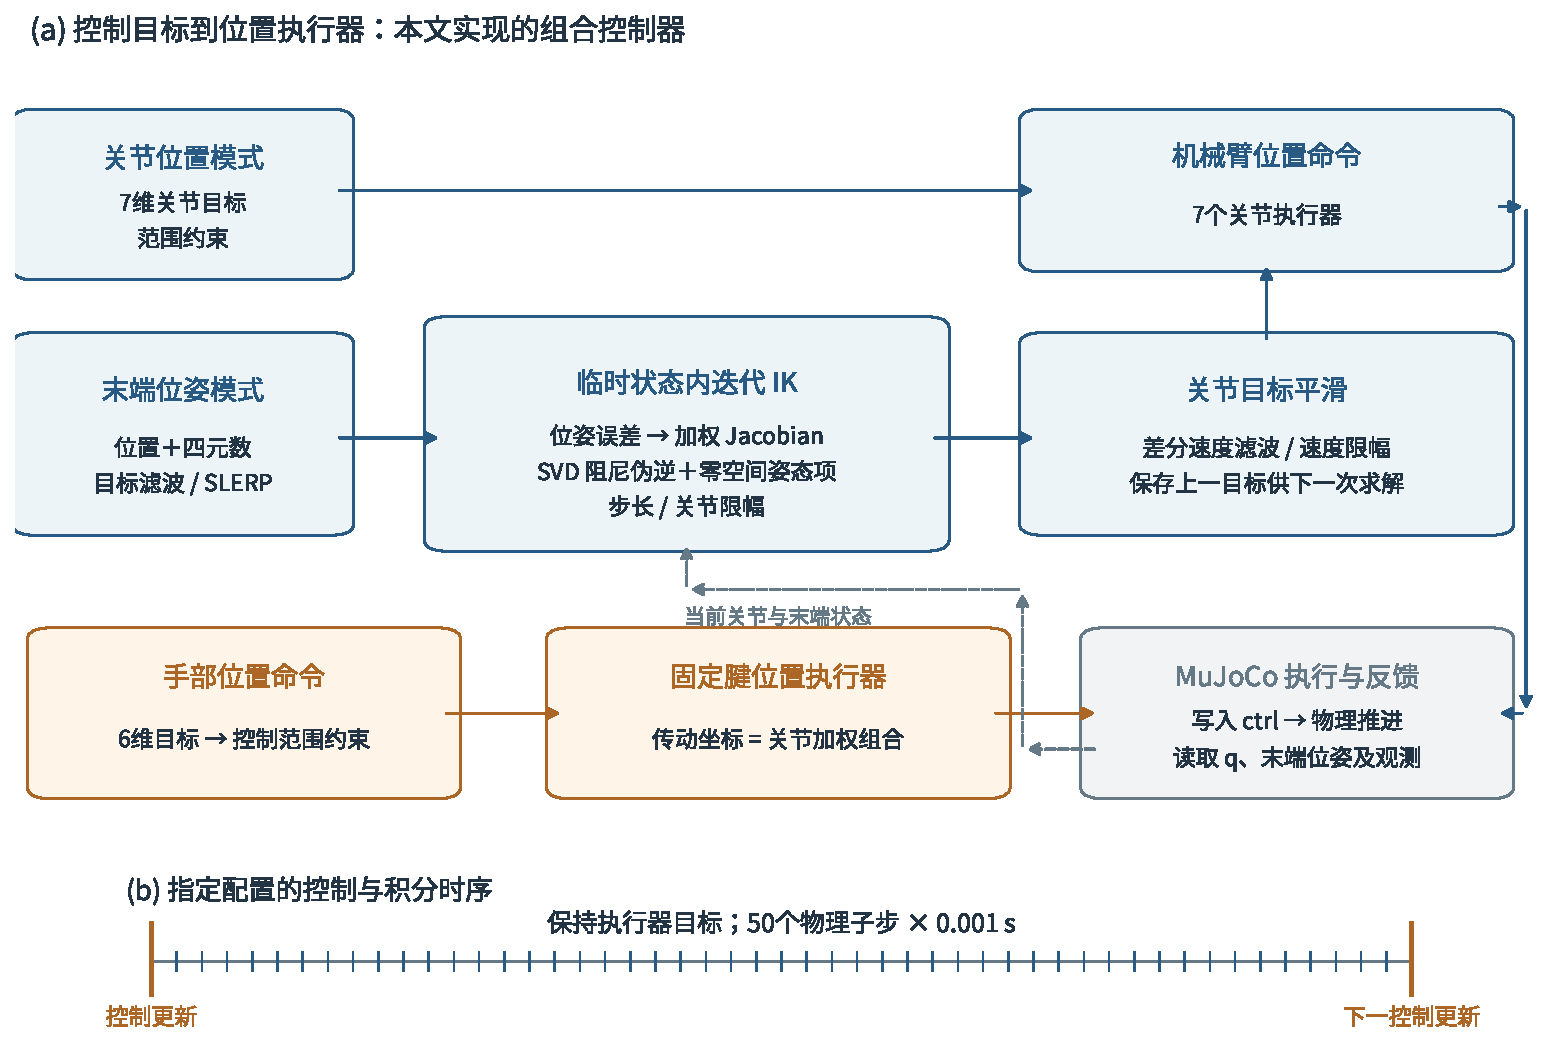
\includegraphics[width=0.97\textwidth]{figures/annotation_batch2/control_implementation.pdf}
  \caption{组合控制器的目标求解、执行器接口及多速率执行}
  \label{fig:ch02_control}
\end{figure}

\begin{table}[htbp]
  \centering\small
  \caption{主要控制与物理参数及其适用范围}
  \label{tab:ch02_control_parameters}
  \begin{tabular}{p{0.28\textwidth}p{0.23\textwidth}p{0.35\textwidth}}
    \hline
    参数 & 取值 & 配置层级\\
    \hline
    物理步长、求解器 & 0.001~s，Newton & 组合构建器覆盖值\\
    求解迭代上限、摩擦锥 & 100，椭圆锥 & 组合构建器覆盖值\\
    控制周期 & 0.05~s & 指定机器人profile\\
    IK迭代上限、初始阻尼 & 80，$10^{-3}$ & 控制器构造默认值\\
    位置、旋转误差权重 & 1，0.35 & 控制器构造默认值\\
    位置、旋转误差容差 & $10^{-4}$~m，$10^{-3}$~rad & 控制器构造默认值\\
    单次关节修正上限 & 0.15~rad & 控制器构造默认值\\
    目标关节速度上限 & 2~rad/s & 控制器构造默认值\\
    零空间调节增益 & 0.1 & 默认开启，可由调用方配置\\
    附加姿态残差权重 & 0 & 不影响零空间项的默认开关\\
    \hline
  \end{tabular}
\end{table}

图\ref{fig:ch02_control}给出两种机械臂模式及手部控制的汇合关系。IK求解在临时状态中迭代，以上一关节目标作连续求解初值，并在输出前进行速度滤波和限幅；实际仿真状态在随后的物理推进中更新。手部控制器接收六个位置通道，并根据执行器的传动类型读取坐标。固定腱执行器的位置由其关联关节的加权组合确定，控制器据此读取腱传动坐标，并与目标腱长比较。底层由MJCF位置执行器及其阻尼设置完成伺服，而不是在控制代码中另设一个通用力矩PD控制器\cite{mujoco2026xml}。表\ref{tab:ch02_control_parameters}列出控制器的默认参数，具体任务可在构造时覆盖。

指定profile的控制周期为0.05~s，环境按其与物理步长之比确定每周期50个子步，对应20~Hz控制和1000~Hz物理积分。图\ref{fig:ch02_control}中，动作只在控制周期开始时更新，执行器目标在子步内保持，环境完成物理推进后读取观测。物理积分频率决定状态推进间隔，观测采样频率决定保存时刻。接触可能在子步内出现或消失，因此20~Hz观测并不包含所有物理子步上的瞬态变化，这也是解释触觉时序时需要保留的采样边界。

\section{复杂曲面触觉阵列建模}
\label{sec:curved_tactile_array}

灵巧手指节和指尖具有不同曲率，直接在固定平面上均匀放置感知区域容易造成区域偏离表面、朝向不一致或局部重复覆盖。平台按实验室灵巧手的指节、指尖和手掌感知区域组织阵列，由相应皮肤STL派生采样点，再将局部位置与朝向安装到所属指节刚体。该建模过程使仿真感知区域随机构运动，并保留区域与通道的对应。阵列按手指与手掌的感知区域组织，使采样位置随各指节刚体运动，并保持固定的通道顺序。与以图像合成为主要输出的视觉触觉模拟器\cite{wang2022tacto,si2022taxim}不同，本平台在曲面附近布置原生touch感知区域，输出有序标量阵列。

每个手指设置近端、另一指节区域和指尖三个Patch，前两者为$4\times8$，指尖为$7\times8$；手掌设置$7\times16$阵列。五指共600个单元，手掌112个单元，总计16个Patch、712个感知单元。图\ref{fig:ch02_patch_order}按仿真索引展示布局组织，具体区间见表\ref{tab:ch02_patch_layout}。各区域的采样点分别由所属STL计算，以适应指节、指尖与手掌的曲率差异。

\begin{figure}[htbp]
\centering
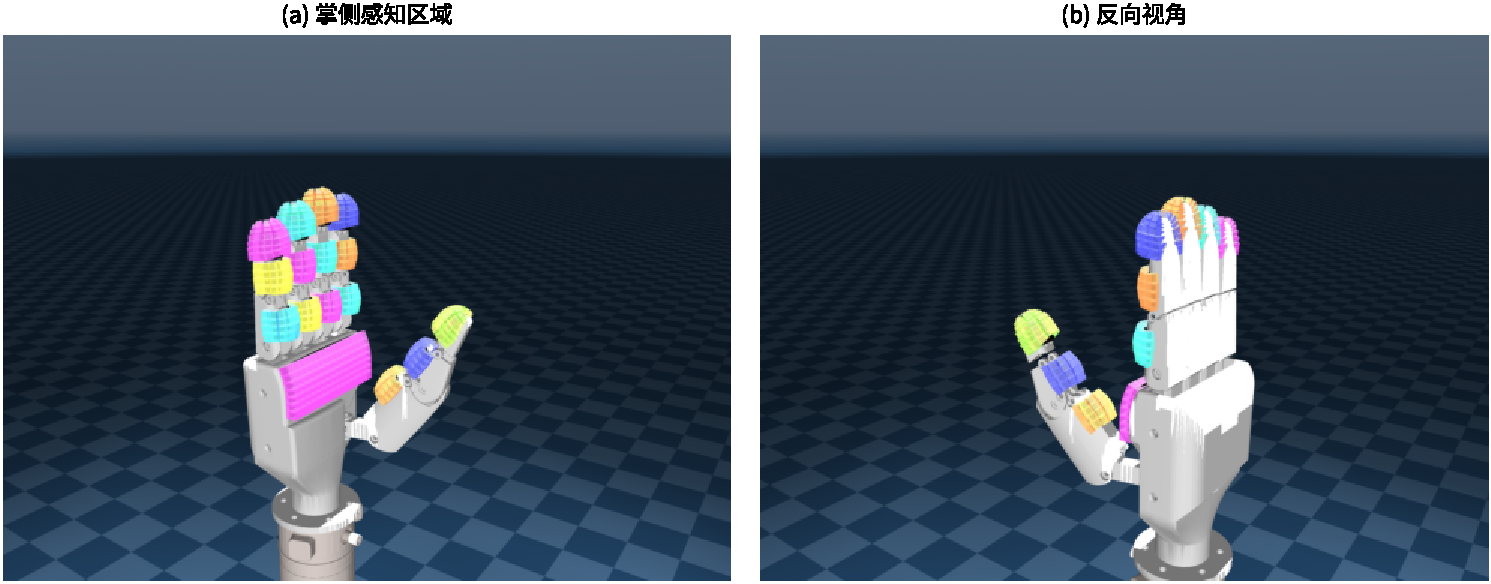
\includegraphics[width=0.97\textwidth]{figures/revision_20261127/tactile_layout.pdf}
\caption{当前MuJoCo模型中的16个Patch与712个box感知区域（颜色区分局部阵列）}
\label{fig:ch02_patch_order}
\end{figure}

segment策略面向指节皮肤。实现先对三角网格进行加密采样，通过主成分分析建立局部轴向与截面方向，再结合三角面朝向及径向分布筛选外表面。主成分方向来自几何点云的主要变化方向，并不自动具有固定的实物解剖含义。截面拟合和有效角度范围用于构造连续外壳样本，随后将样本组织成规则参数网格。与直接按原网格顶点布点相比，该过程能够减少三角网格局部密度差异对阵列索引分布的直接影响，但不保证最终点间距处处相等。

对规则外壳样本，程序拟合张量积Bezier曲面。设参数$u,v\in[0,1]$，控制点为$\boldsymbol C_{ij}\in\mathbb R^3$，曲面及其拟合关系为
\begin{equation}
 \begin{aligned}
  \boldsymbol S(u,v)&=\sum_{i=0}^{d_u}\sum_{j=0}^{d_v}
    B_i^{d_u}(u)B_j^{d_v}(v)\boldsymbol C_{ij},\\
  (\boldsymbol A^{\mathsf T}\boldsymbol W\boldsymbol A+\rho\boldsymbol I)\boldsymbol C
    &=\boldsymbol A^{\mathsf T}\boldsymbol W\boldsymbol P.
 \end{aligned}
 \label{eq:ch02_bezier}
\end{equation}
其中，$B_i^{d_u}$和$B_j^{d_v}$为Bernstein基函数，$\boldsymbol A$为采样参数对应的设计矩阵，$\boldsymbol P$存储三维样本，$\boldsymbol W$为样本权重。正则强度$\rho$由配置系数与加权设计矩阵的平均对角尺度共同确定，不能直接等同于配置中的无量纲系数。曲面坐标沿用网格的长度单位，参数坐标本身无量纲。最终Taxel位于参数单元中心，避免将相邻单元同时放到同一边界上。

指尖策略的配置名称为fingertip-ellipsoid，但当前函数体并非在理想椭球上直接布点。它先识别指尖的swept-shell外壳，分析轴向切片及外侧包络，再对规则样本拟合Bezier曲面。指尖拟合使用更高的轴向次数及边界权重，以表达末端弯曲和封闭区域；最终轴向参数在$[0.06,1]$范围分格后取中心，而不是把最后一行放到参数极点。这样能够避免指尖极点附近多列采样重合。



手掌采用mesh-uv策略。程序对网格进行PCA投影，在局部二维参数域内设置规则采样位置，再通过投影三角形的重心坐标插值恢复三维点。当多个表面投影重叠时，需要选择对应外表面；当采样位置落在投影缺口或边界之外时，使用实现中的最近三角形回退。该方法保留了采样点与网格的关系，但二维规则网格不等于曲面等面积划分，投影折叠和回退区域也可能产生不同的局部间距。表\ref{tab:ch02_layout_parameters}列出三类布局的关键差异，不能仅根据策略名称推断其几何性质。

图\ref{fig:ch02_fingertip}对照展示三类策略的代表形状：两个指节区域采用segment，指尖采用swept-shell外壳识别与Bezier拟合，手掌采用mesh-uv。各子图均使用对应STL和实际采样函数生成；灰色表示原始网格，橙色表示采样中心，连线仅表示阵列行列邻接。坐标沿用各网格局部坐标系，轴单位由米换算为毫米，各子图独立取尺度，不代表统一安装姿态或真实电极标定。
\begin{figure}[htbp]
  \centering
  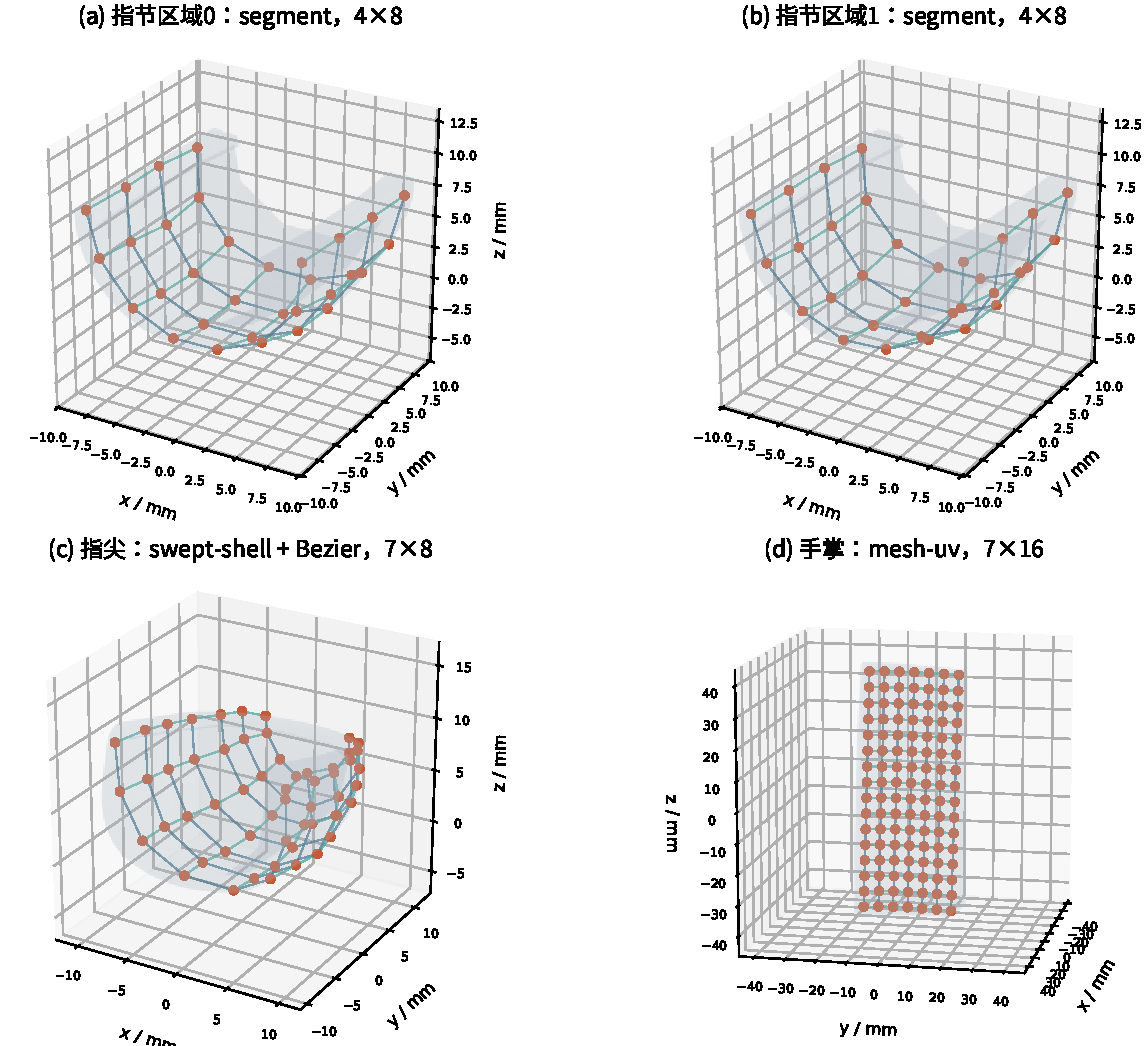
\includegraphics[width=0.97\textwidth]{figures/revision_20261127/surface_layout_strategies.pdf}
  \caption{三类曲面采样策略在指节、指尖和手掌代表网格上的布局（网格局部坐标）}
  \label{fig:ch02_fingertip}
\end{figure}


\begin{table}[htbp]
  \centering\small
  \caption{不同曲面布局方法的关键实现参数}
  \label{tab:ch02_layout_parameters}
  \begin{tabular}{p{0.18\textwidth}p{0.29\textwidth}p{0.39\textwidth}}
    \hline
    配置策略 & 外壳或参数域构造 & 拟合及最终采样\\
    \hline
    segment & PCA轴向、截面及外壳筛选 & Bezier次数$(5,7)$；正则系数$5\times10^{-5}$；参数单元中心\\
    指尖策略 & swept-shell外包络 & Bezier次数$(6,7)$；正则系数$8\times10^{-6}$；边界权重10\\
    mesh-uv & PCA二维投影 & 三角形重心插值；外侧选择与缺口回退\\
    \hline
  \end{tabular}
\end{table}

三类策略的区别来自表面几何：指节适合沿主要轴向组织截面，指尖需要处理封闭弯曲外壳与极点，手掌则通过投影三角形保留不规则网格。图\ref{fig:ch02_sampling_steps}给出实际采样函数的中间输出。指节和指尖先从STL识别密集外壳样本，再按各自Bezier配置拟合并取参数单元中心；手掌在PCA参数域设置格点，通过三角形定位与重心插值恢复三维位置。图中从原始几何到密集样本、再到最终阵列的变化，展示了规则索引如何依附不同曲面，而非将三种形状套用同一平面网格。

\begin{figure}[p]
 \centering
 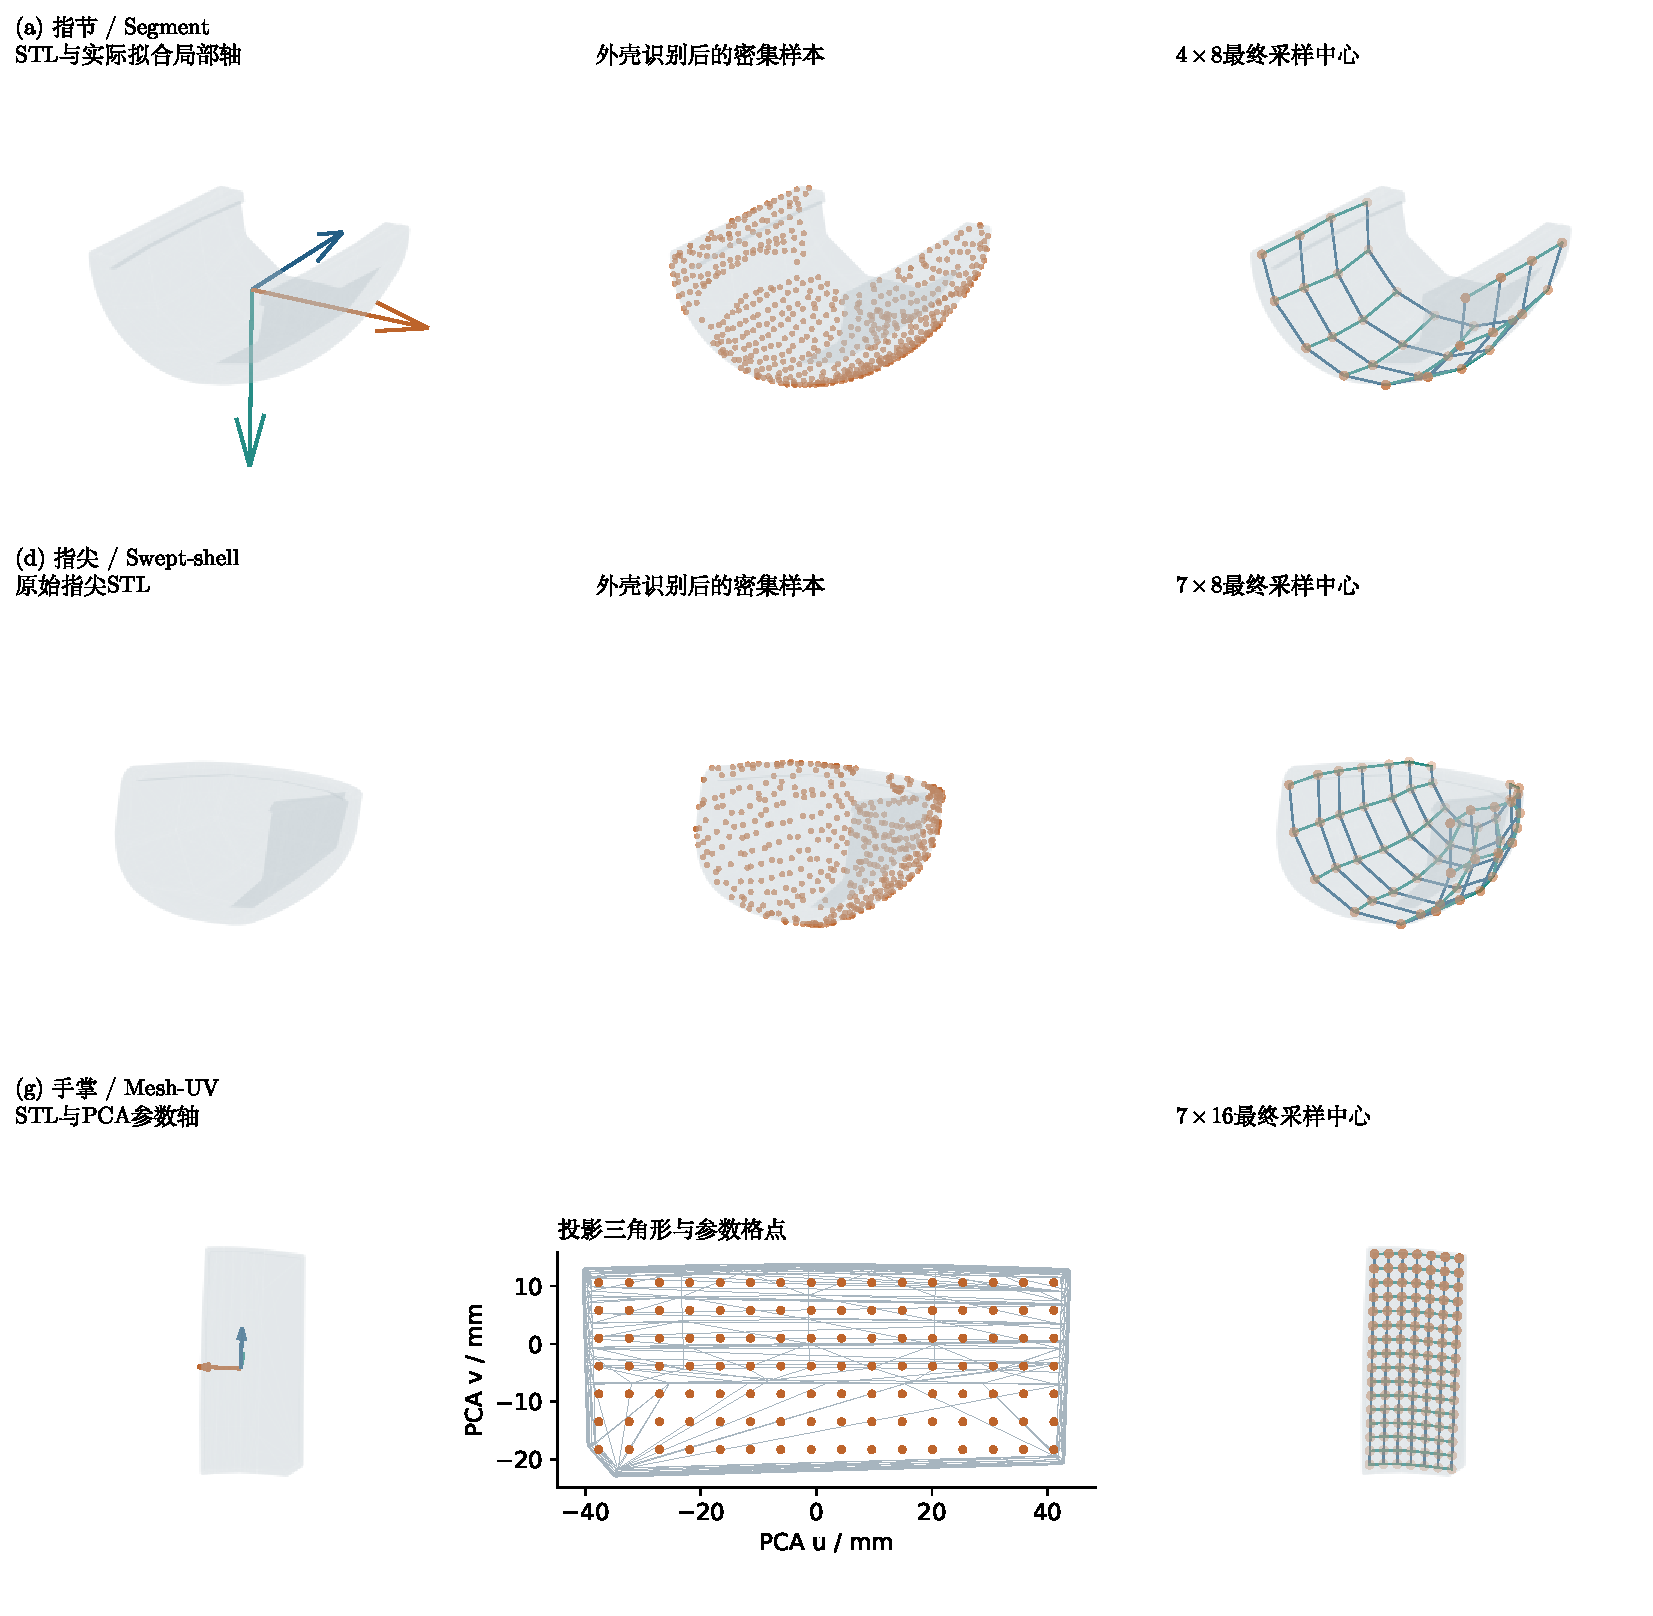
\includegraphics[width=0.98\textwidth,height=0.80\textheight,keepaspectratio]{figures/annotation_R2/sampling_processes.pdf}
 \caption{三类曲面采样的实际中间输出：STL与局部轴、外壳或参数域、最终采样中心}
 \label{fig:ch02_sampling_steps}
\end{figure}

对图中三个代表区域，最终采样点最近邻距离的最小值与中位数分别为：指节3.609/3.910~mm，指尖1.504/3.034~mm，手掌4.820/4.866~mm。距离按各点到其余采样点的最小欧氏距离计算，描述本次几何布局中的间距变化；曲率、感知区尺寸及接触覆盖还需结合各自模型分析。

网格采样点还需安装到正确的刚体上。程序先应用skin geom的局部旋转和平移，再根据行列相邻点差分构造切线。列方向归一化为$\boldsymbol e_x$，行方向经Gram--Schmidt正交化得到$\boldsymbol e_y$，法向由两者叉乘确定，局部方向矩阵为$[\boldsymbol e_x,\boldsymbol e_y,\boldsymbol n]$。随后依据点相对body或Patch参考位置进行外向修正。该步骤是保持感知区朝向一致的几何启发式，不能称为已经认证的实物表面法线。图\ref{fig:ch02_frame}展示局部切线与叉乘法向，特意区分外向修正前的坐标构造。

\begin{figure}[htbp]
  \centering
  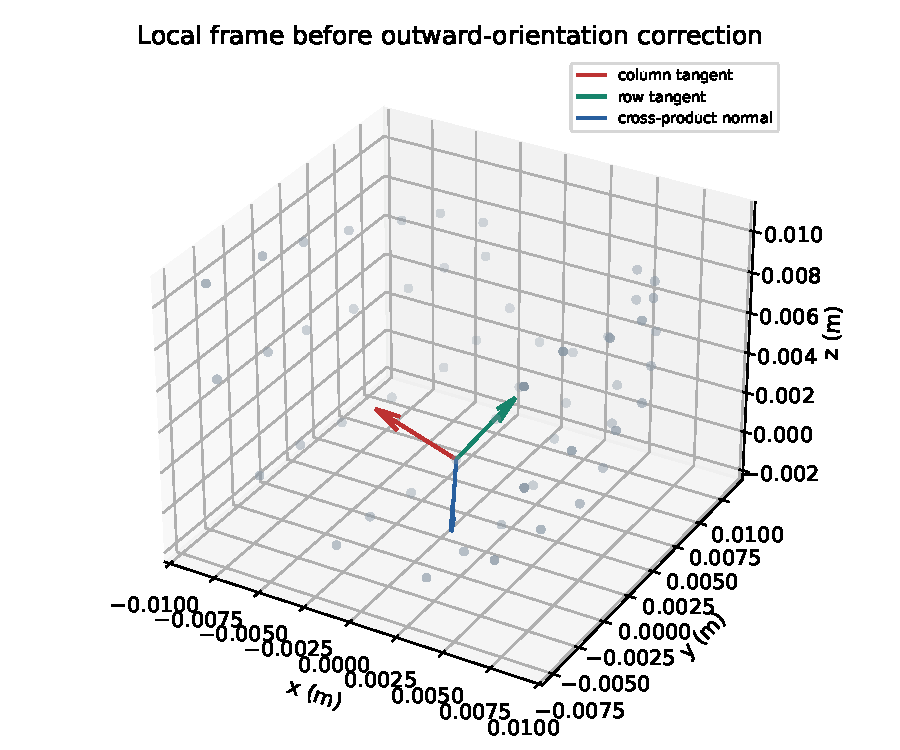
\includegraphics[width=0.66\textwidth]{figures/ch02/taxel_local_frame.pdf}
  \caption{由相邻采样点构造的局部切线和法向（外向修正前）}
  \label{fig:ch02_frame}
\end{figure}

每个采样点对应一个定向box site。其切向半宽分别依据列、行相邻距离设置：
\begin{equation}
 h_x=\max\!\left(h_{\min},\frac{\gamma d_c}{2}\right),\qquad
 h_y=\max\!\left(h_{\min},\frac{\gamma d_r}{2}\right).
 \label{eq:ch02_site_size}
\end{equation}
其中，$d_c,d_r$为对应方向可用相邻距离的最小值，$\gamma$为overlap系数，$h_{\min}$为最小半宽；法向半厚度$h_z$单独配置。指定profile取$\gamma=1.25$、$h_{\min}=0.0005$~m、$h_z=0.004$~m，而传感器类默认厚度和overlap分别为0.0015~m和1.0。二者必须按具体配置区分。box site用于指定有体积的感知区域，碰撞仍由皮肤几何参与计算；相邻感知区域允许重叠，以减少采样间隙。

\begin{table}[htbp]
  \centering\small
  \caption{16个Patch的阵列规格与712维索引区间}
  \label{tab:ch02_patch_layout}
  \begin{tabular}{llll}
    \hline
    Patch名称 & 行$\times$列 & 零基右开区间 & 布局类别\\
    \hline
    skin\_0\_0\_p & $4\times8$ & $[0,32)$ & segment\\
    skin\_0\_1\_p & $4\times8$ & $[32,64)$ & segment\\
    skin\_0\_2\_p & $7\times8$ & $[64,120)$ & 指尖策略\\
    skin\_1\_0\_p & $4\times8$ & $[120,152)$ & segment\\
    skin\_1\_1\_p & $4\times8$ & $[152,184)$ & segment\\
    skin\_1\_2\_p & $7\times8$ & $[184,240)$ & 指尖策略\\
    skin\_2\_0\_p & $4\times8$ & $[240,272)$ & segment\\
    skin\_2\_1\_p & $4\times8$ & $[272,304)$ & segment\\
    skin\_2\_2\_p & $7\times8$ & $[304,360)$ & 指尖策略\\
    skin\_3\_0\_p & $4\times8$ & $[360,392)$ & segment\\
    skin\_3\_1\_p & $4\times8$ & $[392,424)$ & segment\\
    skin\_3\_2\_p & $7\times8$ & $[424,480)$ & 指尖策略\\
    skin\_4\_0\_p & $4\times8$ & $[480,512)$ & segment\\
    skin\_4\_1\_p & $4\times8$ & $[512,544)$ & segment\\
    skin\_4\_2\_p & $7\times8$ & $[544,600)$ & 指尖策略\\
    skin\_palm\_p & $7\times16$ & $[600,712)$ & mesh-uv\\
    \hline
  \end{tabular}
\end{table}

阵列索引按手指0至4、每指Patch 0至2、最后手掌的顺序连接，各Patch内部采用行主序。索引顺序同时服务于传感器命名、观测展开与后处理还原，因而必须保持一致。该组织保证了仿真内部从曲面位置到数组通道的可追溯性，但不认证实机电气通道到同名索引的物理对应。后续展示触觉时可将区间恢复为原二维方阵，而不是把712个通道当作一条具有物理邻接关系的长序列。

曲面阵列的构建步骤归纳为算法\ref{alg:curved_tactile_build}。其输出为模型内的感知区域及传感器索引，不是独立碰撞单元或经标定的真实电极。
\begin{algorithm}[H]
\small
\caption{曲面触觉阵列构建}\label{alg:curved_tactile_build}
\KwIn{皮肤网格、所属刚体变换、16个Patch布局与尺寸配置}
\KwOut{712个box site、touch传感器及有序地址映射}
\ForEach{按既定顺序遍历的Patch $p$}{
读取对应STL及行列数，按配置布局策略计算曲面采样点\;
将网格坐标转换至所属刚体局部坐标，核对点数\;
\ForEach{按行主序遍历的采样点}{
由相邻差分构造切线并正交化，确定朝外局部坐标系\;
由邻域间距、overlap及最小半宽计算site尺寸\;
向所属刚体添加box site，并关联原生touch传感器\;
}
}
编译模型，绑定传感器地址并登记Patch索引区间\;
\end{algorithm}

\section{712维触觉观测及处理流程}
\label{sec:tactile_processing}

曲面布局确定感知区域的位置，触觉读出则决定每个区域记录什么量。构建器在组合手部之前调用传感器的augment\_spec接口，为每个采样点添加box site和一个MuJoCo原生mjSENS\_TOUCH传感器。模型完成构建后，bind依据传感器名称查找编号，检查输出维数为1，并保存sensor\_adr所指示的数据地址。地址与传感器编号不是同一概念，其他类型传感器可能占据不同长度的sensordata区间。read\_raw按已绑定地址读取712个值并转换为float32副本，避免后续物理更新改变已经返回的数组。

原生touch在相应body和site感知条件下累加接触法向力，输出非负标量\cite{mujoco2026xml}。在模型采用SI单位的约定下，它可解释为模拟法向力读数，但没有除以真实电极面积，也不包含完整切向力向量。一个接触可能被重叠感知区重复覆盖，因此全部Taxel读数求和不必等于机器人受到的总外力。该读出也不等同于视觉触觉图像或材料内部连续压力场\cite{si2022taxim,sferrazza2022simtoreal}。当前模型将上述box感知区域与原生touch逐一绑定，再按固定索引读取712维响应。

\begin{figure}[htbp]
  \centering
  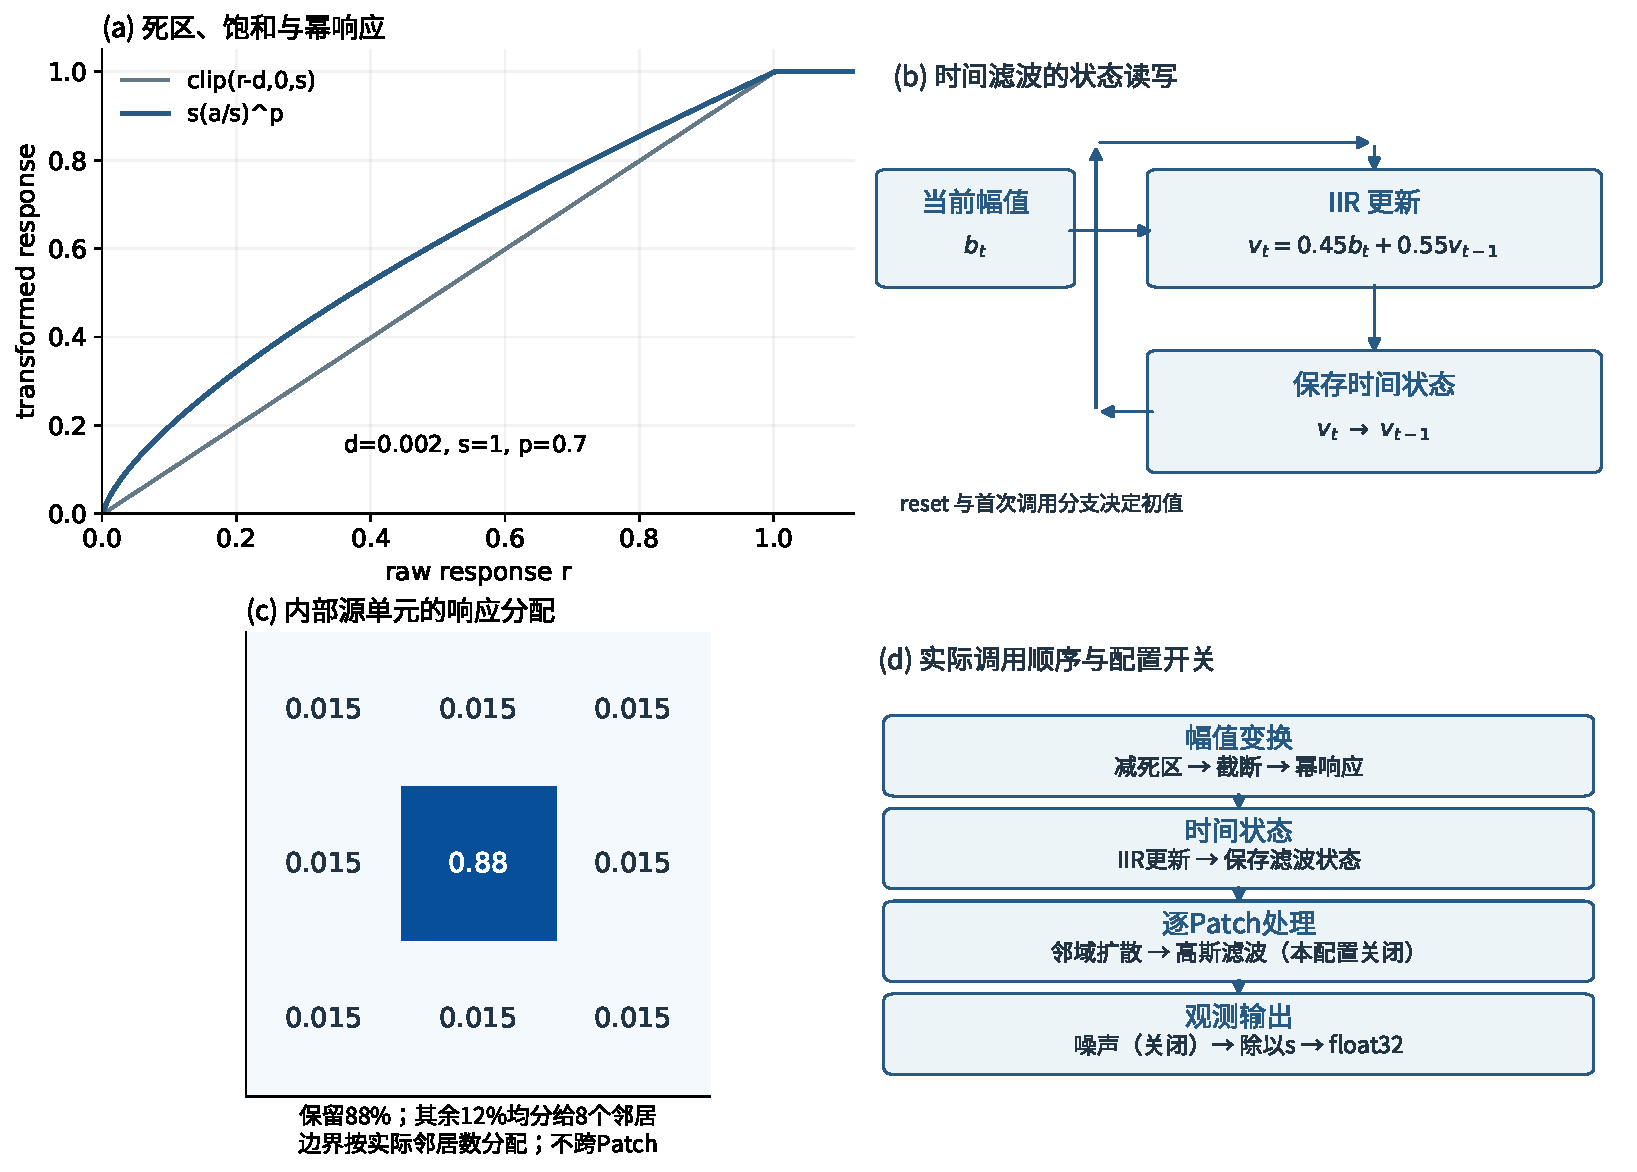
\includegraphics[width=0.97\textwidth]{figures/annotation_batch2/tactile_processing_operators.pdf}
  \caption{触觉幅值、时间与邻域处理算子及调用顺序（指定参数的公式示意）}
  \label{fig:ch02_processing}
\end{figure}

原始数组进入TactileSignalProcessor后，按图\ref{fig:ch02_processing}处理。设原始读数为$r_{t,j}$，死区为$d$，饱和尺度为$s$，幂指数为$p$，低通系数为$\alpha$，主要幅值处理写为
\begin{equation}
 \begin{aligned}
 a_{t,j}&=\operatorname{clip}(r_{t,j}-d,0,s),\qquad
 b_{t,j}=s(a_{t,j}/s)^p,\\
 v_{t,j}&=\alpha b_{t,j}+(1-\alpha)v_{t-1,j},\\
 \boldsymbol y_t&=\operatorname{float32}\!\left(
 \frac{\operatorname{clip}(\mathcal C_c(\boldsymbol v_t),0,s)}{s}\right).
 \end{aligned}
 \label{eq:ch02_processing}
\end{equation}
其中，$t$为连续调用的观测索引，$\mathcal C_c$为下述Patch内邻域扩散算子，$\boldsymbol y_t$为processed向量。末行适用于当前关闭高斯滤波和噪声、开启归一化的profile：先完成邻域扩散及范围限制，再除以饱和尺度$s$，最后转换为float32。滤波初态由处理器reset路径决定，不能假定任何数据片段都以相同方式独立初始化。指定profile使用$d=0.002$、$s=1$、$p=0.7$、$\alpha=0.45$，并开启归一化。死区和饱和设置改变了弱响应及尾部范围，幂变换与时间滤波又改变幅值和相邻观测关系，因此处理后的值不再保留原始模拟力的直接单位含义。

邻域扩散在每个Patch恢复的二维阵列中进行，用于将局部响应分配给邻近单元；图\ref{fig:ch02_processing}(c)显示内部源单元的分配权重。系数$c=0.12$表示每个源单元保留$1-c$的响应，其余部分按可用的8邻域数量平均分配。边界单元的邻居少于内部单元，程序按源单元归一化，不能写成所有接收单元统一除以8。邻域扩散只作用于同一Patch，数组中相邻但属于不同Patch的两个索引不会据此交换响应。当前profile的gaussian\_sigma和noise\_std均为0，高斯滤波与随机噪声属于可选能力，并未在该配置中启用。

\begin{table}[htbp]
  \centering\small
  \caption{触觉观测各阶段的输出与语义}
  \label{tab:ch02_signal_stages}
  \begin{tabular}{p{0.20\textwidth}p{0.27\textwidth}p{0.39\textwidth}}
    \hline
    阶段 & 维度或数据组织 & 处理及适用解释\\
    \hline
    空间布局 & 16个Patch、712个site & 定义感知位置、方向和体积\\
    原生touch & 每site一个非负标量 & 累加满足感知条件的接触法向力\\
    原始读取 & 712维float32副本 & 按sensor\_adr读取，顺序固定\\
    信号处理 & Patch方阵及时间状态 & 死区、截断、幂响应、IIR及邻域扩散\\
    processed输出 & 712维float32 & 指定profile归一化，无量纲响应\\
    \hline
  \end{tabular}
\end{table}

表\ref{tab:ch02_signal_stages}区分了几何采样、原生传感器值和后处理观测。最终向量保持表\ref{tab:ch02_patch_layout}的通道顺序，可还原为局部热图；热图色标只是显示方式，不改变原数组的物理语义。真实采集侧的processed还具有自身驱动和处理条件，不能仅凭同为712维就认为它与仿真观测单位相同。本文在后续跨域研究中保持这一区分，不将无量纲processed数据称为Pa或经过认证的真实压力。

\section{仿真平台功能验证}
\label{sec:platform_validation}

平台验证围绕模型接口、触觉读出和任务记录展开。模型与控制实现提供七个机械臂位置通道、六个手部腱驱动通道以及按传感器名称绑定的触觉地址；组合环境依次完成动作写入、物理推进、观测读取和任务评价。本节进一步分析五条保存的任务记录，检查触觉数组的形状、数值范围、采样时间与激活分布，并用原始视频说明相应操作场景。这样既能检验记录是否符合观测定义，也能观察接触响应在不同操作过程中的变化。

历史观测检查选择五任务开发记录中的五条代表性Episode，分别对应Lift、PickPlace、Stack、Push和NutAssembly。所读取对象为各案例source\_episode目录中的NPZ文件，并结合其manifest与结果记录确认任务来源。核查以完整保存数组为对象，不从中筛选有利时刻；统计字段固定为sensor\_tactile。设单条记录含$T$帧，则触觉合同要求数组为$T\times712$，数据类型为float32，所有元素有限且非负，同时检查是否全零。非零比例在整条数组上计算，用于描述保存响应的稀疏程度，不作为任务成功率或传感器准确率。

\begin{table}[htbp]
  \centering\small
  \caption{五条历史开发Episode的触觉观测核查结果}
  \label{tab:ch02_episode_validation}
  \begin{tabular}{lrrrr}
    \hline
    任务 & 帧数$T$ & 通道数 & 非零比例（\%） & 历史成功状态\\
    \hline
    Lift & 447 & 712 & 8.405 & True\\
    PickPlace & 638 & 712 & 15.296 & True\\
    Stack & 376 & 712 & 18.263 & True\\
    Push & 605 & 712 & 0.495 & True\\
    NutAssembly & 599 & 712 & 12.718 & True\\
    \hline
  \end{tabular}
\end{table}

图\ref{fig:ch02_historical_heatmaps}展示同一批记录的完整触觉序列。横向保留712个通道的原始顺序，纵向为记录帧索引，白线分隔16个感知区域。五条记录采用相同色标，能够同时观察响应出现在哪些通道、持续多少帧及其幅值变化。例如，推动记录的响应集中于少量通道，堆叠记录的激活范围更广；具体非零比例见表\ref{tab:ch02_episode_validation}。此处热图使用保存的处理后仿真响应，坐标为通道索引与帧索引。

\begin{figure}[htbp]
  \centering
  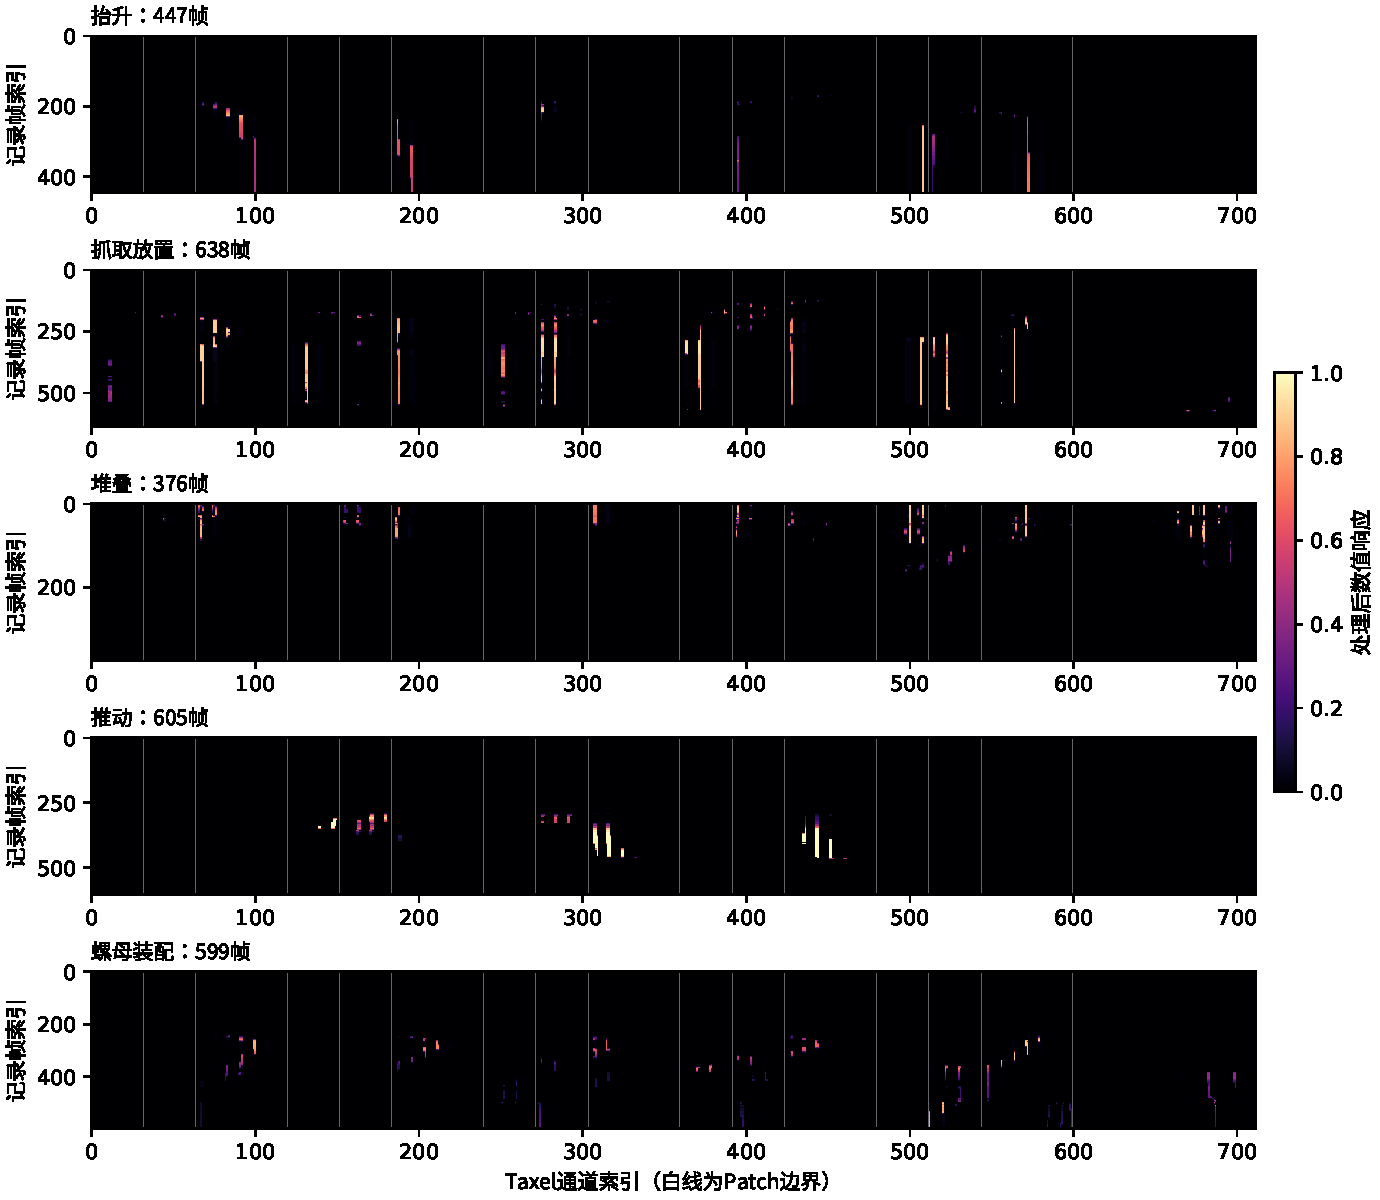
\includegraphics[width=0.96\textwidth]{figures/annotation_r2/historical_tactile_heatmaps.pdf}
  \caption{五条历史任务记录的处理后触觉热图（共用数值色标）}
  \label{fig:ch02_historical_heatmaps}
\end{figure}

表\ref{tab:ch02_episode_validation}中的五条触觉数组均为float32，满足$T\times712$的形状要求，所有元素有限、非负且存在非零响应。保存的float64时间戳相邻增量在浮点误差范围内为0.05~s，与20~Hz采样一致。触觉序列因此可以按记录索引分析接触响应的出现、持续和变化。

Push记录的非零比例为0.495\%，Stack为18.263\%。结合热图可以看到，推动记录仅在少量通道与时刻出现响应，堆叠记录的激活范围和持续阶段则更广。两者提示数据处理中应保留稀疏接触与较密集接触，而不以统一非零比例筛选所有任务。上述差异对应具体物体、轨迹及处理条件；每类一条记录用于展示观测特征，任务总体分布仍需按独立执行来源汇总。

五份NPZ同时保存tactile和sensor\_tactile，二者数值存在差异。本节按记录合同统一使用sensor\_tactile计算非零比例。两个字段的具体关系取决于相应版本的采样时刻与处理调用，现有检查尚未定位该差异的完整来源。

本节的证据范围为五条历史开发记录：其manifest及结果文件登记任务成功状态为True，Lift另有Strict严格轨迹回放记录。本文据保存数组分析触觉观测，未重新执行这些任务。历史记录与当前XML、曲面拟合和处理配置的完整版本对应关系为UNKNOWN；其独立来源还需结合初态分组（Root）与轨迹派生关系确定。相应统计分别保留帧数、执行记录及来源分组，以便后续数据审查。

上述检查确认了平台的模型、控制和观测接口，以及五条指定历史记录的数组有效性与基本采样关系。抓取候选如何转化为稳定操作，是下一章的研究问题；第四章则进一步检查这些执行记录的时序、来源及数据质量。真实触觉标定与跨域物理对应将在触觉重建的问题定义中统一讨论。

五类任务使用桌面、机器人及任务对象组成场景，初始条件由物体位姿、手部配置和目标区域确定。Lift以桌面物体为对象，依次接近、闭合、保持和抬升，任务接口按物体高度判断抬升结果；严格示教另检查尾段稳定性。PickPlace增加目标区域，抓持后运输、下降、释放并检查物体进入目标且手部离开。Stack在场景中增加支撑物，搬移目标物体到支撑面，释放后检查物体间接触与持续稳定。Push在桌面支撑下建立手物接触，反馈推动至目标区域，并检查位置、竖直范围与平面速度。NutAssembly场景包含待操作件与固定装配结构，抓持后调整姿态、运输和下降，按具体几何版本检查对准、插入及稳定状态。表中历史案例对应Sugar Box抬升、Tomato Soup Can搬移与推动、Stacking Ring堆叠及保留抓持命令的装配记录；各历史结果按自身manifest和版本解释，当前接口用于说明任务定义。

五类任务分别考察抓持后的垂直抬升、搬移与放置、物体堆叠、桌面推动以及螺母装配。图\ref{fig:ch02_historical_scenes}从上述五条记录的原始场景视频中提取首帧与末帧，展示物体、机械臂和灵巧手的相对位置及场景变化。起终帧用于说明各任务的操作对象与环境，任务结果仍按相应执行记录和验证条件判定。各任务的轨迹构建与执行条件在第三章进一步介绍。

\begin{figure}[p]
  \centering
  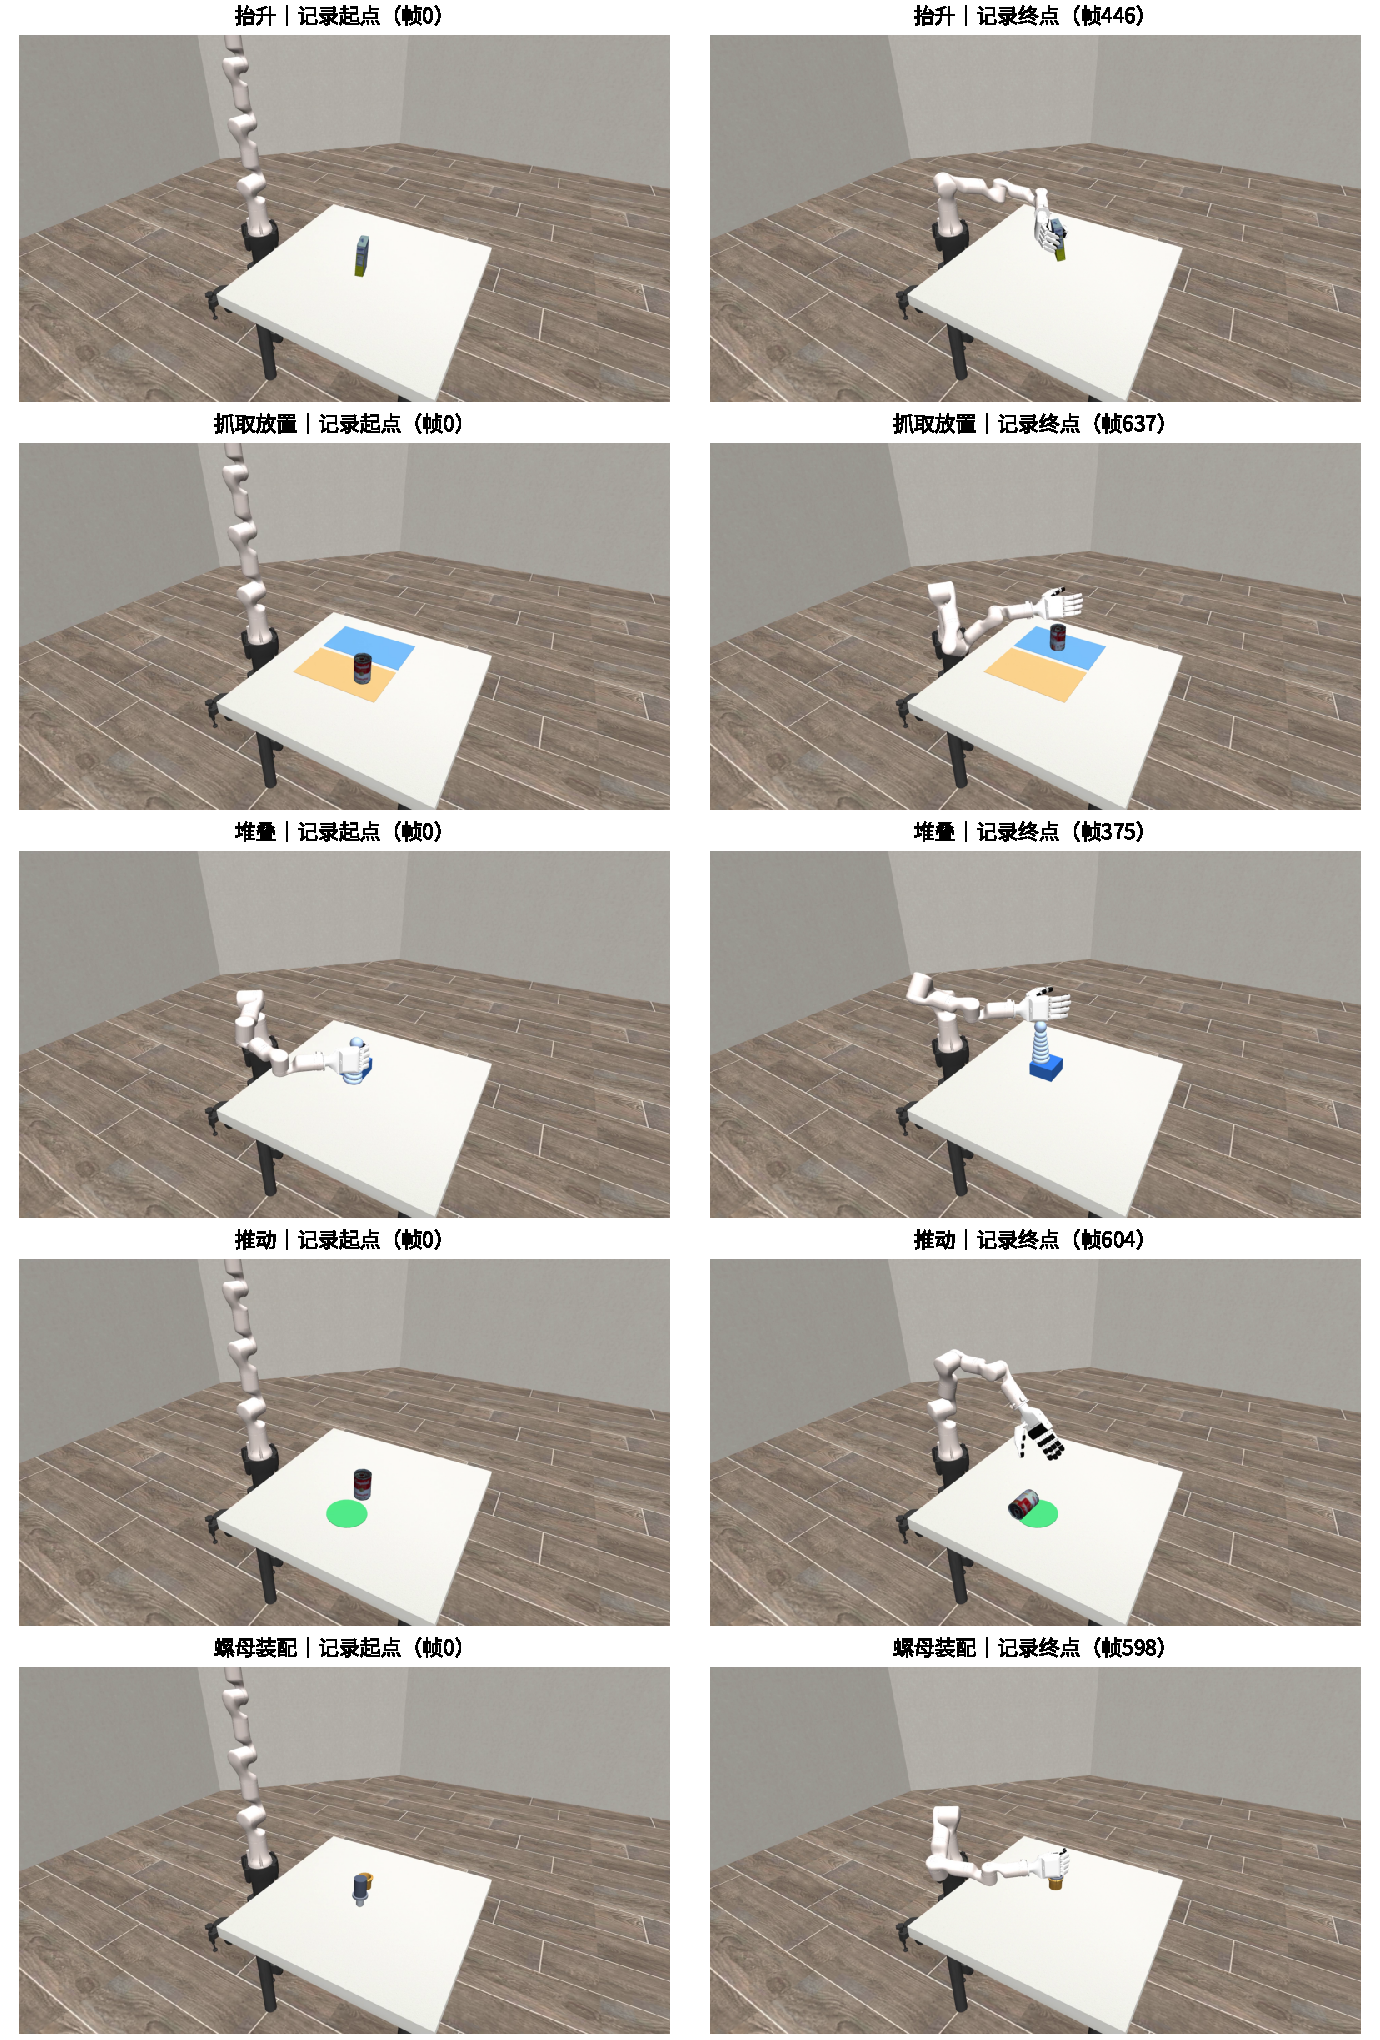
\includegraphics[width=0.92\textwidth,height=0.83\textheight,keepaspectratio]{figures/annotation_r2/historical_five_task_scenes.pdf}
  \caption{五任务历史仿真场景的记录起点与终点（原始视频帧）}
  \label{fig:ch02_historical_scenes}
\end{figure}

\section{本章小结}
\label{sec:platform_summary}

本章围绕多任务灵巧手操作的执行与感知需求，介绍了RM75B机械臂与途见科技灵巧手仿真平台的模型、控制、触觉、任务和记录接口。当前机械臂采用七个转动关节及位置执行器，手部采用十二个转动关节、六个固定腱和六个位置驱动通道。通过区分物理关节、传动坐标与控制通道，明确了欠驱动结构的实现范围，避免将历史命名中的推杆与当前机构混同。

控制过程区分关节目标或末端IK求解、底层位置伺服和物理积分，在指定配置下按20~Hz控制和1000~Hz积分执行。触觉阵列由皮肤STL派生，通过指节与指尖外壳拟合、手掌参数域投影及局部坐标构造形成16个Patch，再由712个原生touch感知区读取标量响应。死区、幂响应、时间滤波和邻域扩散进一步产生无量纲processed观测，其含义不同于经过标定的真实压力。

已有五条历史任务记录提供了触觉数组有限、非负和规则时间索引的功能证据，但与当前模型的完整版本一致性、独立Root关系及实物映射仍有限制。基于这些边界，下一章讨论如何将几何抓取候选转化为满足机械臂可达性、连续运动和任务要求的专家示教。

% !TeX root = ../thesis.tex
% TH-CH03-WRITE-V1: stage 3 draft; not compiled or frozen.
\chapter{面向灵巧手操作的抓取候选生成与专家示教构建}
\label{chap:grasp_demonstrations}

\section{抓取任务定义与总体流程}
\label{sec:grasp_task_pipeline}

第二章建立了机器人执行与触觉观测的仿真基础，但具有可控模型并不意味着能够直接生成有效操作轨迹。面对不同形状和摆放状态的物体，系统既要寻找手部可形成接触的构型，也要使该构型满足机械臂运动约束，并在实际动力学推进后保持物体。因此，本章从候选生成、机器人约束筛选、轨迹执行和质量验收四个层次展开：先寻找可抓取构型，再检验机械臂能否到达、操作能否执行以及所得轨迹是否满足示教要求。

抓取输入包括物体标识、表面采样及法向、初始位姿与任务条件。候选以物体坐标系下的手部平移、旋转和六维驱动比例表示，可记为
\begin{equation}
 \mathcal G=(\boldsymbol t_{oh},\boldsymbol R_{oh},\boldsymbol f,\mathcal C,\boldsymbol m),
 \qquad \boldsymbol f\in[0,1]^6,
 \label{eq:ch03_candidate}
\end{equation}
其中，$\boldsymbol t_{oh}\in\mathbb R^3$和$\boldsymbol R_{oh}\in SO(3)$描述物体坐标系下的手部目标，$\mathcal C$存储接触点、法向及距离，$\boldsymbol m$为候选质量和来源指标。驱动比例需进一步转换为具体执行器的控制范围，不等于十二个手部关节的独立角度。候选合同检查维度、旋转合法性和比例范围，这些检查只能保证表达有效，不能证明实际接触已经成立。

\begin{figure}[htbp]
  \centering
  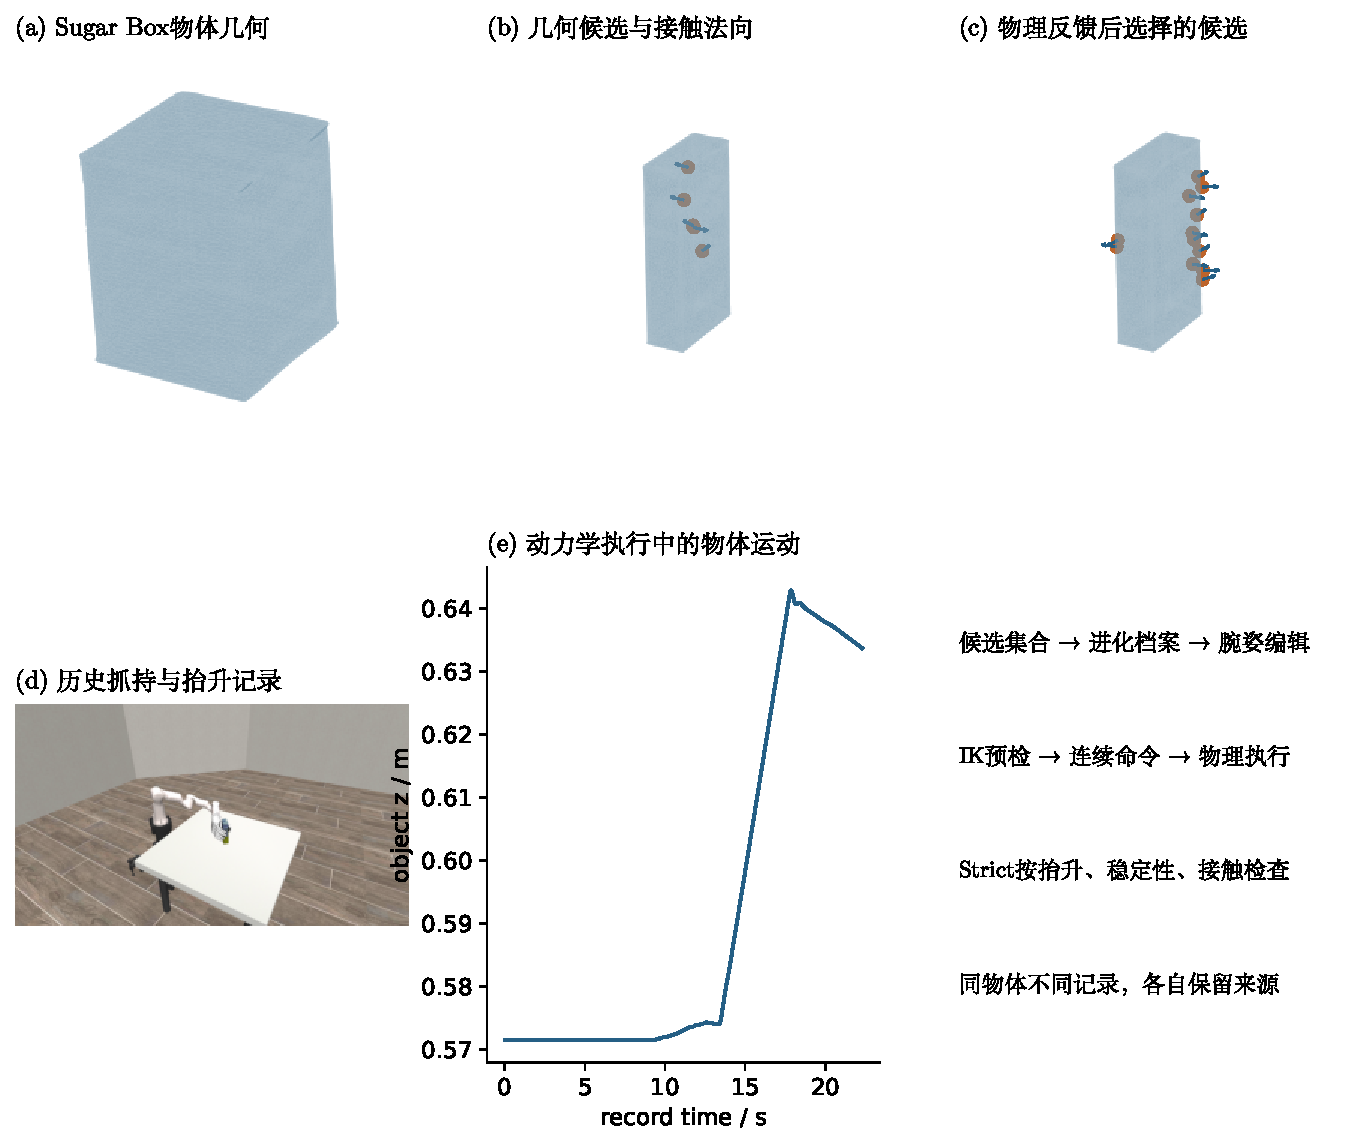
\includegraphics[width=0.97\textwidth]{figures/annotation_R2/grasp_evidence_pipeline.pdf}
  \caption{Sugar Box同物体案例的候选几何、执行反馈与示教构建证据}
 \label{fig:ch03_overall_pipeline}
\end{figure}

图\ref{fig:ch03_overall_pipeline}以Sugar Box贯穿候选几何与执行反馈：物体表面和保存的接触候选为几何评价提供输入，进化档案补充物理反馈，腕姿扩展与IK筛选再连接机械臂目标，连续命令进入实际执行与Strict回放。各画面保留原始记录身份，用于说明同一物体上的各环节，而非将不同候选拼成同一条优化轨迹。机器人约束筛选将对象相对目标转换为世界坐标下的机械臂末端目标，轨迹执行再连接接近、闭合、保持和后续操作。只有经过执行，才能获得状态、接触和物体运动等反馈；Strict质量验收进一步检查尾段稳定性。Lift提供抓持和抬升的基本案例，搬移与堆叠可在抓持前缀上构造任务后缀，推动和装配则需要额外的接触或姿态控制。五类任务共享示教数据合同，但不共享完全相同的物理执行逻辑。本章重点讨论示教如何形成，记录关联、数据转换与全量质量审计留在第四章。

\section{多来源抓取候选生成}
\label{sec:grasp_candidate_generation}

欠驱动手的关节并非独立受控，直接优化全部关节角可能偏离实际可执行构型。本文以六个驱动比例为手部参数，利用仿真采样拟合的皮肤点轨迹代理连接驱动与接触几何。该代理用于可微评价，其范围受采样和模型版本限制，最终行为仍需物理反馈检验。

GraspQP通过可微抓取质量评价支持候选优化\cite{zurbrugg2025graspqp}。本文调用其官方指标工厂，结合物体表面点、法向和手部代理构造接触评价。优化变量包括三维平移、六维旋转参数及六个驱动比例的logit，驱动比例通过sigmoid限制在有效区间。旋转参数在评价时恢复为旋转矩阵，从而避免直接优化九个任意矩阵元素。物体采样和手部皮肤点变换到同一坐标下后，程序按手指接触点组计算到物体的距离，并以软权重构造接触位置和法向。由此形成的接触集合用于官方质量指标计算，而不是把最近点距离本身当作力闭合证明。

单独优化抓取指标可能得到难以执行的构型，因此目标还加入接触距离、穿透、桌面距离、平移漂移和驱动耦合约束。接触距离项鼓励手部采样点接近物体；穿透和桌面项限制明显不合理的几何关系；漂移项抑制手部偏离初始种子过远；驱动耦合项约束部分手指比例的离散程度。各项具有不同归一化尺度与权重，其数值意义应结合实际实现解释。表\ref{tab:ch03_candidate_parameters}列出变量和约束的职责。这一适配使官方抓取指标能够作用于六驱动手的构型变量，后续仿真反馈进一步评价加载后的接触保持。

\begin{table}[htbp]
 \centering\small
 \caption{候选优化参数及约束的实际作用}
 \label{tab:ch03_candidate_parameters}
 \begin{tabular}{p{0.20\textwidth}p{0.25\textwidth}p{0.41\textwidth}}
 \hline
 项目 & 表达或输入 & 作用与边界\\
 \hline
 手部平移与旋转 & 三维平移、六维旋转参数 & 搜索对象相对手部位姿，输出合法旋转矩阵\\
 手部驱动 & 六维比例logit & 经sigmoid形成执行器比例，不独立控制全部关节\\
 接触几何 & 表面点、法向及距离 & 连接手部代理与物体几何评价\\
 官方抓取指标 & 接触集合与摩擦设置 & 提供几何抓取质量，不代替机器人执行\\
 附加几何约束 & 接触、穿透、桌面距离 & 排除部分明显不合理的候选\\
 漂移与驱动约束 & 种子平移及驱动比例 & 限制局部搜索偏移和驱动分散\\
 \hline
 \end{tabular}
\end{table}

几何候选进入DexEvolve-style细化阶段后，评价对象从接触构型扩展到执行行为。DexEvolve原研究采用进化优化获得多样且稳健的灵巧抓取\cite{zurbrugg2026dexevolve}，本文保留候选群体、变异、交叉和档案管理的组织思想，并针对六驱动手及现有仿真执行接口作适配。平移、旋转和驱动比例分别施加扰动，驱动变化限制在有效范围内；交叉则组合不同候选的位姿与手部配置。候选在执行前还可进行接触修正和去穿透处理，使搜索不仅依赖最初的几何种子。

物理反馈通过实际执行候选获得接触保持、物体相对漂移和扰动响应等指标，必要时使用MJWarp后端评价寿命相关目标。几何质量较高的构型仍可能在接近时偏离物体，或在加载后因接触方向不合适而失稳，因而物理反馈不能由静态接触分数完全替代。进化档案利用候选距离、新颖性及局部密度等信息保留不同构型，避免全部预算集中到近乎重复的局部解。档案按平移、旋转和驱动比例构成的嵌入计算候选距离；新候选若与最近档案项的距离小于新颖性阈值，仅在适应度更高时替换该项，否则作为新构型加入。父代选择再以局部密度修正适应度，减少拥挤邻域反复占用搜索预算；最终按适应度整理候选，供后续腕姿与机器人约束筛选。

\begin{figure}[htbp]
  \centering
  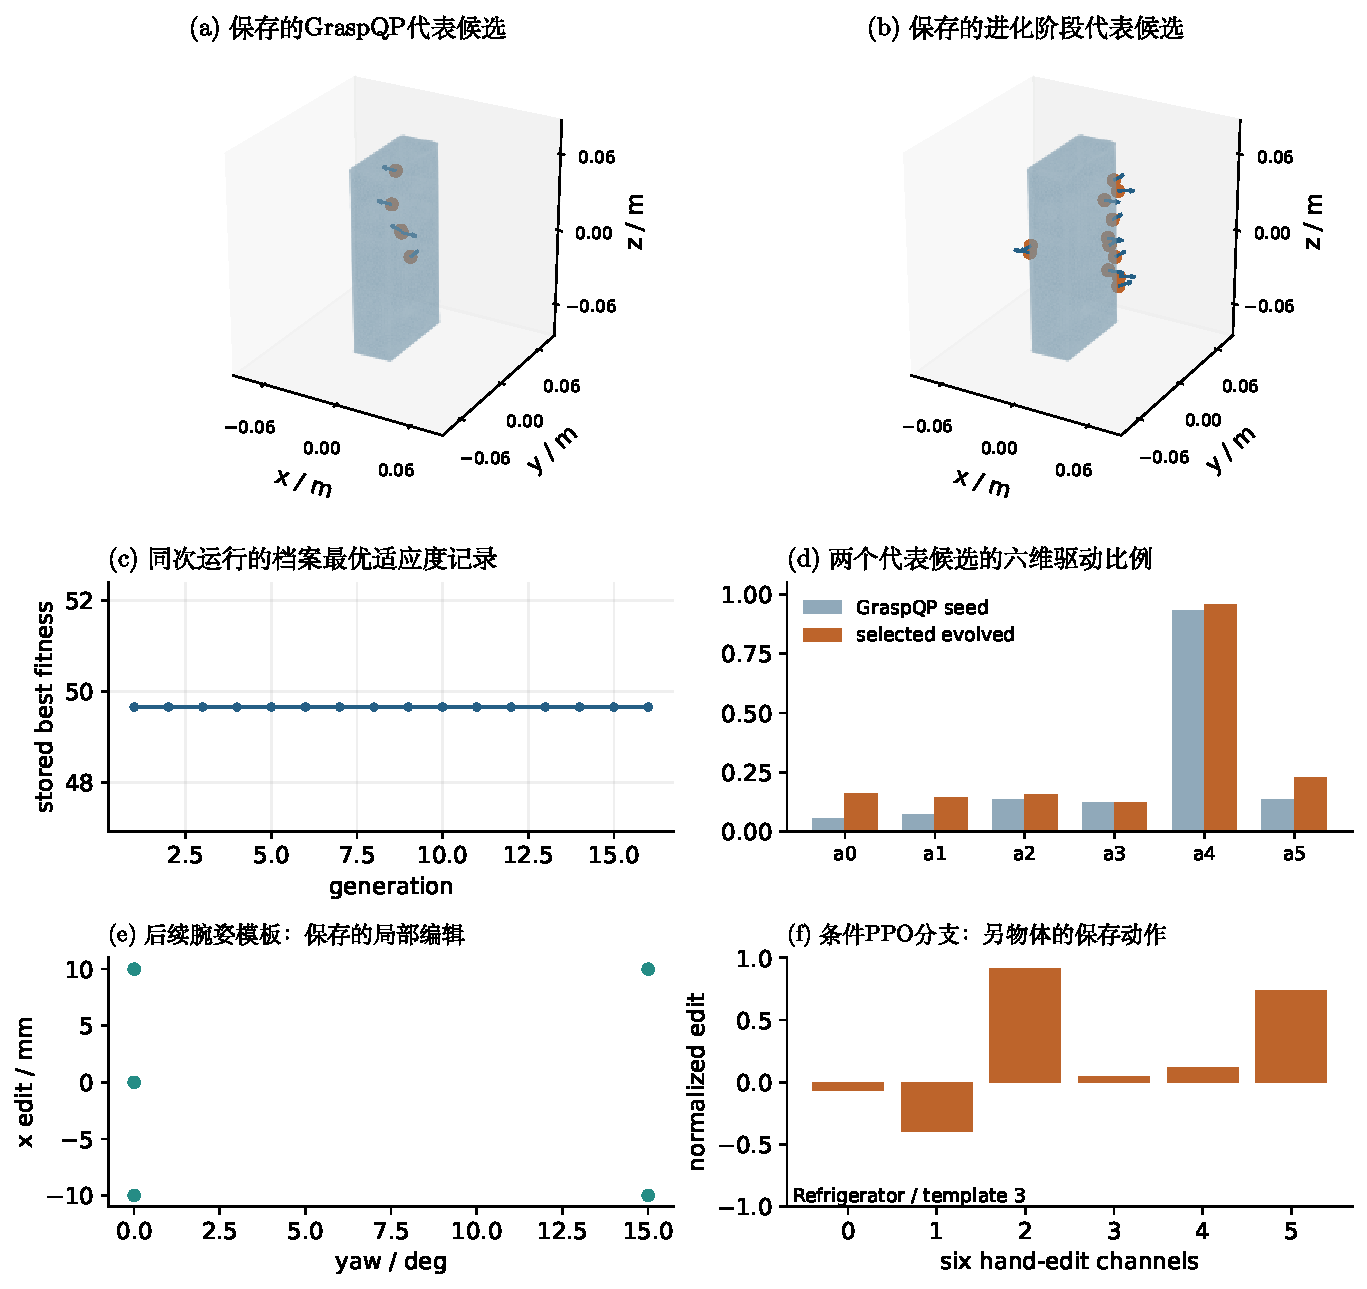
\includegraphics[width=0.97\textwidth]{figures/annotation_R2/candidate_geometry_feedback.pdf}
  \caption{代表候选、进化档案、腕姿模板与条件PPO分支的保存记录}
 \label{fig:ch03_candidate_sources}
\end{figure}

腕部姿态格点扩展（Wrist Lattice）用于搜索源候选附近更容易被机械臂到达的手腕位姿。它在源候选附近改变腕部平移和朝向，再以机器人逆运动学残差排序，保留可进一步执行的模板。当前默认集合包含39个格点，平移基本尺度为0.01~m，旋转基本尺度为$15^\circ$，并包含若干倍尺度的单轴旋转以及平移、旋转耦合编辑。该邻域保留源抓取附近的接触构型，同时为机械臂提供不同的腕部目标。39个格点是同一源候选的搜索编辑，预算按被评价的候选计量；搜索范围由所设平移与旋转尺度限定。

统一生成预算配置当前采用64个种子、150步GraspQP优化并执行12个候选；进化阶段使用24个初始个体、每代12个子代、16代，名义候选评价次数为216，随后向腕部扩展提供最多6个档案候选。这些是当前入口默认预算；历史批次及缓存复用的实际代价需另行区分。

图\ref{fig:ch03_candidate_sources}展示同次运行保存的几何候选、进化代表候选及档案最优适应度；接触点与法向直接来自候选文件，六维驱动比例反映不同抓持配置。MJWarp PPO仅作为条件性补充，在格点阶段未解决且仍有可用模板时进行模板选择与手部驱动编辑，图中另以Refrigerator记录展示该分支保存的模板选择与六维手部编辑，和Sugar Box的几何、进化与腕姿记录分别标识。历史Top100路由中存在2条RL\_SUCCESS记录，但这并不构成强化学习优于其他模块的消融证据。整体而言，可微指标提供几何方向，进化反馈检验物理行为，格点扩展处理机器人可达性，后续编辑尝试解决局部未完成案例。各模块依赖不同输入和预算，应分别说明作用，不能混合命名为一个新的原创抓取优化算法。

\section{基于可达性约束的抓取筛选}
\label{sec:grasp_reachability}

对象相对抓取只有在转换到机器人末端目标后，才能评价机械臂是否能够执行。设物体世界位姿为$(\boldsymbol R_{wo},\boldsymbol p_{wo})$，候选定义的手部目标为$(\boldsymbol R_{oh},\boldsymbol t_{oh})$，则目标手部姿态与末端姿态满足
\begin{equation}
 \begin{aligned}
 \boldsymbol p_{wh}&=\boldsymbol p_{wo}+\boldsymbol R_{wo}\boldsymbol t_{oh},\\
 \boldsymbol R_{wh}&=\boldsymbol R_{wo}\boldsymbol R_{oh},\qquad
 \boldsymbol R_{we}=\boldsymbol R_{wh}\boldsymbol R_{eh}^{\mathsf T}.
 \end{aligned}
 \label{eq:ch03_target_transform}
\end{equation}
其中，$\boldsymbol R_{eh}$为手部安装相对旋转，$w,o,h,e$分别表示世界、物体、候选手部参考与末端坐标。位置量单位为m，旋转无量纲。这里采用执行器接口中实际使用的安装参考，不能把STL局部原点任意替换为另一个掌心点后仍沿用同一公式。若缺少安装补偿，即使目标手部方向在几何上正确，机械臂实际跟踪方向也可能与之不同。

预抓取目标沿候选手部局部方向向外退让，当前默认距离为0.09~m；抓取目标则对应候选位置本身。筛选器按预抓取、抓取的顺序调用实际机械臂IK，在前一个求解结果上继续处理后一个目标。它同时记录位置残差、旋转残差与末端行程，用于区别几何合理但机器人难以到达的候选。检查过程中会保存并恢复环境状态、执行器控制量以及控制器历史目标，避免静态候选排序直接改变后续真正执行的起点。

当前排序器采用如下评分：
\begin{equation}
 S_{\mathrm{reach}}=20e_p^{\max}+0.6e_R^{\max}+0.08\ell,
 \label{eq:ch03_reachability_score}
\end{equation}
其中，$e_p^{\max}$和$e_R^{\max}$分别为两个目标上的最大位置与旋转残差，$\ell$为相应末端行程。三个系数是代码中的数值权重，用于产生排序，而非经过物理标定的统一距离单位。评分较小表示在该初值和求解配置下更易到达，不表示对应抓持必定稳定。静态排序还临时放宽目标速度约束，使残差更接近求解可达性的检查；真正执行时仍使用相应速度限制和平滑，不能将两条路径的跟踪结果视为相同。

模板构建依据执行配置保留位置误差不超过0.025~m、旋转误差不超过0.22~rad的候选。这两个容差属于当前生成执行层的筛选设置，不是第二章控制器内部更严格的迭代终止容差。满足筛选容差后，还需要根据腕部编辑幅度、源轨迹动态跟踪误差和候选评分确定执行顺序。这样既考虑静态残差，也保留对原有接触构型的偏好，避免搜索一开始就使用偏移很大的变体。

\begin{figure}[htbp]
  \centering
  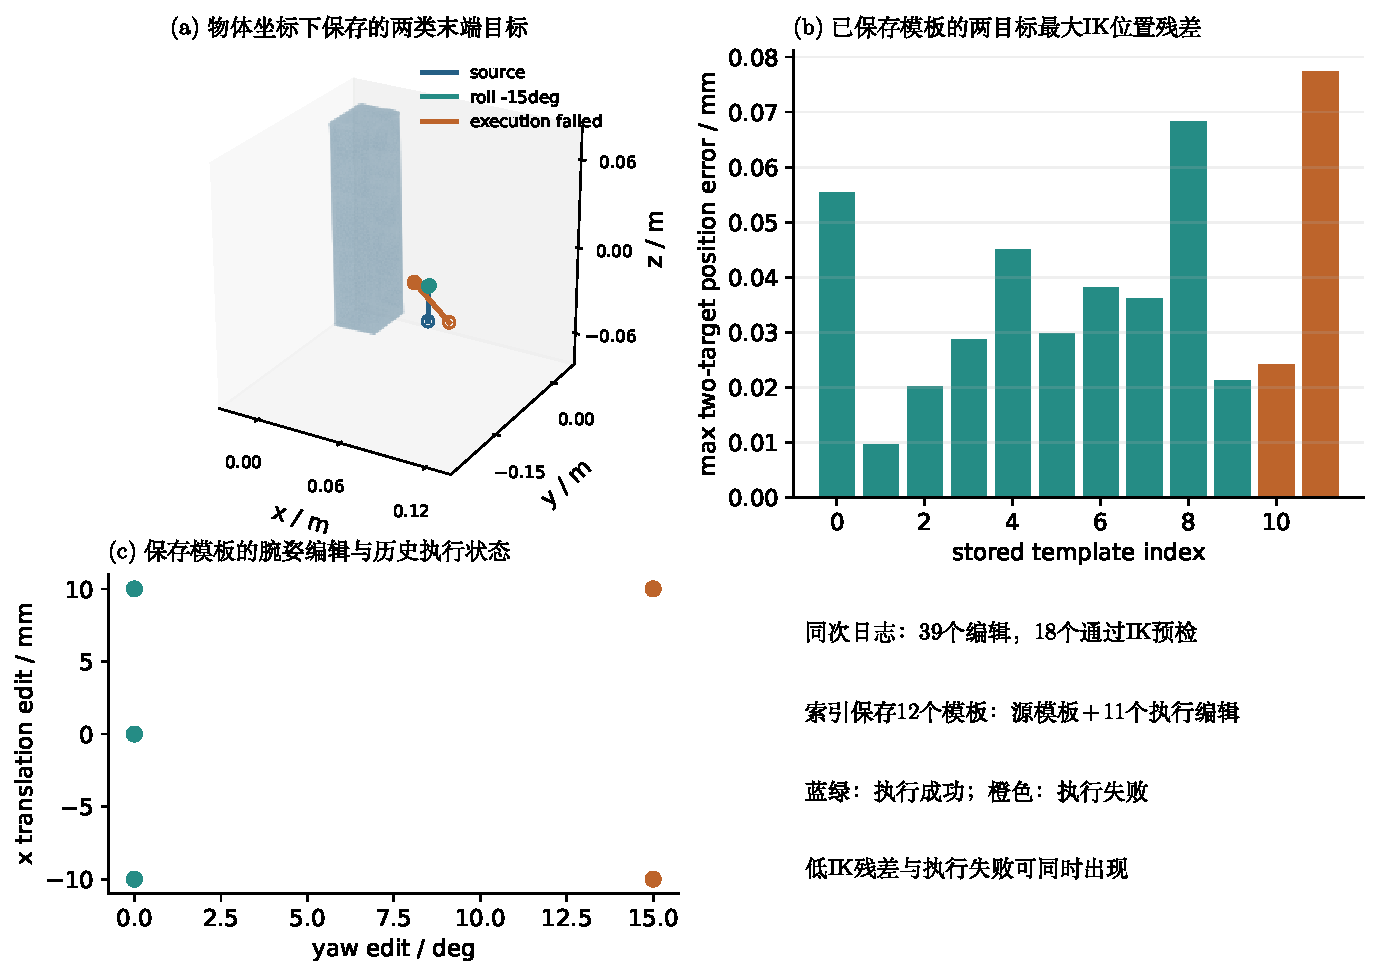
\includegraphics[width=0.97\textwidth]{figures/annotation_R2/wrist_recorded_targets.pdf}
  \caption{腕姿模板的保存目标、预检残差与历史执行结果}
 \label{fig:ch03_reachability}
\end{figure}

图\ref{fig:ch03_reachability}所示预检的作用范围需要明确：已核验实现主要覆盖预抓取与抓取两个目标，并没有据此证明完整Lift轨迹的每个路点都通过连续碰撞认证。两个端点均可达时，中间路径仍可能靠近桌面或改变IK分支；静态残差较小时，动态跟踪也可能因速度限制而产生更大误差。因此，筛选结果只决定候选是否值得进入执行，后续阶段仍需读取真实状态和接触结果，不能把它称为通用连续无碰撞规划器。

不同约束在流程中承担不同职责。候选优化中的桌面距离惩罚限制明显不合理的初始几何，任务迁移中的保守下降高度控制局部接近，执行过程监测接触和目标误差，Strict则对尾部桌面接触及稳定性作最终判断。这些机制相互补充，但不应合并为一个未经实现的全局碰撞约束。对失败也应保留层次：无有效候选、静态IK残差过大、动态接近偏差、闭合后缺少对向接触和抬升失稳对应不同问题。只有明确失败发生在哪一层，才能避免把所有失败归因于抓取几何质量。

局部搜索还受预算限制。模板构建对可执行候选排序后，只运行有限数量的完整尝试，并可优先复用已有参考。这有助于控制批量生成代价，但意味着最终保留下来的模板不等于全部可达候选，也不构成对整个抓取空间的穷举。本文将这种筛选视为面向具体机器人和源候选的约束连接环节，其有效范围由后续实际执行与验收结果共同确定。

图\ref{fig:ch03_reachability}将腕姿编辑与已保存的预检结果对应。同次日志登记39个编辑中18个通过预抓取及抓取两目标检查，模板索引保存其中12个执行或复用模板。图中的残差是两目标误差的最大值；橙色模板虽然预检残差较小，实际执行仍失败。这说明腕姿可达性只解决目标求解条件，后续接触保持仍需通过物理执行检查。被预检排除候选的逐姿态状态未保存在该索引中，因此图中以原日志给出筛选规模，不另画未经记录的不可达姿态。

\section{连续逆运动学与轨迹验证}
\label{sec:grasp_trajectory_verification}

通过静态筛选后，候选还需要变成从机器人当前状态出发的连续命令。执行器将目标分解为稳定初态、过渡、预抓取、接近、闭合、保持、抬升和验证等阶段，每个阶段具有目标末端位姿、手部命令和控制步数。分段组织的目的不是人为把操作拆成互不相关的动作，而是在接触建立前后采用不同目标，并保留阶段边界上的误差及接触信息。前一阶段输出的实际状态构成后一阶段的起点，因而不能只保存各阶段名义目标而忽略执行结果。

对单段执行，位置和手部控制量在起点与终点之间插值，姿态采用四元数SLERP。当启用平滑选项时，归一化进度经过三次映射后再用于插值：
\begin{equation}
 \begin{aligned}
 \bar u&=3u^2-2u^3,\qquad u\in[0,1],\\
 \boldsymbol p(u)&=(1-\bar u)\boldsymbol p_0+\bar u\boldsymbol p_1,\\
 \boldsymbol a_h(u)&=(1-\bar u)\boldsymbol a_{h,0}+\bar u\boldsymbol a_{h,1}.
 \end{aligned}
 \label{eq:ch03_segment_interpolation}
\end{equation}
其中，$\boldsymbol a_h$为六个手部执行器的位置命令；关闭平滑时直接使用$u$。该映射使参数曲线端点斜率为零，能够缓和相邻阶段的名义速度突变，但并不保证实际物体速度也为零。接触力、手部加载和关节伺服仍影响动力学结果，不能把插值平滑等同于抓持稳定。

末端目标按控制周期输入第二章所述IK控制器，控制器以已有目标和状态作为后续求解的参考，并限制关节更新与目标速度。这里不重复DLS推导，而强调其在连续执行中的角色：目标位姿是上层轨迹要求，实际关节状态由受限求解、执行器伺服和物理推进共同产生。执行过程保存接近位置和旋转残差，若超出执行配置允许范围，则停止将该候选视为有效接近。对接触建立后的阶段，还需要检查拇指对向皮肤接触、物体抬升和保持状态，防止仅凭完成命令序列就认定任务成功。

\begin{figure}[htbp]
  \centering
  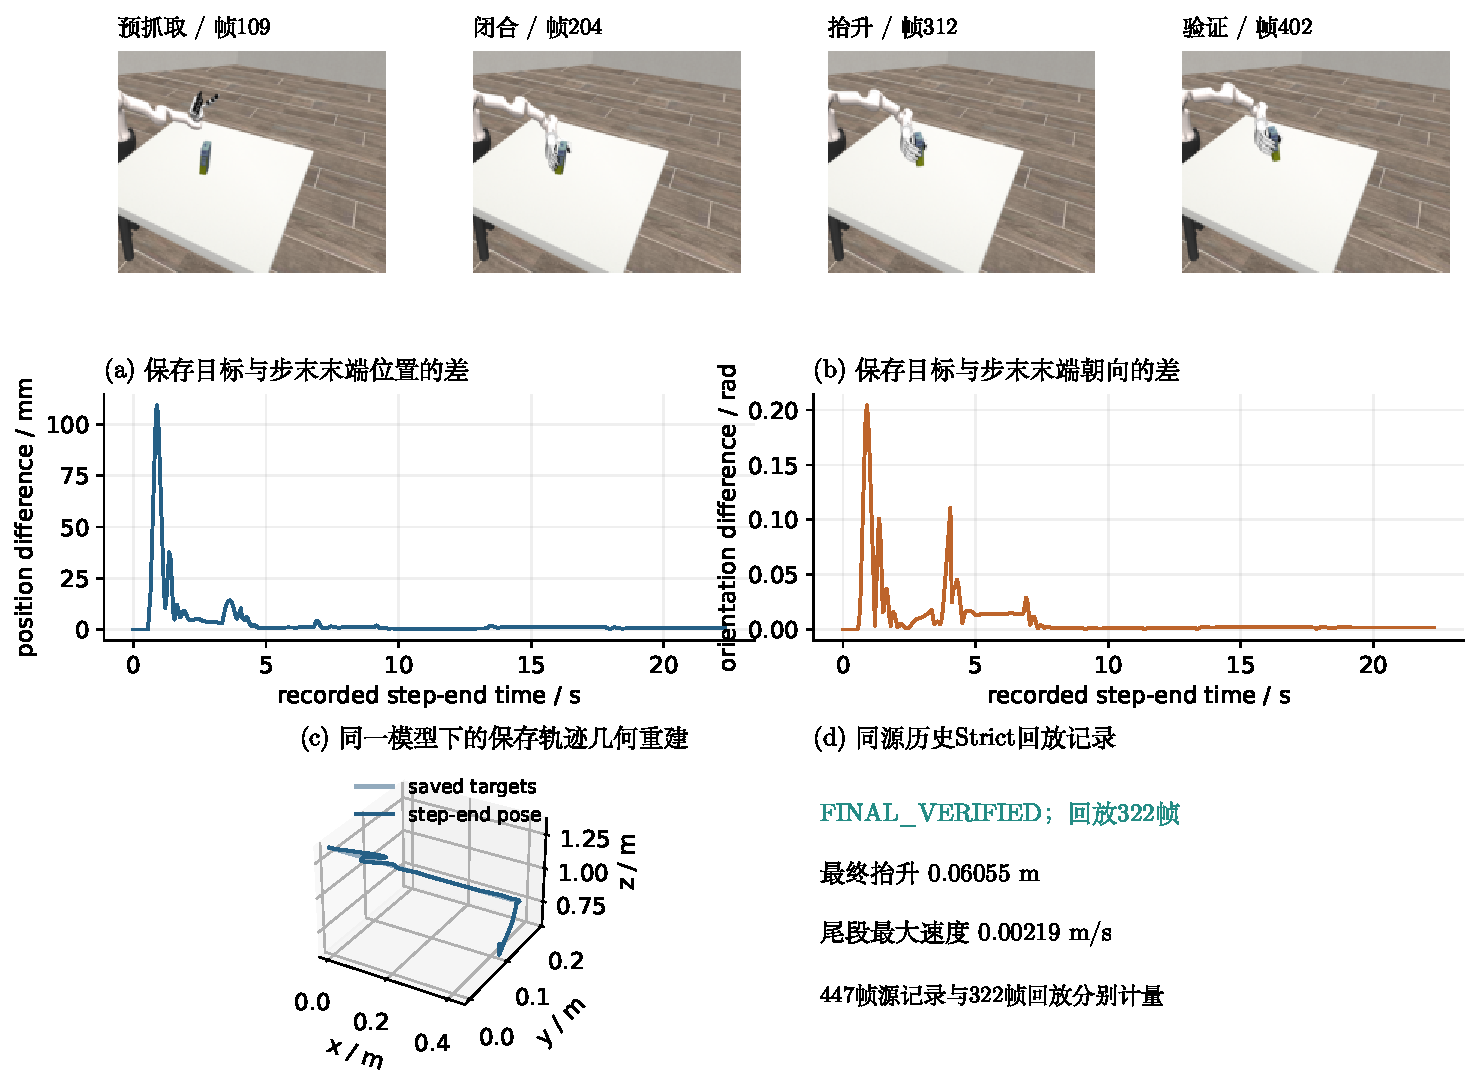
\includegraphics[width=0.97\textwidth]{figures/annotation_R2/recorded_tracking_strict.pdf}
  \caption{保存模型与关节状态的末端跟踪重建及同源历史Strict结果}
 \label{fig:ch03_strict_replay}
\end{figure}

图\ref{fig:ch03_recorded_trajectory}给出一条Sugar Box历史抬升记录中的命令与执行反馈。阶段边界直接取自保存的stage字段，三幅图共用记录时间轴。关节位置命令描述控制器要求，物体高度和接触数则反映实际执行过程：闭合与保持阶段建立接触，抬升阶段物体高度随之变化。将这些记录放在同一时间轴上，可以检查操作阶段与物体运动是否相衔接，并定位接触建立或丢失的时刻。该例用于展示历史执行过程，Strict质量仍按相应验证记录及其阈值判定。

\begin{figure}[htbp]
  \centering
  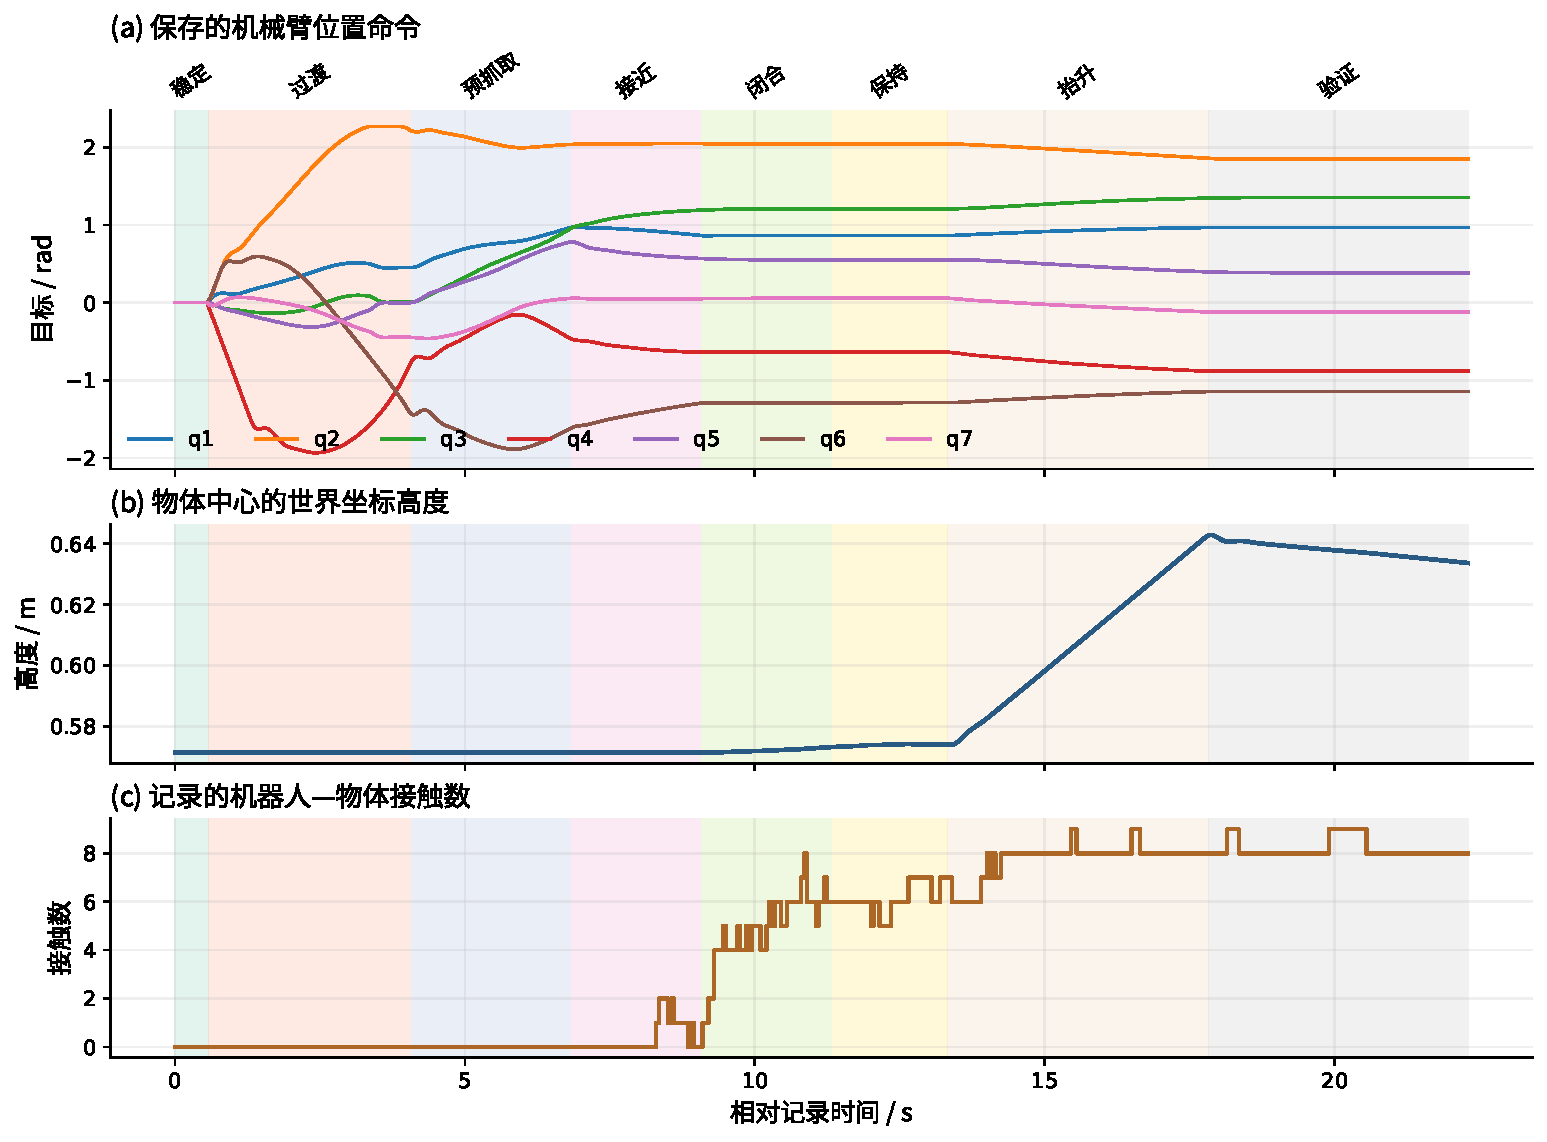
\includegraphics[width=0.96\textwidth]{figures/annotation_batch2/historical_lift_trajectory.pdf}
  \caption{Sugar Box历史抬升示教的位置命令、物体高度与接触反馈}
  \label{fig:ch03_recorded_trajectory}
\end{figure}

图\ref{fig:ch03_strict_replay}进一步利用另一条开发记录保存的模型快照与447帧关节状态，作静态正运动学重建。位置差为步末末端位置与同一行保存IK目标之差的范数，朝向差取四元数对应的最短旋转角；它们包含目标滤波、伺服和动力学跟踪影响，区别于IK求解器内部残差。关键阶段画面也仅恢复保存姿态。图中同源历史Strict文件登记322帧回放为FINAL\_VERIFIED，源序列与回放帧数分别标注，未在本次绘图中重新执行验证。

已有普通Replay接口主要检查控制序列能否回放，以及尾段任务成功比例。其成功条件要求最后一个尾段标记为成功，且尾段成功比例至少为0.8。该接口并未完整表达严格示教所需的稳定性条件，因此另外采用图\ref{fig:ch03_strict_replay}所示的Strict Replay。在对应仿真环境中重放实际低层控制序列后，Strict同时检查抬升、速度、角速度、皮肤接触和环境碰撞等指标，当前final配置见表\ref{tab:ch03_strict_thresholds}。

\begin{table}[htbp]
 \centering\small
 \caption{当前final配置的Strict Replay验收条件}
 \label{tab:ch03_strict_thresholds}
 \begin{tabular}{p{0.39\textwidth}p{0.17\textwidth}p{0.30\textwidth}}
 \hline
 指标 & 阈值 & 判定范围\\
 \hline
 最终及尾段最小抬升 & $\geq0.055$~m & 二者均需满足\\
 物体线速度 & $\leq0.10$~m/s & 尾段最大值\\
 物体角速度 & $\leq0.10$~rad/s & 尾段最大值\\
 皮肤接触、抓持比例 & 均$\geq0.80$ & 尾段统计\\
 机器人与桌面接触比例 & $\leq0$ & 尾段统计\\
 最大穿透 & $\leq0.003$~m & 尾段最大值\\
 验证尾段、额外保持 & 20步、12步 & 当前配置参数\\
 \hline
 \end{tabular}
\end{table}

Strict中的皮肤接触与抓持具有具体语义，不将任意机器人连杆碰撞当作有效指面抓持。全程最大穿透和尾段最大穿透虽然都被记录，实际最终布尔条件使用后者；若将全程记录量误写为硬门槛，就会改变原验证协议。最终及尾段最小抬升同时受限，也意味着物体曾短暂达到目标高度并不足够，尾段仍需满足要求。速度和角速度限制进一步区分持续承载与明显滑移、旋转等不稳定状态，桌面接触条件则避免利用环境支撑冒充稳定悬持。

验收状态由实际profile及布尔结果共同确定，final配置通过时记为FINAL\_VERIFIED，否则为FINAL\_REJECTED。生成过程中的某个变量即使名为strict\_execution，也不能替代该最终状态。类似地，物理执行返回success与严格回放通过是不同证据，候选档案、模板清单和示教导出需要保留验证层级。导出入口默认先进行final检查，诊断性允许未验证轨迹的开关不能作为正式质量保证。

轨迹重放还必须使用正确的动作语义。旧生成记录中的action可以是末端IK指令，ctrl则保存实际施加的机械臂七通道与手部六通道位置命令。二者均可能为十三维，但直接用前者替代后者会改变回放问题。记录器保存的关节状态、对象姿态和控制量有助于检查这种对应，完整时间关联则在第四章讨论。Strict通过只说明给定模型、初态、控制序列及阈值下的结果，不认证任意后续模型版本均能复现，也不把同一轨迹的后缀当成新的独立专家示教。

算法\ref{alg:grasp_demonstration_pipeline}归纳候选到示教的分层处理关系，各任务仍采用其专属执行与验证条件，不将这一归纳视为所有任务均调用同一实现。
\begin{algorithm}[H]
\small
\caption{抓取候选筛选与专家示教验证流程}\label{alg:grasp_demonstration_pipeline}
\KwIn{物体与资产版本、初始条件、候选来源及任务配置}
\KwOut{示教记录、任务结果及适用的验证状态}
利用已有候选来源获得几何候选，保留来源与评分\;
\ForEach{有限预算内的候选及局部腕姿编辑}{
将物体相对目标转换至机器人末端目标，补偿安装变换\;
求解预抓取与抓取目标IK，检查残差和关节条件\;
\If{未通过当前层的筛选}{登记失败类别，继续下一候选\;}
按任务配置构造分段目标并执行，记录状态、低层命令与结果\;
对要求独立Strict检查的轨迹，依据对应配置执行回放与联合检查\;
分别登记任务结果和验证状态，保留失败记录及来源\;
}
按任务专属条件整理专家示教，不以单目标可达替代完整执行检查\;
\end{algorithm}

\section{多任务专家示教生成}
\label{sec:multitask_demonstration}

多任务示教共享候选来源、控制序列、对象状态和阶段信息等记录合同，但采用不同控制逻辑。Lift提供基本抓持案例，其他任务依据操作目标构造后续过程，并以实际物体状态而非执行器目标判断结果。主要阶段见表\ref{tab:ch03_task_stages}。

Lift执行从稳定初态开始，经过过渡和预抓取接近，在close阶段逐步建立手部闭合命令，在hold阶段检查和维持接触，然后抬升并进入verify。接近阶段需要机械臂跟踪手部目标，接触阶段则要求驱动命令与物体几何形成有效加载；两者失败不能用同一几何指标解释。完整阶段记录让后续能够判断失败发生在物体接触之前还是加载之后，也为其他任务选择可用抓持前缀提供依据。

PickPlace以源抓持为基础，增加抬高避让、横向运输、下降、释放、撤离及任务验证。转移时既要保留物体初态与抓持目标的关系，也要考虑手部和桌面之间的几何余量。当前实现存在恢复已验证Lift终态并复用原前缀的路径，也存在从reset重新执行的选择。前者可以避免重复执行中的数值漂移，却不能被描述成整个拼接序列在该次运行中全部重新产生。对示教而言，前缀来源及衔接方式应明确保留，不能只凭拼接后数组长度判断物理连续性。

后续在线记录工作对原有前缀复用分支作了区分，重新执行时保留实际观测和控制，不将历史Lift触觉直接复制成新采集结果。这项修复说明示教生成与数据保存之间存在接口约束：任务控制完成和记录正确并不是同一个条件。本节只交代两种生成路径及其限制，完整模态关联与修复验收由第四章展开，不把修复后的合同回填为全部历史文件都已具备的属性。

\begin{table}[htbp]
 \centering\small
 \caption{五类任务的示教阶段与主要执行约束}
 \label{tab:ch03_task_stages}
 \begin{tabular}{p{0.15\textwidth}p{0.42\textwidth}p{0.29\textwidth}}
 \hline
 任务 & 主要阶段 & 执行重点\\
 \hline
 Lift & settle、transit、pregrasp、approach、close、hold、lift、verify & 接近跟踪、对向接触与抬升保持\\
 PickPlace & 抓持前缀、clear、transport、descend、release、retreat、task\_verify & 来源保持、安全下降及释放后目标状态\\
 Stack & 抓取、目标定位、运输下降、释放、稳定性评价 & 被操作物与支撑物关系\\
 Push & 接触接近、接触检测、反馈推动、目标评价 & 持续推动与物体实际位移\\
 NutAssembly & Bolt抓持、姿态伺服、平移、下降、装配评价 & 载荷保持、朝向与装配几何\\
 \hline
 \end{tabular}
\end{table}

Stack除被操作物之外还需要支撑物的状态。源抓持能够提供手与物体的相对关系，但堆叠目标必须根据支撑物位置、物体尺寸和下降范围进一步确定。任务后缀通过运输、下降和释放形成支撑关系，再检查物体是否稳定放置。并非每个物体都适合当前堆叠定义，因此已有批次先选取task-valid对象域。对这一筛选应保留来源，不能将限定物体域上的成功比例写成对任意物体的覆盖能力。

图\ref{fig:ch03_task_transfer}按各源序列保存的阶段选取中点画面。Lift展示抓持前缀与抬升，PickPlace展示抓持后的运输和释放；Stack所示记录从已有抓持状态后的运输阶段开始，支撑物贯穿下降和释放过程。推动与装配分别展示持续接触和抓持后姿态调整、下降的不同操作要求。

\begin{figure}[htbp]
  \centering
  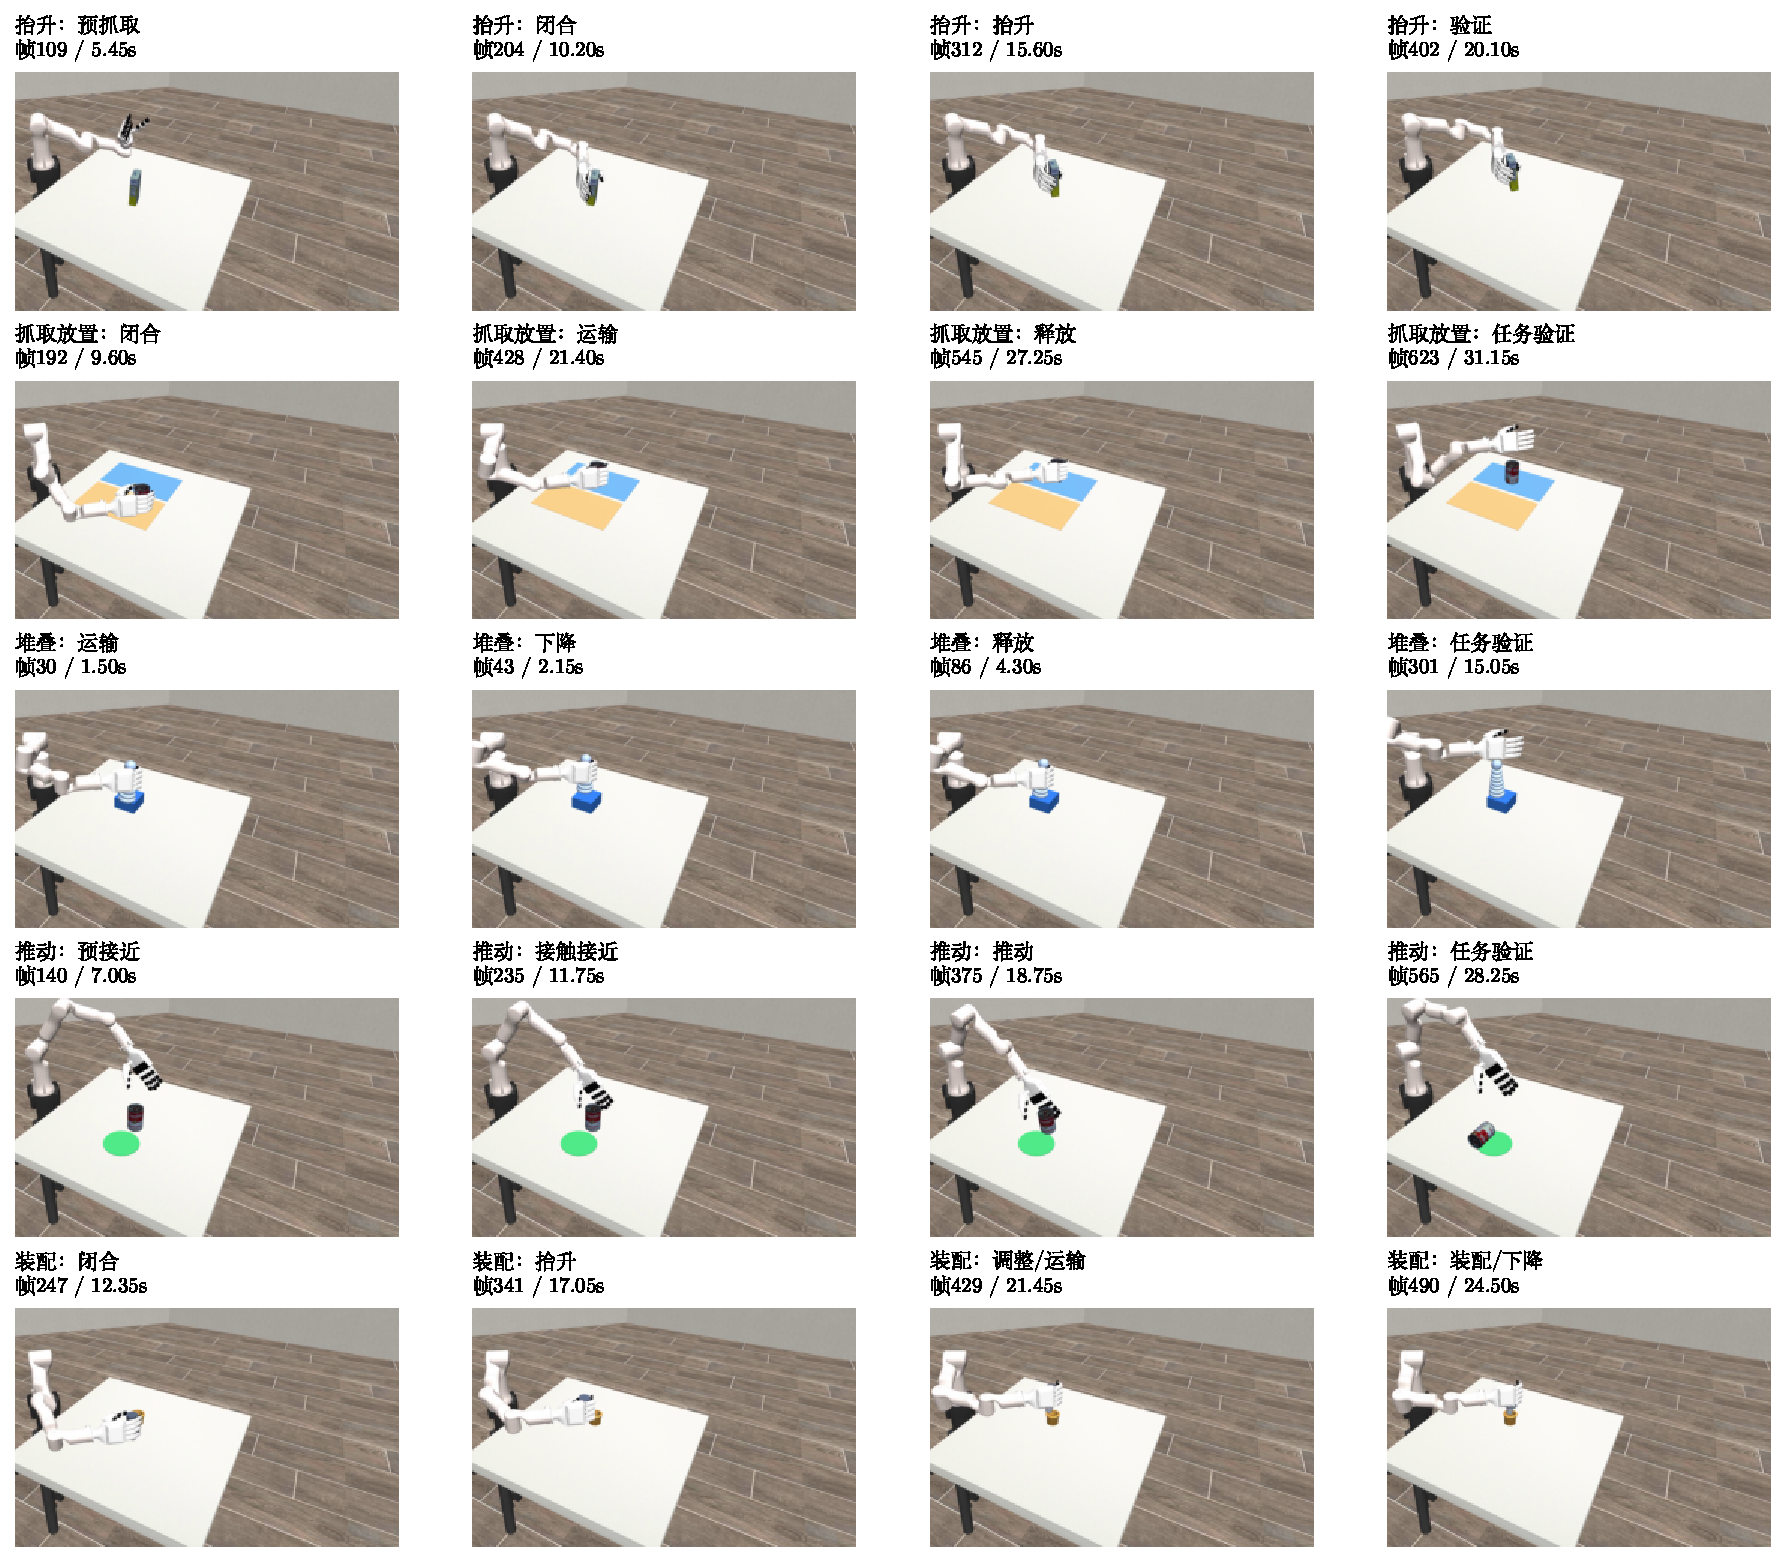
\includegraphics[width=0.97\textwidth]{figures/annotation_R2/five_task_phase_records.pdf}
  \caption{五类历史专家示教的实际阶段画面（按保存阶段中点选帧）}
 \label{fig:ch03_task_transfer}
\end{figure}

Push通过手掌或手指几何建立推动接触，并依据物体当前状态与目标位置的偏差反馈推进。其执行验证同时检查接触建立和物体实际位移，触觉用于描述推动阶段的接触响应。图\ref{fig:ch03_task_transfer}给出预接近、接触接近、推动及任务验证的历史画面，展示桌面支撑条件下的持续接触控制。

NutAssembly包含抓持Bolt、姿态伺服、平移、下降与装配结果评价。抓持阶段的细小偏差可能使物体倾斜，在后续下降前就丢失可用接触，因此不能把所有装配失败都归因于对孔精度。现有实现保留手部控制策略对承载过程的影响，也保留旧variant与后续几何版本不兼容的记录。局部成功可以用于分析某个控制条件是否值得保留，却不足以说明不同初态都能稳定装配，更不能把旧版本成功清单当成当前几何的最终验收。

上述专家示教通过候选、规划和任务反馈控制生成\cite{mandlekar2022demonstrations,mandlekar2023mimicgen}。每条轨迹随同保存任务条件、执行结果和验证状态，使后续使用者能够区分成功示例、失败示例与严格回放合格轨迹。第四章进一步讨论这些记录的时序配对、格式转换和来源追踪。

\section{抓取及示教质量实验}
\label{sec:grasp_quality_experiments}

本节依次考察候选路由能否提供可用模板、局部扰动示教是否满足Strict条件，以及执行失败发生在哪些阶段。表\ref{tab:ch03_historical_batches}先集中列明历史批量记录的来源与统计单位，再用具有源数组和验证文件的具体案例分析接触保持与轨迹质量。

Lift的100个对象标识中，98条由格点模板路由登记成功，2条由强化学习编辑路由登记成功，表明局部腕姿搜索是该批次主要的模板来源。PickPlace与Push分别登记100条SUCCESS，其缓存身份在表中单列；Stack在task-valid对象域中记录43条成功与5条失败；NutAssembly按variant记录100条成功。这些结果描述分级流程的产物覆盖，模块独立贡献则需要另设共同预算和初态的比较。

\begin{table}[htbp]
 \centering\small
 \caption{历史批量路由与任务记录及其统计限制}
 \label{tab:ch03_historical_batches}
 \begin{tabular}{p{0.16\textwidth}p{0.12\textwidth}p{0.30\textwidth}p{0.28\textwidth}}
 \hline
 任务或阶段 & 记录数 & 历史状态 & 解释限制\\
 \hline
 Lift候选路由 & 100 & 98 LATTICE\_SUCCESS，2 RL\_SUCCESS & 不是100条\newline\mbox{FINAL\_VERIFIED}\\
 PickPlace & 100 & 100 SUCCESS & 全部cached\\
 Stack & 48 & 43 SUCCESS，5 FAILED & 仅task-valid对象域\\
 Push & 100 & 100 SUCCESS & 98条cached\\
 NutAssembly & 100 & 100 SUCCESS & variant记录，非100个独立物体\\
 \hline
 \end{tabular}
\end{table}

上述批量表统一保留历史身份：Top100登记的18项源码Hash中，核对时12项相同、5项不同、1项对应文件缺失；cached表示复用结果，variant表示几何或配置变体，均以原记录单位计量。以下Sugar Box局部扰动与90次历史尝试另按各自来源和判据分析，避免以不同批次组成统一成功率。

局部扰动示教采用Sugar Box的10条既有记录。每份均有对应manifest，包含不同seed及不同NPZ Hash，源文件Hash与原审计登记一致，10份历史Strict结果均为FINAL\_VERIFIED。表\ref{tab:ch03_sugar_strict}列出其最终抬升和尾段角速度，展示严格通过并不只依赖数组中的成功标签。各记录使用同一物体和相近源抓取，历史审计记载不同初始位置的两两距离为0.707--2.828~mm，属于局部条件变化，不是大范围工作空间或跨物体泛化测试。

\begin{table}[htbp]
 \centering\small
 \caption{Sugar Box局部扰动示教的历史Strict结果}
 \label{tab:ch03_sugar_strict}
 \begin{tabular}{rrrrl}
 \hline
 序号 & seed & 最终抬升（m） & 尾段最大角速度（rad/s） & 验收状态\\
 \hline
 1 & 18011 & 0.06431 & 0.04049 & FINAL\_VERIFIED\\
 2 & 18012 & 0.06304 & 0.00324 & FINAL\_VERIFIED\\
 3 & 18013 & 0.06304 & 0.00303 & FINAL\_VERIFIED\\
 4 & 18014 & 0.06299 & 0.00311 & FINAL\_VERIFIED\\
 5 & 18015 & 0.06115 & 0.05234 & FINAL\_VERIFIED\\
 6 & 18016 & 0.06387 & 0.04748 & FINAL\_VERIFIED\\
 7 & 18017 & 0.06265 & 0.00602 & FINAL\_VERIFIED\\
 8 & 18018 & 0.06420 & 0.00428 & FINAL\_VERIFIED\\
 9 & 18019 & 0.06400 & 0.04943 & FINAL\_VERIFIED\\
 10 & 18020 & 0.06304 & 0.00346 & FINAL\_VERIFIED\\
 \hline
 \end{tabular}
\end{table}

10条序列均在源模板附近通过历史Strict条件，说明该抓取在所记录的小范围初态变化下能够保持承载与尾段稳定。该结果适用于同物体、相近源抓取的局部条件，评价重点是示教质量而非算法间排名。

\begin{table}[htbp]
 \centering\small
 \caption{历史90次扰动尝试的汇总分类}
 \label{tab:ch03_generation_failures}
 \begin{tabular}{lrp{0.51\textwidth}}
 \hline
 汇总类别 & 次数 & 统计解释\\
 \hline
 接受 & 46 & 历史生成汇总中的接受结果\\
 Strict不稳定 & 18 & 进入严格检查后未满足稳定条件\\
 Lift失败 & 26 & 未形成相应成功抬升轨迹\\
 \hline
 \end{tabular}
\end{table}

表\ref{tab:ch03_generation_failures}的历史报告按90次尝试登记46条接受、18条Strict不稳定和26条Lift失败。Lift失败对应未完成成功抬升，Strict不稳定则说明完成前序执行后仍可能在尾段速度、角速度或接触条件上不合格。两层淘汰分别对应承载建立和稳定示教的不同要求。该表为历史汇总证据；附加诊断可能重叠，且与前述局部示教存在来源重用，故保留原分母分别报告。

典型Lift案例的历史Strict结果中，最终抬升为0.0608926~m，尾段接触和抓持比例均为1，支持在该条件下持续承载的解释。NutAssembly则保留原始执行失败、降低抓点后仍失败、在降低抓点基础上保留hold抓持命令后单例成功的对照。该结果提示问题可能在装配之前的抓持保持阶段已经形成，而非只与末端对准有关；但它只是局部控制条件的对照，不能解释为跨seed稳定提升。图\ref{fig:ch03_examples}直接对照三条保存序列的物体高度、接触数和阶段。失败记录没有视频，图中使用其自身数组；不同记录长度与阶段进度分别呈现，便于检查抓持、运输和装配阶段的接触变化。

\begin{figure}[htbp]
\centering
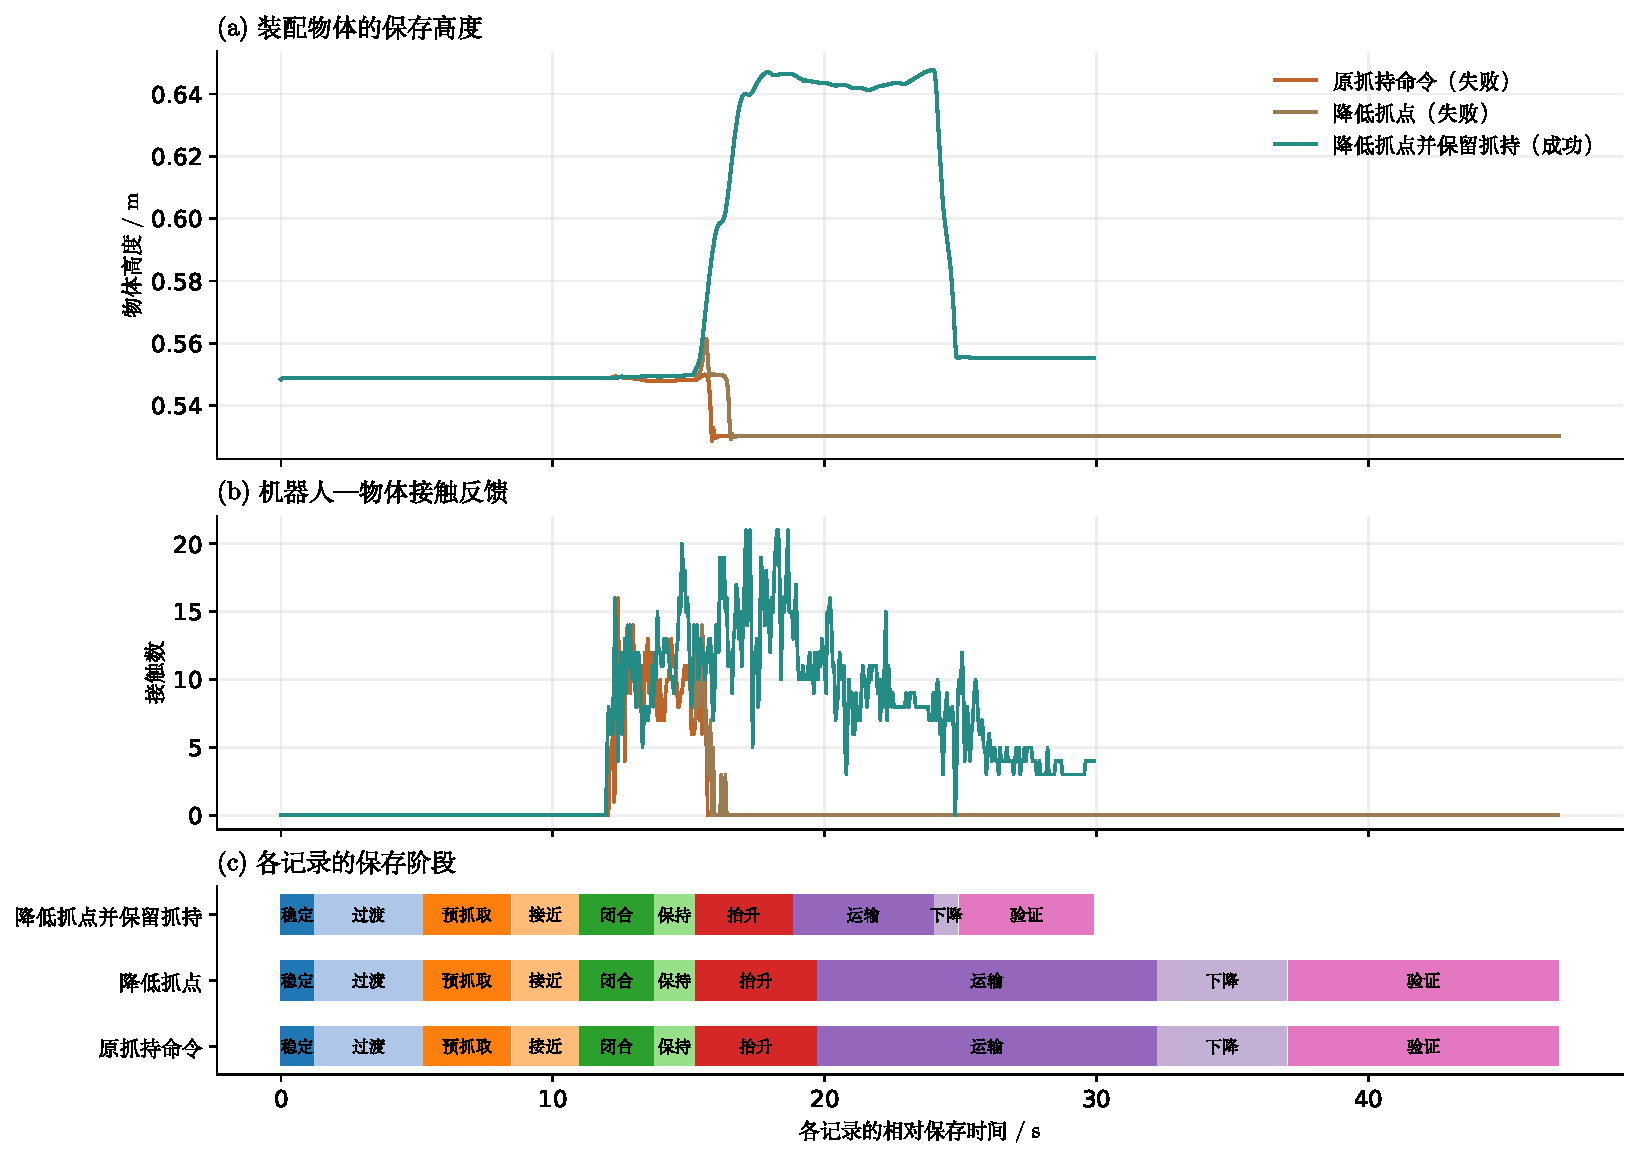
\includegraphics[width=0.97\textwidth]{figures/annotation_R2/assembly_failure_records.pdf}
\caption{装配历史成功与失败记录的物体高度、接触反馈和阶段对照}
\label{fig:ch03_examples}
\end{figure}

现有结果支持分层评价与任务专属控制的必要性，尚不支持模块间的公平优越性结论。缓存、variant和局部成功不合并为统一成功率；未定位原件的14物体与127物体批次不列入验证结果，也不用其他数量替代。

\section{本章小结}
\label{sec:grasp_demonstration_summary}

本章研究几何抓取候选到可执行专家示教的转换。候选表达限定手部控制变量，物理反馈检查抓持行为，可达性筛选与连续执行检验机器人运动条件，严格回放进一步检查轨迹质量。GraspQP官方指标被适配到六驱动手部代理，DexEvolve-style搜索与局部腕姿态扩展分别补充执行反馈和机器人可达性信息，条件性后续编辑用于处理部分尚未解决的案例。各环节在保留已有方法来源的基础上，分别处理抓持质量与机器人执行约束。

轨迹生成通过阶段目标、插值和控制器连续状态连接操作过程，Strict进一步区分任务成功与可用示教质量。已有批量记录、Sugar Box局部扰动Strict结果及典型任务对照提供了有限范围内的验证依据，但缓存记录、物体筛选域、历史版本及初态覆盖仍限制结论外推。五种任务共享记录合同，同时保留各自的接触、承载和目标评价逻辑。

执行成功的轨迹还需要转为语义明确的训练样本：策略在何时得到观测、下一步施加什么动作，以及这些记录来自哪次执行，都影响学习目标。下一章据此讨论多模态数据的组织、时序关联和质量审查。

% !TeX root = ../thesis.tex
% TH-CH04-R1: independent preview compiled; awaiting PDF review, not frozen.
\chapter{多源示教数据构建与质量控制}
\label{chap:multimodal_data}

\section{多模态数据表示与组织方式}
\label{sec:data_representation}

专家轨迹能够完成操作，并不意味着其保存结果已经适合训练\cite{mandlekar2022demonstrations}。模型需要知道某一观测对应哪个动作、哪些量可以作为输入，以及不同记录是否来自相同执行条件。因此，本章在第三章的示教生成基础上，研究状态、动作、视觉和触觉如何组织为可追溯样本，并通过版本与质量标记区分数据用途。这里的多源既包括不同任务和记录路径，也包括独立采集的真实触觉资料；不同来源不因具有相同维度就自动成为同步配对。

数据组织以Episode和Frame为基本单位。Episode表示一次执行及其来源记录，Frame表示该序列中保存的一行观测或转移。Root用于表示按具体规则划分的初态与来源组，不能直接由Episode数量或随机seed数量推导。一个源执行可以派生多个后缀、窗口或导出版本，文件数增加并不意味着独立物理条件增加。对于需要检验泛化的模型，还应根据实际来源确定分组边界，而不是先把所有Frame随机打散再划分数据。

策略可观测状态与完整仿真状态分开保存。当前39维state由受控执行器的13维actuator\_length、13维actuator\_velocity和13维上一位置命令构成，其顺序与机械臂七通道、手部六通道一致。机械臂坐标按角度表达，固定腱坐标按模型长度表达，相应速度单位也不同。该状态不是39个关节位置，不包含完整qpos中的全部自由物体状态；它具有对应真实机器人接口的设计意图，但不因此获得实机信号标定认证。

\begin{table}[htbp]
 \centering\small
 \caption{主要数据字段的维度与实际语义}
 \label{tab:ch04_fields}
 \begin{tabular}{p{0.25\textwidth}p{0.18\textwidth}p{0.43\textwidth}}
 \hline
 字段 & 组织方式 & 语义与单位边界\\
 \hline
 state & float32，$[T,39]$ & 执行器位置、速度及上一命令，非完整关节状态\\
 position\_action & float32，$[T,13]$ & 机械臂关节与手部执行器位置目标\\
 ik\_action & float32，$[T,13]$ & xyz、四元数和手部命令，非实测末端位姿\\
 sensor\_tactile & float32，$[T,712]$ & processed响应，无已认证Pa单位\\
 object\_state & float32，$[T,N,7]$ & 位置与四元数，条目可含固定实体或目标site\\
 qpos、qvel & $[T,D_q]$、$[T,D_v]$ & 完整仿真状态，维度随模型和物体变化\\
 timestamp等 & 每控制行一个时间值 & 仿真时钟及转移结束时间\\
 RGB & 独立视频或图像特征 & 需由时间及控制行索引关联\\
 \hline
 \end{tabular}
\end{table}

表\ref{tab:ch04_fields}中两种动作都为十三维，但语义不同。position\_action保存实际低层位置目标；ik\_action前七维为末端位置与四元数，后六维为手部命令。将IK目标当作关节位置不仅改变单位，还改变学习目标的含义。类似地，目标位姿不能作为实际测量的末端位姿使用，object\_state中的目标site也不应计为独立运动物体。触觉沿用第二章定义的712维processed观测，记录层不重新赋予其真实压力含义。

\begin{figure}[htbp]
 \centering
 \fbox{\begin{minipage}{0.91\textwidth}\centering
 原始执行：source NPZ $+$ Manifest\\[4pt]
 $\downarrow$ 字段、时序与来源核对\\[4pt]
 规范modalities $+$ Episode元数据 $+$ 验证记录\\[4pt]
 $\downarrow$ 按具体导出合同映射\\[4pt]
 LeRobot数值特征、图像或视频、Episode索引\\[4pt]
 真实触觉独立记录另行登记，不自动形成Real--Sim物理配对
 \end{minipage}}
 \caption{数据载体及其转换关系示意}
 \label{fig:ch04_carriers}
\end{figure}

原始NPZ保存密集数组，Manifest记录来源和配置，规范modalities提供统一字段，LeRobot则提供后续训练使用的特征与索引组织，关系见图\ref{fig:ch04_carriers}。这些载体并非互相独立的数据集，每次转换都需要保留父来源。格式版本还应与语义合同分开：LeRobot的codebase\_version不等于五任务在线记录版本。真实触觉窗口也不具备仿真Episode的全部动作和RGB字段，不能为了统一存储而假定缺失模态已经存在。

\section{示教数据采集与关联机制}
\label{sec:data_recording_alignment}

观测与动作的关联决定模型实际学习的问题。以执行前观测预测即将施加的动作，与给模型提供动作执行后的状态，虽然可以生成相同长度的数组，却具有不同的因果含义。若将当前动作与其造成的post-action结果直接配对，训练过程可能利用执行结果反推动作，而不是根据执行前状态选择控制。因此，采集程序需要明确每一行位于控制周期的哪个位置，不能仅依赖行号和时间递增判断关联正确。

设$u_i$为第$i$次施加的动作，$o_i^{-}$与$o_i^{+}$分别为执行前后观测。在线记录采用执行前输入；对于只保存执行后观测的历史序列，在物理连续、无隐藏重置的条件下，可使用前一行建立对应：
\begin{equation}
 \mathcal D_{\mathrm{online}}=\{(o_i^{-},u_i)\},\qquad
 \mathcal D_{\mathrm{shift}}=\{(o_{i-1}^{+},u_i)\}.
 \label{eq:ch04_causal_pairing}
\end{equation}
式\ref{eq:ch04_causal_pairing}不是对所有旧数据都成立的自动修复规则。若中间发生状态恢复、未保存的试探步骤或时间缺口，前一条记录未必就是当前动作的真实起点，需要结合实际执行路径检查。移位还要求源动作语义正确，不能修复把IK输入当成关节命令的问题。

在线记录适配器在物理推进之前采集仿真时钟、策略状态、触觉和对象姿态，推进结束后补充next\_timestamp与实际位置命令。它同时适配普通step和低层step\_physics路径，只将任务记录器最终接受的步骤提交到正式序列，避免把规划器内部探测过程混入示教。低层代码可能先写控制缓冲区再调用物理推进，因此提供prepare\_recorded\_control接口，在覆盖命令之前保存执行前状态。否则，state中的上一命令可能已被当前命令替换，破坏其原有定义。

\begin{figure}[htbp]
 \centering
 \fbox{\begin{minipage}{0.91\textwidth}\centering
 在线：读取$o_i^{-}$ $\rightarrow$ 施加$u_i$ $\rightarrow$ 得到$o_i^{+}$\\[5pt]
 训练配对：$o_i^{-}$ $+$ $u_i$\\[5pt]
 旧记录：保存$o_{i-1}^{+}$ $\rightarrow$ 当前动作$u_i$ $\rightarrow$ 保存$o_i^{+}$\\[5pt]
 合法连续时可配对：$o_{i-1}^{+}$ $+$ $u_i$\\[5pt]
 不直接配对当前执行后结果$o_i^{+}$与动作$u_i$
 \end{minipage}}
 \caption{执行前采集与历史执行后记录的索引关系}
 \label{fig:ch04_timing}
\end{figure}

触觉处理还具有内部时间状态。同一物理状态被多次读取时，如果每次都推进低通滤波或重新采样噪声，新增观测操作本身就可能改变保存值。当前适配器以仿真时间和原始读数内容作为缓存键，同一键只处理一次并返回副本，使额外采集不重复推动信号处理。该机制解释了为什么记录层不仅需要调用传感器接口，还需管理读取时机；它是当前代码的行为，不能回填为所有历史记录均具有的属性。

状态、动作和触觉按控制周期保存。$t_i$对应第$i$条被接受记录在执行前采集的timestamp，$t_i^{+}$对应该控制步推进结束后保存的next\_timestamp；$t_{i+1}$则是下一条被接受记录的执行前时刻。当前在线合同检查
\begin{equation}
 t_{i+1}-t_i\simeq\Delta t_c,\qquad
 t_i^{+}-t_i\simeq\Delta t_c,\qquad \Delta t_c=0.05~\mathrm{s},
 \label{eq:ch04_time_interval}
\end{equation}
其中近似相等表示按实现容差比较浮点时间。仅在相邻控制步连续执行且均被记录、期间没有额外物理推进或重置时，$t_{i+1}$才与$t_i^{+}$一致。未接受步骤、跳步或异常中断可能使两者不再衔接，不能将此关系推广到存在记录缺口的序列；在线检查会拒绝不满足连续时间合同的数据。视频PTS可使用相对帧时间，仿真时间则保留绝对时钟，两者需要由首帧偏移和采样索引连接。时间单调只能排除部分结构错误，不能证明每张图像确实来自对应物理状态。

\begin{figure}[htbp]
 \centering
 \fbox{\begin{minipage}{0.91\textwidth}\centering
 20~Hz控制行：0，1，2，3，4，5，6，7，8，$\ldots$\\[5pt]
 状态与触觉：每个被接受的控制行记录\\[5pt]
 默认20~Hz RGB：0，1，2，3，4，5，6，7，8，$\ldots$\\[5pt]
 5~Hz RGB示例：0，4，8，$\ldots$；保留对应控制行索引\\[5pt]
 图像降频不删除中间控制行，不填造缺少的图像
 \end{minipage}}
 \caption{控制记录与RGB采样频率分离的合同示意}
 \label{fig:ch04_multirate}
\end{figure}

RGB具有独立采样配置。默认合同为1920$\times$1080、20~Hz，速度配置可降至640$\times$360、5~Hz，状态和控制仍为20~Hz。图\ref{fig:ch04_multirate}说明，低频图像需要保存其控制行索引，而不是删除两张图像之间的动作。程序按显式合同检查采样位置，不能把默认视频频率当作全部服务器数据的实测参数。

\begin{table}[htbp]
 \centering\small
 \caption{不同记录路径的时序与版本边界}
 \label{tab:ch04_recording_versions}
 \begin{tabular}{p{0.21\textwidth}p{0.34\textwidth}p{0.31\textwidth}}
 \hline
 路径 & 关联方式 & 使用限制\\
 \hline
 旧生成记录 & 执行后观测及动作列 & 须核对动作语义和索引偏移\\
 修复版LeRobot导出 & 可执行ctrl与前一源观测 & 仅对实际重导出且核验的数据成立\\
 在线记录 & 执行前采集、执行后补实际控制 & 需检查预备控制与接受步骤是否对应\\
 v4精确辅助合同 & 增加完整积分状态和float64控制 & 支持回放，不替代观测关联审查\\
 \hline
 \end{tabular}
\end{table}

Episode终止与异常中断同样影响可保存范围。在线适配器只有在完成对应物理步骤并被记录器接受后才提交行，视频编码异常需向上层传播，不能继续登记缺失模态。表\ref{tab:ch04_recording_versions}中的版本区别因此不仅是字段增减，还涉及生成顺序和验证范围。修复代码的存在、数据已重新导出以及数据通过重新审计是三个不同状态，旧文件不能仅因程序更新而自动获得新合同标记。

\section{数据格式转换与统一存储}
\label{sec:data_conversion}

统一存储的目标是使不同执行来源具有可识别的字段和验证信息，而不是把所有十三维数组都重命名为action。规范数据包从源position\_action映射训练action，从sensor\_tactile映射训练tactile，保留执行前state、时间与对象信息。源NPZ和Manifest仍随包保存，使转换结果可以回到原记录检查。LeRobot导出则进一步按其特征定义组织数值和图像数据；已经存在规范NPZ包，并不意味着对应LeRobot版本也已生成。

历史导出修复首先处理动作来源。Strict回放所需低层控制来自ctrl，而非旧记录中的笛卡尔action。导出器检查控制序列与源ctrl的尾部对应关系，再选取前一条执行后观测作为相应执行前输入。重新执行导出时，程序直接在step之前读状态和图像，之后才施加动作；非重新执行路径则恢复源观测所在的仿真状态，并使用对应触觉。两条路径需要分别记录，不将恢复后渲染与新物理执行混称。

P31时序修复对等长数组执行观测截去末行、动作截去首行的操作，并保存偏移说明和被丢弃的首动作索引。它改变了配对关系，但不自动把IK动作变为关节命令。因此，动作语义修复和索引修复必须独立检查；仅通过shape、finite或调用名为causal的函数，均不能说明训练目标已经正确。对于字段不完整或来源不明的文件，应保留旧版本身份，而不是补零后强行进入统一格式。

转换一致性以同一字段和同一索引下的数值差评价。设源字段按映射$\pi$取值，转换后字段为$\hat{\boldsymbol x}_i$，使用
\begin{equation}
 E_{\max}=\max_{i,j}\left|\hat{x}_{i,j}-x_{\pi(i),j}\right|
 \label{eq:ch04_mapping_error}
\end{equation}
检查指定映射。误差为零只对所比较字段成立，不能扩大为未检查图像、完整状态或物理回放一致。若变换包含量化或重采样，还需按实际合同设置误差解释，而不能一律要求任意格式变换逐比特相同。

指定Sugar Box源共有477行，修复版LeRobot导出340行。按零基索引，导出动作对应源ctrl第137至476行，状态命令和触觉对应前一源行，即第136至475行。本次材料核验重新比较这340行，动作、state末十三维命令以及对应源tactile的最大绝对差均为0。该结果为单一明确来源提供了可复核映射，不代表全部39维状态、RGB像素或其他导出目录均已认证。

v4规范包还保存float64完整积分状态及实际控制，供后续回放使用，这些辅助字段与策略输入分开。Manifest与Episode元数据记录源文件、转换合同及SHA256，文件Hash用于确认文件是否改变，来源说明用于解释其语义。两者缺一不可：相同字段名称或相同文件Hash并不能替代采集与索引规则，统一存储需要的是可追溯合同，而不是只有统一目录形式。

\section{轨迹质量审计与数据清洗}
\label{sec:data_quality_control}

数据质量不能由单一成功标签决定。任务执行成功说明机器人在给定条件下完成目标，Strict通过说明对应轨迹满足特定稳定性约束；两者均未直接检查训练动作的含义或观测时序。反过来，数组finite、shape合法也不说明轨迹完成任务。因此，本章将质量控制分为执行与验证状态、结构数值、时间关联、来源版本、重复隔离以及训练角色六个层次，使每一层回答明确的问题，而不将全部检查折叠成一个模糊的有效标记。

\begin{table}[htbp]
 \centering\small
 \caption{分层数据质量检查及其判定范围}
 \label{tab:ch04_quality_gates}
 \begin{tabular}{p{0.18\textwidth}p{0.36\textwidth}p{0.32\textwidth}}
 \hline
 层次 & 检查对象 & 不能单独推出的结论\\
 \hline
 执行与验证 & 任务结果、Strict配置及状态 & 不证明动作导出和关联正确\\
 结构与数值 & shape、dtype、finite、触觉非负 & 不证明物理合理或任务成功\\
 时间与动作 & 时间间隔、上一命令、物理状态连续 & 不认证全部视频像素同步\\
 来源与版本 & Manifest、源Hash、模型和合同 & 不自动证明跨版本物理等价\\
 重复与隔离 & lineage、content及队列状态 & 不保证独立Root或无近似重复\\
 训练角色 & 标签、组划分及来源用途 & 不由格式合法自动获得训练准入\\
 \hline
 \end{tabular}
\end{table}

结构检查约束state、position\_action、ik\_action和sensor\_tactile的形状与float32类型，检查对象姿态、数值有限性、触觉非负及时间增量。对于已声明版本的阶段编码，还需保证阶段数组长度一致、编码不重复且观测到的编码具有合法含义。字段缺失不能默认为零，尤其不能把未记录触觉伪装成全零触觉。时间和命令连续性检查则需要相应字段及开关实际启用，不能从函数返回的版本名称直接推断所有检查都已执行。

在线状态中的上一命令可以与前一行实际动作比较，保存的执行前qpos/qvel也可与上一行执行后状态比较。这些关系可检出部分记录错位或隐藏状态跳变，但不能替代完整物理回放。旧PickPlace案例中，state后十三维与前一position\_action比较，有373个相邻转移超过$10^{-6}$容差，最大差约0.1。这一发现说明该记录不满足当前命令连续性检查，并不能在没有进一步定位时断言其全部模态反因果或指定唯一故障原因。

旧Stack案例则没有pre\_qpos和pre\_qvel，无法完成当前要求的物理连续性核验。它与旧PickPlace还缺少规范modalities文件，不能描述为所有旧记录都已经完成统一导出。这里的处理是保留问题和版本身份，而不是在本轮删除、补写或重建数据。审计发现的缺陷应与影响范围一起保存，否则后续程序可能仅因旧文件能够读取就重新把它当作已修复数据。

\begin{figure}[htbp]
 \centering
 \fbox{\begin{minipage}{0.91\textwidth}\centering
 执行结果与验证状态 $\rightarrow$ 结构、数值及阶段合同\\[4pt]
 $\downarrow$\\[4pt]
 时间关联与动作语义 $\rightarrow$ 来源、版本与文件Hash\\[4pt]
 $\downarrow$\\[4pt]
 内容重复与用途检查 $\rightarrow$ VALIDATING后登记\\[4pt]
 $\downarrow$\\[4pt]
 登记：\mbox{EXPORTED} / \mbox{DUPLICATE}；异常隔离：\mbox{QUARANTINED}\\[4pt]
 训练准入仍需对应标签、分组与研究用途
 \end{minipage}}
 \caption{分层质量审查与数据准入关系}
 \label{fig:ch04_admission}
\end{figure}

来源检查将规范数组与原始在线记录逐项对应，并核对登记文件Hash、源Manifest、模型证明及独立回放记录之间的绑定。完整积分状态和float64控制可以提供更充分的回放起点与命令，但辅助数组存在并不意味着实际回放已经使用它们，仍需相应证明。图\ref{fig:ch04_admission}中的各层因而既检查数据，也检查执行了哪些验证；代码具有某项能力和某个数据包通过该项验证需要分开记录。

队列通过任务状态、租约和事务组织提交。worker在有效lease下提交结果，登记要求进入\mbox{VALIDATING}且外部verification明确通过。登记时，来源或内容重复者进入\mbox{DUPLICATE}，无重复者插入Episode表并进入\mbox{EXPORTED}；\mbox{QUARANTINED}属于失败或重试耗尽后的隔离路径，并非成功登记的另一出口。过期租约、重试上限和隔离机制用于处理异常，不能让旧worker继续登记已失去所有权的任务。文件写入、验证与数据库登记是不同步骤，异常恢复需要对照已有文件和状态，而不能仅依据进程是否存在判断数据已完整保存。上述机制是实现事实，不代表任意磁盘断连之后都已经证明无损恢复。

重复检测同时使用来源和内容标识。对于待登记记录$e$及已登记集合$\mathcal A$，当前逻辑可表示为
\begin{equation}
 \operatorname{dup}(e)=\boldsymbol 1\!\left[
 \exists e'\in\mathcal A:\ L(e)=L(e')\ \lor\ C(e)=C(e')\right],
 \label{eq:ch04_duplicate}
\end{equation}
其中，$L$与$C$分别为lineage和content标识。相同来源或相同语义内容任一成立，即进入重复处理，而不是要求两个Hash同时相同。lineage绑定任务、资产与源文件，content则根据规范数组和解码RGB摘要生成；时间使用相对首行的表示，精确回放辅助字段不参与内容摘要，以减少仅改变时钟或多存辅助信息造成的重复计账。

Hash只能识别定义范围内的相等，不能证明两个不同Hash具有不同物理初态，也不能排除近似轨迹或相同模板派生的样本。训练划分还需要按来源组管理，同一Root的窗口、后缀和重导出版本不能因文件不同而分散到训练与验证两侧。对于缺少完整lineage的历史文件，应把独立性标记为未知，而不是用新的随机划分掩盖来源缺口。

数据清洗也不应等同于删除所有失败轨迹。合法失败仍可用于失败诊断或具有明确标签的其他研究，但不能直接当作成功专家标签；是否计入生产时长应遵循对应冻结规则。历史版本保留来源和合同标记，既能支持修复效果比较，也能避免旧性能结论继续建立在错误语义上。表\ref{tab:ch04_quality_gates}所示分层审查因此强调按用途准入：任务成功、Strict通过、格式有效、时序正确与可用于具体训练之间存在依赖，却不能互相替代。

\section{数据集统计与质量验证}
\label{sec:dataset_quality_validation}

本节以明确的数据范围检验上述合同和审查机制。材料核验直接读取三组LeRobot目录的全部选定数值Parquet行，以及十一条指定源NPZ，后者包括五条旧在线记录、五个v4开发包和一个Sink精度对照源。数字均绑定对应目录与版本，不以历史summary替代当前读取结果。对于视频解码、物理回放或真实触觉原始全库，本轮没有重新执行相应验证，其已有合同和成绩分别标明来源层级。

三组LeRobot库存见表\ref{tab:ch04_lerobot_inventory}。实际episode\_index数量和Parquet行数与info中的Episode、Frame声明一致，state、action和tactile分别符合39、13、712维，所读数值finite，触觉非负。这个结果说明指定数值文件可按所声明结构读取，但不证明早期版本的动作语义和时序正确。两个旧目录仍保留其历史合同问题，不能因为当前程序已经修复，就把旧数据和模型性能重新解释为合规基线。

\begin{table}[htbp]
 \centering\small
 \caption{三组LeRobot数据的实际数值库存}
 \label{tab:ch04_lerobot_inventory}
 \begin{tabular}{p{0.30\textwidth}rrp{0.27\textwidth}}
 \hline
 数据版本 & Episode & Frame & 使用范围\\
 \hline
 早期五条导出 & 5 & 1550 & 历史格式及合同问题对照\\
 早期formal30导出 & 30 & 14310 & 保留原版本，不自动认证语义\\
 Sugar单物体修复版 & 1 & 340 & 指定源数值映射核验\\
 \hline
 \end{tabular}
\end{table}

三组数据的触觉非零比例分别约为12.7297\%、9.4029\%和11.0972\%，这是对各目录所选全部数值行的重新计算，不是任务成功率或物理准确率。task\_index分别对应两个、三个和一个lift:物体标签，实际都属于Lift操作，不能解释为覆盖两种、三种和一种物理任务。三个info均仅声明train范围，未提供本轮可认证的独立验证和测试划分。Episode数量因此不能直接替代独立Root数量，也不能将三个版本相加为36个独立采集主体。

修复版的一致性检查进一步回到原始来源。340行导出action与源ctrl、state命令区与前一源ctrl、触觉与前一源tactile均得到最大绝对差0，支持该索引映射在指定数值字段上成立。它不意味着所有39维状态都已单独重算，也不包括RGB像素逐帧检查。对三组数据的完整Episode数值摘要比较未发现完全相同的摘要，但这一检查既不含图像，也不排除截断后缀、轻微差异或同源版本重复，不能据此宣布无泄漏。

\begin{table}[htbp]
 \centering\small
 \caption{旧在线记录与v4开发包的质量对照}
 \label{tab:ch04_version_quality}
 \begin{tabular}{p{0.23\textwidth}p{0.34\textwidth}p{0.29\textwidth}}
 \hline
 对象 & 本次材料核验结果 & 限制\\
 \hline
 旧PickPlace & 373个转移命令关系超容差，最大约0.1 & 不满足当前连续性检查，未修复\\
 旧Stack & 缺pre\_qpos、pre\_qvel及modalities & 物理连续性UNKNOWN\\
 五任务v4开发包 & 2727行，字段映射及登记文件Hash匹配 & 开发准入，非正式生产验收\\
 v4独立性标识 & 5个lineage、4个asset\_hash、5个content值 & 不等于认证独立Root数\\
 \hline
 \end{tabular}
\end{table}

旧五任务在线样本共2665行，表\ref{tab:ch04_version_quality}中的PickPlace与Stack缺陷说明，同一历史批次也不能只依据某个样本通过就整体升级。相对地，所选五个v4包覆盖Lift、PickPlace、Stack、Push和NutAssembly，共2727个控制行。其命令及所存qpos/qvel连续性检查通过，规范action、触觉、state与源映射逐项一致，登记文件Hash全部匹配且无登记文件缺失。这里确认的是保存数据及文件关系，不能替代新的物理执行。

五个v4包有五个lineage、四个登记asset\_hash及五个登记content值，独立Root数仍为UNKNOWN。包中admission明确为开发验证，而非正式生产准入。五个视频文件都存在，只能作为文件覆盖证据；本轮没有对全部RGB解码及逐帧同步重新认证，也没有独立重算包含解码视频摘要的语义content hash。历史视频验证记录可以随版本引用，却不应升级为本轮完成的视频验收。

历史Sink对照提供了回放合同影响的另一实例。同一380帧源在旧float32路径下回放失败，最大qpos分量偏差为1.628897；保存完整积分状态并使用float64控制的路径回放通过，记录偏差为0，见表\ref{tab:ch04_sink_precision}及图\ref{fig:ch04_sink_precision}。这些数值来自已保存回放报告，不是本轮新实验；本轮只读取源数组并确认辅助字段和数据类型。qpos包含不同类型的坐标，最大分量偏差也不能统一解释为某一长度误差。

\begin{table}[htbp]
 \centering\small
 \caption{Sink历史回放状态与精度对照}
 \label{tab:ch04_sink_precision}
 \begin{tabular}{p{0.46\textwidth}rp{0.17\textwidth}}
 \hline
 历史回放路径 & 最大qpos分量偏差 & 历史结果\\
 \hline
 旧float32状态及控制路径 & 1.628897 & 失败\\
 完整积分状态与float64控制路径 & 0 & 通过\\
 \hline
 \end{tabular}
\end{table}

\begin{figure}[!htbp]
 \centering
 \setlength{\abovecaptionskip}{0pt}
 \vspace{-10pt}
 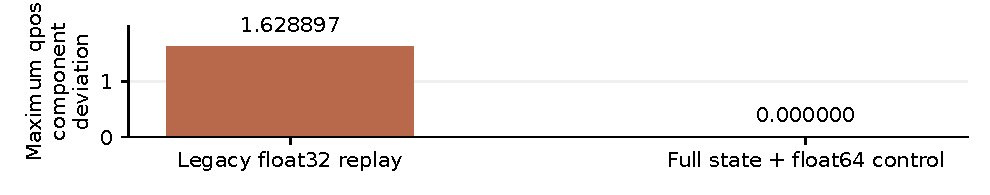
\includegraphics[width=0.78\textwidth]{figures/ch04/sink_historical_precision_r2.pdf}
 \caption{由已有报告绘制的Sink回放偏差对照（历史记录，非本轮新实验）}
 \label{fig:ch04_sink_precision}
 \vspace{-14pt}
\end{figure}

两种设置同时改变完整状态保存与控制精度，因此该对照支持原状态/精度合同不足的解释，但没有分离两个因素的独立贡献。偏差0也只指报告中对应保存状态的比较方式，不能推广为任意任务、模型版本和浮点后端均逐位复现。保存额外状态能够增加回放证据，却不产生新的物理多样性；同一条件的旧隔离副本和新通过副本不能重复累计为新增时长。

真实触觉与Natural Sim的冻结训练合同需另行登记，不混入上述Episode与Frame库存。已有P44合同声明Real Train为5153窗口、32 Session，Real Validation为780窗口、4 Session；Natural Train为4049窗口、50 Root，Validation为905窗口、10 Root。这些是历史合同声明，本轮未重新认证原始Real全库。合同还保留Real历史不等间隔帧与Natural来源20~Hz连续采样的区别，因此不能把四帧窗口数量解释为同样的物理持续时间或相同数量的独立接触过程。

Real记录与仿真示教没有已认证同步物理配对，物理通道映射也仍有限制。它们可以按来源组织，并用于后续明确监督条件的跨域研究，但不能作为已经同步的视觉、动作与真实触觉联合数据集。Validation名称本身也不消除历史开发暴露，训练角色和独立性需要结合实际使用记录解释，而不是仅凭文件名判断。

本节统计不覆盖服务器批次2的实时数据库和完整磁盘。当前全量有效小时、独立Root及全局泄漏状况均不能由这几组样本外推。重复读取扩容索引反映的是采样使用量，不是新增物理仿真时长。现有证据支持版本化合同能够发现问题、指定转换和开发包满足所列检查；它尚不支持全部历史数据均可训练、全任务模态完全同步或正式生产指标已通过的结论。

\section{本章小结}
\label{sec:data_quality_summary}

本章从训练样本需要具有明确输入、动作和来源关系出发，建立了多模态数据表示、采集关联、规范转换及分层审查的论证。39维策略状态与完整仿真状态分开，两种十三维动作按语义区分，触觉和RGB按各自采样合同关联。执行前记录、控制缓冲预备和触觉缓存共同说明，采集时机本身是数据定义的一部分，不能由格式和维数代替。

已有数据核验确认了指定Sugar导出字段与源记录的一致性，也发现旧PickPlace命令连续性和旧Stack字段缺失问题。五任务v4开发包及Sink历史回放对照提供了版本化质量控制的有限依据，但不构成服务器全量验收、独立Root认证或全局无泄漏证明。保留来源、Hash、验证层级和失败记录，使这些局限能够被明确识别，而非通过统一文件名掩盖。

在上述数据条件下，后续研究需要进一步区分真实触觉与仿真触觉的分布及监督关系。下一章将基于已保存的真实统计信息和冻结触觉子集讨论跨域重建，不将规范化存储等同于两域已经具有同步物理对应。

% !TeX root = ../thesis.tex
% CH05-FINAL 2026-11-21. Authoritative sources mapped in integration manifest.
\chapter{基于统计伪配对与双域表示的触觉跨域重建方法}
\label{chap:dual_domain_reconstruction}

% Active section fragment; included through body/ch05_dual_domain_reconstruction.tex.
\section{真实与仿真触觉差异分析}
\label{sec:ch05_real_sim_difference}

真实与仿真触觉具有相同数组维度，并不意味着能够直接用于同一操作表示。本文采用的观测按16个Patch组织，共712个标量通道，仿真阵列覆盖五指及手掌。其传感器原生raw读数来自MuJoCo native touch，对感知区域内的法向接触力累加\cite{mujoco2026xml}；仿真processed观测则经过死区、限幅、非线性响应、时间滤波及Patch内邻域扩散处理（实现参数名为crosstalk）。Real processed观测来自实机自身采集处理流程，因此两域processed均应视为处理后的数值响应，不能直接称为真实压力或共同力学单位。对这种观测进行迁移，需要检查保留了哪些接触信息，而不只是核对输出形状。

P37旧开发数据的Real Train/Validation为5153/1408窗，Sim为1824/406窗；P43当前主线中，Real Train/Validation分别为5153/780窗，Natural Sim Train/Validation分别为4049/905窗，均采用$4\times712$窗口。P37统计不外推至P43，后者规模仅描述当前数据划分，不代表差异复现。后续统计按相应版本分别报告，并以来源分组考察样本独立性。

令$X_{tj}$为第$t$帧第$j$通道响应，精确非零Mask定义为$M_{tj}=\mathbf1[X_{tj}>0]$。在旧训练集上，Real与未转换Sim的激活比例分别约17.60\%和13.31\%，说明数值支持范围存在差异。Mask表示保留每帧712个激活位置，可以反映Patch内部支持及区域组合，却不是物理接触真值。滤波残留等微弱正值也会计入激活。因此，Mask首先反映数值支持范围；跨域热图按固定通道索引比较，物理配准的前提在下一节统一界定。

幅值分析仅取$X>0$的响应。旧训练集汇总正值中位数，Real约为0.00500250，未转换Sim约为$1.03974\times10^{-5}$；P95分别约1.50101与0.459485。这些是各域全部正值池的统计，不是逐Patch分位数的平均，也不是接触力误差。幅值分解以每帧正值的P10、P25、P50、P75、P90构成有效$4\times5$表示，其余通道仅补零以复用网络接口；不输入Taxel位置、正值数量或空Patch标志。对包含至少一帧全零响应帧的窗口，按照预定规则予以排除，故该表示只刻画有响应条件下的幅值，不能覆盖完全无接触状态。

表\ref{tab:ch05_domain_feature_difference}列出旧P37数据上既有转换输出经幅值校准后的表示分解诊断。Full与分位数先作log1p，各表示分别用Train拟合标准化，Probe由Logistic、kNN各1个及MLP、GRU、Transformer各Seed11、12、13组成，共11个；Full复用P38在相同输出、划分和预处理上的Probe拟合，不新增训练。此处为迁移后Probe诊断，非后文迁移前冻结的域分类评价基线（C0）验收。定义$D=1-2|\mathrm{BA}-0.5|$，只度量BA偏离0.5的程度；表中三个表示的最小D均低于0.90，表明至少存在Probe未满足固定阈值下的BA等价门槛；其排序判别能力仍需结合AUC判断。因此，不能仅凭这些结果认定支持或正值摘要已经实现域混淆。幅值调整保持Mask不变，不代表完整触觉已匹配。

\begin{table}[htbp]
 \centering\small
 \caption{旧P37数据校准后触觉的表示分解诊断}
 \label{tab:ch05_domain_feature_difference}
 \begin{tabular}{llc}
 \hline
 表示&有效内容&11个Probe实例中的最小D\\\hline
 Mask&$4\times712$精确非零支持&0.0272\\
 Amplitude&$4\times5$正值分位数&0.1494\\
 Full&$4\times712$完整响应&0.0573\\\hline
 \end{tabular}
\end{table}

三种表示的特征空间、预处理及纳入条件不同，D值不能相减计算信息贡献，也不证明支持与幅度独立。低维分位数舍弃了响应所在通道及跨Patch组合，即使边际分布相似，也可能无法维持原接触结构。差异还可能来自任务构成、采集协议与处理链，不能全部归因于传感器物理性能。

四帧窗口还承载激活持续、出现、消失及幅值变化。P37验证集第1至第2帧的Mask变化比例，Real约1.7154\%，未转换Sim约0.0958\%，分母为各自窗口与通道总数，而非条件转移概率。真实帧间隔并非恒定，帧间差分不能直接解释为物理时间导数或频率差异。幅值还需检查相邻帧全通道绝对差，不能仅用Mask持续性代替响应强度变化。因此，完整重建应同时保留激活支持、正值幅度及短时序关系。下一节据此在缺少同步物理配对的条件下定义跨域重建问题。

% Active section fragment; included through body/ch05_dual_domain_reconstruction.tex.
\section{非配对条件下的跨域触觉重建问题定义}
\label{sec:ch05_unpaired_problem}

前节表明，真实与仿真触觉即使具有相同观测维度，其激活支持、幅值及短时序关系也不能直接互换。本文以自然任务仿真产生的processed触觉为输入，研究向Real域风格观测的转换。单个窗口包含四帧、每帧712个通道，输入与输出均保留既有通道及帧序。目标输出应为完整$4\times712$的有限非负数值，保留精确零值与非零激活支持，并具有Real域processed统计特征，不将其直接称为真实传感器输出，也不以低维统计摘要代替完整观测。保留帧序不要求两域采样间隔相同，帧间变化也不直接表示物理时间导数。

本章使用第\ref{sec:data_quality_summary}节所区分的单独登记并冻结的触觉子集，不直接读取LeRobot示教导出。其中三类数据分别承担不同角色：Real提供真实域观测，用于域内表示学习，并提供统计先验及伪配对目标侧信息；Natural Sim来自自然任务仿真，与Paired Sim共同参与Sim域表示学习，也是最终转换对象；Paired Sim则由真实统计先验指导仿真物理探针生成，按登记关系与Real窗口构成统计伪配对，为潜变量映射提供有限监督。任意Real与Sim窗口并无已知共同接触状态，不能直接互作真实标签。现有1200个训练窗口与240个验证窗口也不代表1440个独立Root；登记关联不构成同步物理接触真值，来源复用与覆盖限制仍须保留。Natural参与Sim表示学习，不等于其具有对应Real目标，亦不等于直接参与原始配对映射训练。

记Natural Sim窗口为$X_S$，Real域风格输出为$\widehat X_R$，待学习映射为$F_\theta$，问题定义为
\begin{equation}
 \widehat X_R=F_\theta(X_S),\qquad
 F_\theta:\mathbb R_{\geq0}^{4\times712}
 \rightarrow\mathbb R_{\geq0}^{4\times712}.
 \label{eq:ch05_unpaired_mapping}
\end{equation}
目标同时包括接近Real完整观测统计，以及尽可能保留源输入的空间索引结构、激活支持、幅值和短时序变化；后者是待检验要求，不是已实现的物理语义保持。两域Taxel尚无逐一物理对应认证，也未建立共同力学单位；同维潜表示不意味着共同语义坐标。现有监督不提供Natural输入的同步Real真值，因而潜变量回归误差及真实Mask条件下的Decoder似然，均不能代替自由输出质量。上述目标不等同于模型实际优化的联合损失，真实机器人任务收益也尚未得到验证。

据此采用三层分析框架：输出层检查完整$4\times712$、数值有效性、激活支持、正值幅值和短时序关系，形状正确不足以认定结构保持；这些结构维度不另设未经验证的统一通过阈值。域评价沿用原始Real Train 5153窗与Natural Sim Train 4049窗训练后冻结的11个C0实例，即Logistic、kNN各一个及MLP、GRU、Transformer各Seed11、12、13，保留模型权重、kNN参照库、原Scaler与log1p、通道及帧序、Real=1与Sim=0标签、0.5阈值和原Train/Validation/Test分组，迁移评价不重训分类器或重拟合Scaler。BA取两类召回率的均值。每个实例须同时满足BA在$[0.45,0.55]$、AUC在$[0.475,0.525]$以及
\begin{equation}
 D=1-2|\mathrm{BA}-0.5|\geq0.90,
 \label{eq:ch05_domain_confusion_target}
\end{equation}
且11个实例全部满足才完成联合验收。BA与D门槛数学等价，不是两项独立证据，AUC另行评价分数排序；该检验只覆盖既定判别器，不能证明全部域信息消失。评价使用780个Real与905个Translated Natural Sim开发Validation窗口，不包装为独立盲测。物理与任务层仍需物理对应关系、同步接触真值或真实机器人操作等独立证据进一步验证，目前尚未获得充分认证。三层用于组织分析，并非已经全部通过；当前完整迁移目标仍未完成，后续分别展开监督构建、表示与映射，并检验其有效范围。

% CH05-5.3 only: standalone section fragment, not included in thesis.tex.
\section{GMM统计先验引导的仿真触觉伪配对构建}
\label{sec:ch05_gmm_pseudopairs}

真实与仿真触觉存在统计差异，而当前数据缺少经过认证的同步物理接触配对，不能将任意两条序列直接作为对应真值。真实数据中仍包含响应聚集位置、扩散范围及多峰结构等信息。为利用这些信息，本文以真实训练数据建立高斯混合模型（Gaussian Mixture Model，GMM）统计先验，引导球形探针在仿真手部形成接触，再通过原有传感器链路获得触觉输出。图\ref{fig:ch05_gmm_physical_pipeline}给出构建过程。所得配对提供统计监督，不代表两域经历了相同的物理接触。

\begin{figure}[htbp]
 \centering
 \fbox{\begin{minipage}{0.91\textwidth}\centering
 Real Train $\rightarrow$ Patch索引偏移统计 $\rightarrow$ 冻结GMM\\[2pt]
 $\downarrow$ 对指定Real目标作分量响应分解\\[2pt]
 字典位置检索与加载估计 $\rightarrow$ 球形探针物理执行\\[2pt]
 $\downarrow$ 原生触觉读取与既有信号处理\\[2pt]
 完整$4\times712$响应 $\rightarrow$ 统计准入与伪配对登记
 \par\vspace*{2.5mm}
 \end{minipage}}
 \caption{GMM统计先验引导仿真接触与伪配对构建流程}
 \label{fig:ch05_gmm_physical_pipeline}
\end{figure}

GMM按Patch建模。各Taxel行列索引映射至$[-0.5,0.5]^2$网格，以训练集该Patch正值响应的第5百分位筛选有效响应。每个Session最多取48帧，每帧按响应权重抽取16个位置，并减去该帧响应质心；随后按Session轮转抽样，形成最多2048个二维偏移点。因此，拟合对象是响应相对质心的扩散偏移，而非原始712维数组、物理压力或后续VAE潜变量。记偏移为$\boldsymbol u$，第$p$个Patch的分布为
\begin{equation}
 p_p(\boldsymbol u)=\sum_{k=1}^{K_p}\pi_{pk}
 \mathcal N(\boldsymbol u;\boldsymbol\mu_{pk},\boldsymbol\Sigma_{pk}),
 \qquad \sum_{k=1}^{K_p}\pi_{pk}=1.
 \label{eq:ch05_gmm_prior}
\end{equation}
其中，$\pi_{pk}$为混合权重，$\boldsymbol\mu_{pk}$和完整协方差$\boldsymbol\Sigma_{pk}$描述偏移中心与扩散。实现采用EM拟合，候选分量数为1、2、3，最多60次迭代，以BIC选择，并检查Session三折核稳定性。协方差初始化与更新分别加入$0.0025\boldsymbol I$和$0.0004\boldsymbol I$正则项。虽保存了分阶段模型，本节逆构造使用全阶段合并先验；参数拟合不使用Real Validation。BIC采用$-2\log L+(6K_p-1)\log n$，其中$n$为拟合偏移点数，不能作为独立采集数量。若阶段数据不足，回退同Patch合并阶段数据；三折平均核总变差超过0.25且\mbox{分量数}大于1时，回退单分量模型。对Session限制取帧并轮转抽样，可减轻长记录对拟合样本构成的支配，但不消除会话间差异。

对指定Real窗口，令$w_{pj}$为Taxel四帧平均响应，$\boldsymbol q_{pj}$为固定网格坐标。当前实现直接在该网格评估冻结分量，计算责任度及分量响应量：
\begin{equation}
 \begin{aligned}
 r_{pjk}&=\frac{\pi_{pk}\mathcal N(\boldsymbol q_{pj};\boldsymbol\mu_{pk},\boldsymbol\Sigma_{pk})}
 {\sum_{\ell=1}^{K_p}\pi_{p\ell}\mathcal N(\boldsymbol q_{pj};\boldsymbol\mu_{p\ell},\boldsymbol\Sigma_{p\ell})},\\
 m_{pk}&=\sum_j w_{pj}r_{pjk},\qquad
 \boldsymbol c_{pk}=\frac{\sum_j w_{pj}r_{pjk}\boldsymbol q_{pj}}{m_{pk}}.
 \end{aligned}
 \label{eq:ch05_gmm_responsibility}
\end{equation}
仅处理$m_{pk}>0$的分量。软责任度分解Taxel响应，并非物理接触归属概率；$\boldsymbol c_{pk}$由原网格重加权获得，并非分量均值加回目标质心。训练坐标已中心化，逆构造却未减去目标质心，二者存在原点语义不一致。故仅能作启发式权重，不保证空间先验的平移一致性。

\begin{table}[htbp]
 \centering\small
 \caption{球形探针响应字典的组织}
 \label{tab:ch05_probe_dictionary}
 \begin{tabular}{p{0.28\textwidth}p{0.59\textwidth}}
 \hline
 条件或字段 & 实际设置与含义\\
 \hline
 接触区域与位置 & 16个Patch，各取中心及上下左右共5个位置\\
 探针与加载 & 半径4~mm；基础深度0.25、0.5、1~mm\\
 手部初态设置 & 2种驱动指令；与位置、深度组合成480行\\
 记录及取窗 & 每条32帧，固定取零基索引12--15帧\\
 状态指纹 & 首个保存步的qpos与目标球心量化后联合散列，共160种，非独立Root认证\\
 响应与来源 & 原生及processed触觉、探针条件和Episode来源\\
 \hline
 \end{tabular}
\end{table}

字典将可执行条件与观测响应关联，见表\ref{tab:ch05_probe_dictionary}。各Patch分量按$m_{pk}$合并排序后保留最多5个。对每个保留分量，先在手部驱动指令为0、深度0.25~mm且非零响应的字典条目中，选择响应质心最接近$\boldsymbol c_{pk}$的位置；再利用同位置的响应总量与深度关系插值估计基础加载。四帧Patch总量相对其均值的变化用于设置加载因子，而不直接写入触觉数组。基础命令受既定范围约束，不能解释为真实材料压陷量。具体而言，四帧加载因子限制在$[0,2]$；反馈按目标与生成Patch总响应之比估计调整倍率，并将倍率限制在$[0.5,2]$、基础深度限制在$[0.1,1]$~mm。该估计依赖两域processed响应的数值关系，未建立共同力学量纲，因此触及控制边界不能被解释为已经达到正确接触强度。

\begin{figure}[htbp]
 \centering
 \fbox{\begin{minipage}{0.91\textwidth}\centering
 一个Real目标 $\rightarrow$ 各Patch软分量：$r_{pjk},m_{pk},\boldsymbol c_{pk}$\\[2pt]
 $\downarrow$ 全部分量按分量响应量排序，保留至多5个\\[2pt]
 字典基元组合 $\rightarrow$ 至多3次物理候选与反馈\\[2pt]
 $\downarrow$ 取已执行候选中代价最小者，再检查准入条件\\[2pt]
 一组Real--Sim伪配对；完整多解概率未进入后续监督
 \par\vspace*{2.5mm}
 \end{minipage}}
 \caption{软分量分解、候选压缩与单一伪配对选择示意}
 \label{fig:ch05_gmm_candidate_selection}
\end{figure}

探针由目标体约束驱动球形碰撞体，在MuJoCo中推进接触并读取原生触觉，经既有处理得到无量纲712维观测，而非真实压力场。每个目标至多执行初始检索、深度反馈、深度反馈加邻近位置修正三个候选，统计门槛通过即停止，后续候选不再执行。记实际执行集合为$\mathcal A$，选择规则为
\begin{equation}
 a^*=\operatorname*{arg\,min}_{a\in\mathcal A}
 \left[1-s_a+d_a+e_a\right],
 \label{eq:ch05_pair_selection}
\end{equation}
其中，$s_a$为逐帧Patch响应比例余弦相似度的四帧均值，零响应帧也计入。$d_a$在Real主响应Patch双方活跃帧上，比较Sim质心与Real质心加GMM混合均值的锚点；无双方活跃帧时，排序中该项取1且不允许登记。该锚点未改变责任度求值坐标，未消除原点不一致，仍为索引启发式参照。混合均值按冻结权重$\pi_{pk}$计算，而非按$m_{pk}$计算；混合协方差同时包含分量协方差与分量间均值差异。$e_a$是Sim协方差与该混合协方差之差的Frobenius范数的四帧均值，零Sim帧协方差按0计入，未除以目标协方差范数。响应比例及质心、协方差计算中的响应总量分母设$10^{-12}$下限，这不构成误差的相对归一化。仅当所选结果非零、$s_a\ge0.8$、$d_a\le0.2$、$e_a\le0.1$且不重复时登记。argmin包含未通过候选，故即使出现通过者，最终最小代价者仍可能不达门槛而被拒收。仅比较已执行集合，不保证全局最优。上述距离均在索引空间计算，不是物理接触误差。目标按元数据预定顺序处理，不以域分类器评分。来源、探针条件和匹配记录可追溯，并检查窗口数值重复；未通过候选的Episode与评分均保存，数值唯一不证明物理初态独立。

图\ref{fig:ch05_gmm_candidate_selection}中的两次压缩具有不同影响：Top-5可能丢弃较弱的响应分量，单一最佳候选则将多种可能的物理条件压缩为一个监督目标。既有数据包含1200个训练窗口和240个验证窗口，均为$4\times712$，但1440窗不等于1440个独立Root。Real与Sim物理Taxel对应尚未认证，统计准入也不保证Natural Sim输入被充分覆盖。后续Translator只使用选定窗口的对应关系，未完整保留分量责任度和候选多解概率。保留这些信息用于软监督是一种后续方向，其收益仍待验证。

% Standalone section fragment. Not included in thesis.tex.
\section{基于双域变分自编码器的触觉表示学习}
\label{sec:ch05_dual_vae_representation}

统计伪配对为两域提供有限对应，但触觉窗口仍同时包含精确零值、正值幅度和跨帧变化。为在映射前提取各域表示，本文采用变分自编码器\cite{kingma2014vae}，分别建立Real VAE与Sim VAE，如图\ref{fig:ch05_dual_vae}所示。两者结构相同，Encoder与Decoder参数独立，通过各自输入的自重建学习表示；均输出$4\times64$潜变量，但维数一致并不赋予共同语义坐标。Real分支仅学习真实窗口，Sim分支同时接收自然任务仿真和伪配对仿真，重建目标仍为各自的Sim输入，对应Real窗口不作为Sim自重建标签。

\begin{figure}[htbp]
 \centering
 \fbox{\begin{minipage}{0.92\textwidth}\centering\small
 Real Train $\rightarrow E_r\rightarrow (\boldsymbol\mu_r,\boldsymbol\ell_r)
 \rightarrow Z_r\rightarrow D_r\rightarrow$ Real自重建\\[5pt]
 Natural Sim与Paired Sim $\rightarrow E_s\rightarrow (\boldsymbol\mu_s,\boldsymbol\ell_s)
 \rightarrow Z_s\rightarrow D_s\rightarrow$ Sim自重建\\[5pt]
 两路参数独立；训练潜变量由重参数化采样获得\\[3pt]
 各Decoder：前帧Mask与潜变量 $\rightarrow$ 时序状态 $\rightarrow$ 当帧Mask\\[3pt]
 训练：随机潜变量，前帧及当帧使用真实Mask\\[3pt]
 自由推理：后验均值，前帧及当帧使用预测Mask\\[3pt]
 时序状态与当帧Mask $\rightarrow$ 条件Gamma混合幅值
 \par\vspace*{2.5mm}
 \end{minipage}}
 \caption{双域VAE独立表示学习与条件解码结构}
 \label{fig:ch05_dual_vae}
\end{figure}

记输入为$X\in\mathbb R_{\ge0}^{4\times712}$，正值Mask为$M_{tj}=\mathbf1[X_{tj}>0]$。每帧拼接$M_t$与$\log(1+X_t)/s_{\rm enc}$，形成1424维输入。尺度$s_{\rm enc}$由本域训练池的对数响应总体标准差确定，下限为$10^{-3}$；仅作除法，不减均值。输入经1424至128维Linear、GELU和LayerNorm后，送入单层单向GRU，隐状态维数为128。两路线性头输出每帧64维均值$\boldsymbol\mu_t$及对数方差$\boldsymbol\ell_t$，后者限制在$[-8,4]$。训练采用重参数化：
\begin{equation}
 \boldsymbol z_t=\boldsymbol\mu_t+
 \exp\!\left(\tfrac12\boldsymbol\ell_t\right)\odot\boldsymbol\epsilon_t,
 \qquad \boldsymbol\epsilon_t\sim\mathcal N(\boldsymbol0,\boldsymbol I).
 \label{eq:ch05_vae_reparameterization}
\end{equation}
窗口间不传递隐状态，四帧按保留顺序输入，不据此假定物理采样间隔相同。

Decoder以零隐状态开始，首帧使用可学习的32维序列起始向量BOS；后续将前帧完整Mask嵌入32维，与64维潜变量拼接后输入128维GRUCell。Mask头给出712个logit，表达时间条件依赖；给定隐状态时，同帧似然仍按Taxel因子化。幅值头接收隐状态与当帧Mask嵌入，经160至128维及128至4272维线性层，输出各Taxel的两分量Gamma参数。混合权重$\omega_{tjk}$由softmax得到，shape $a_{tjk}$与rate $b_{tjk}$经softplus并加数值下限。每个分量的均值为shape与rate之比。下式省略时序状态和当帧Mask条件的记号，$\operatorname{Gamma}(y;a,b)=b^a y^{a-1}e^{-by}/\Gamma(a)$。对正值$x$，条件密度为
\begin{equation}
 f_{tj}(x)=\frac1{s_{\rm pos}}\sum_{k=1}^{2}\omega_{tjk}
 \operatorname{Gamma}\!\left(\frac{x}{s_{\rm pos}};a_{tjk},b_{tjk}\right),
 \qquad x>0.
 \label{eq:ch05_vae_gamma_mixture}
\end{equation}
其中$s_{\rm pos}$为训练池正值中位数，下限为$10^{-7}$。时序状态使前帧接触影响后续预测，当帧完整Mask则向幅值头提供激活区域上下文。两分量用于表达正值分布的不同形状，不对应经过认证的物理接触类别。该分支区分零值事件与连续幅值，且幅值条件于Mask，并非两个无关输出；这不等于已证明显式Mask优于其他建模方式。

令$N_+=\sum_{t,j}M_{tj}$，$l_{tj}$为Mask logit，$d$为潜变量维度索引。单窗训练目标为
\begin{equation}
 \begin{aligned}
 L_{\rm mask}&=\frac1{4\cdot712}\sum_{t,j}
 \operatorname{BCEWithLogits}(l_{tj},M_{tj}),\\
 L_{\rm amp}&=-\frac{\sum_{t,j}M_{tj}\log f_{tj}(X_{tj})}{\max(N_+,1)},\\
 L_{\rm KL}&=\frac1{2\cdot4\cdot64}\sum_{t,d}
 \bigl(\mu_{td}^{2}+e^{\ell_{td}}-1-\ell_{td}\bigr),\\
 L&=L_{\rm mask}+L_{\rm amp}+0.001L_{\rm KL}.
 \end{aligned}
 \label{eq:ch05_vae_objective}
\end{equation}
批次再取窗口均值。幅值项仅统计真实正值，全零窗该项为零；密度中的$1/s_{\rm pos}$对应对数似然的尺度Jacobian修正。连续密度可以大于1，因此负NLL本身不表示异常。训练采用真实前帧及当帧Mask作条件，即Teacher Forcing；自由推理则取后验均值，以预测Mask递推，并按logit非负确定激活，再乘以$s_{\rm pos}\sum_k\omega_{tjk}a_{tjk}/b_{tjk}$输出幅值。该读出不随机采样Mask或Gamma，训练条件与自由运行条件的差异仍需评价。

Real训练池为5153窗，Sim训练池包含4049个Natural窗与1200个Paired窗，Sim采用分层混合批次，每步从Natural Sim和Paired Sim各取32窗，合成64窗，每轮127步。较小的Paired组重复访问，实现批次等量混合，而非按原始规模比例采样。Real每轮81步，两域总优化步数分别为3645和5715，重复访问不增加独立样本。两域分别拟合尺度，Real与Sim的输入尺度分别约为0.14118和0.04089，正值尺度分别约为0.0050025和$10^{-7}$。Sim正值尺度触及下限，其拟合按合并训练元素进行，与训练时两类窗口等量采样的权重不同，上述尺度均由传感器处理后的无量纲触觉数值计算，不对应实际压力或力学单位。采用AdamW、学习率$10^{-3}$、批量64，两域均训练45轮，仅在第30至45轮按各自验证目标选择检查点，最终均选第30轮，属于限定候选区间内的选择，而非全部轮次的无约束最优。验证损失取后验均值，但仍使用真实Mask条件，不能替代自由重建检验。Real按验证重建项与KL加权和选取权重，Sim则对Natural与Paired验证目标等权汇合；两套模型均未依据域分类器成绩选择。

上述为C3基础模型。后续C13仅调整Real Decoder的当前帧Mask条件嵌入与幅值头，其余Encoder、Mask预测及循环骨干冻结；C23复用其自重建输出诊断，C24仅在相同可训练范围增加时序幅值约束，具体结果留待实验分析。各域重建目标只要求潜表示能够服务于本域读出，不约束同一维度表示相同接触特征。即使采用相同先验，也不能直接将两套坐标中的近邻解释为物理对应。独立自重建尚未建立两域语义对应，下一节以有限伪配对监督研究潜变量映射，而不预设同维表示已完成对齐。

% Active section fragment; included through body/ch05_dual_domain_reconstruction.tex.
\section{基于伪配对监督的跨域潜变量映射}
\label{sec:ch05_latent_translator}

双域VAE分别获得域内表示，但相同的潜变量维数并不构成语义对应。为利用统计伪配对建立联系，本文在两套VAE训练完成后固定其参数，以配对窗口的后验均值构造监督。记第$n$组Paired Sim与Real窗口为$(X_{s,n},X_{r,n})$，其均值表示分别为$Z_{s,n}=\mu_s(X_{s,n})$与$Z_{r,n}=\mu_r(X_{r,n})$，均具有$4\times64$形状。Translator学习
\begin{equation}
 \widehat Z_{r,n}=T_\theta(Z_{s,n}),\qquad
 \widehat X_{r,n}=D_r(\widehat Z_{r,n}),
 \label{eq:ch05_translator_mapping}
\end{equation}
其中$\theta$为映射参数，$D_r$为Real Decoder。该监督关系由伪配对确定，不是已知物理接触变换的真值。每组输入、均值目标及Real触觉沿同一配对索引取出，不在训练过程中重新寻找近邻。回归比较发生在Translator输出与Real目标坐标之间，不将未映射的两域向量直接作物理距离比较。

Translator由两层单向GRU和线性投影组成。GRU每帧输入64维，隐状态为128维，输出经128至64维线性层形成预测Real潜变量，总参数量181824。四帧之间递推隐状态，每个窗口以零状态开始，不跨窗口延续；批量输入输出均为$[B,4,64]$。采用GRU旨在使映射利用当前及前序帧信息，尚无同等数据和预算的公平消融证明其优于MLP。此阶段使用固定后验均值，不重复VAE训练时的随机重参数化。

为兼顾潜变量回归与目标域读出，联合目标定义为
\begin{equation}
 \begin{aligned}
 L_H&=\frac1{B\cdot4\cdot64}\sum_{n,t,d}
 \rho_1(\widehat z_{r,ntd}-z_{r,ntd}),\\
 L_T&=L_H+\frac{0.1}{B}\sum_n
 L_{D_r}(\widehat Z_{r,n},X_{r,n}),
 \end{aligned}
 \label{eq:ch05_translator_objective}
\end{equation}
其中$B$为批量大小，$t$与$d$分别为帧和潜变量维度索引；Huber函数在$|e|<1$时为$\rho_1(e)=e^2/2$，否则为$|e|-1/2$。$L_{D_r}$沿用上一节的Mask BCE与正值Gamma混合NLL之和，保留其归一化和尺度Jacobian，不包含KL。它约束预测潜变量在Real Decoder中的条件重建，而非直接度量跨域分布对齐。

训练数据流如图\ref{fig:ch05_translator_paths}所示。两域Encoder仅提供均值缓存，Real Decoder参数也保持冻结，但计算NLL时不切断其对预测潜变量的梯度，因此损失仍可经Decoder回传至Translator，只有$\theta$参与更新。参数冻结意味着不累积其参数梯度，并不意味着该模块退出计算图；映射输出对条件似然的影响仍由固定读出函数传递。Decoder首帧用BOS，后续以真实前帧Mask递推隐状态；真实当前帧Mask作为幅值头条件，同时监督Mask头logit的BCE。两者角色不同，该Teacher Forcing似然不代表自由运行质量。

\begin{figure}[htbp]
  \centering
  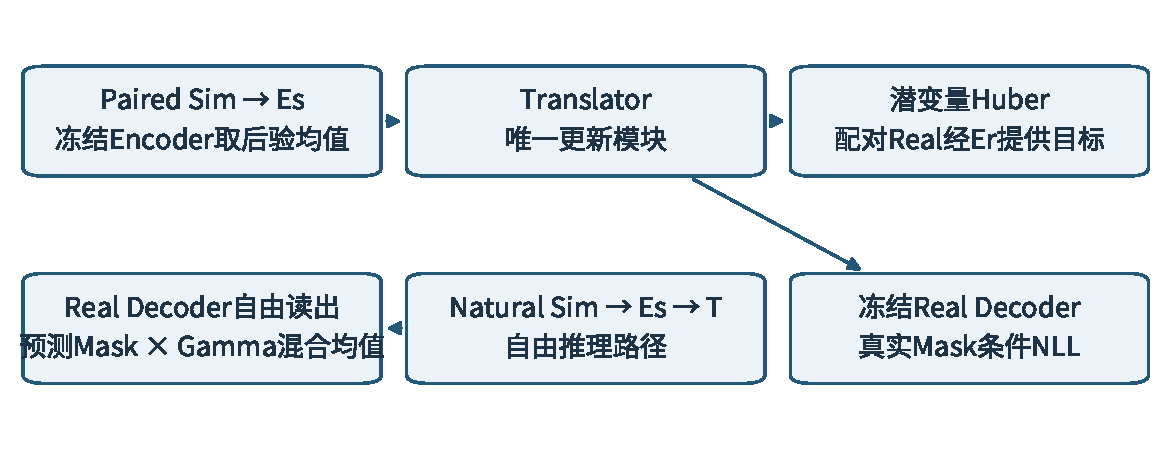
\includegraphics[width=0.97\textwidth]{figures/revision_20261127/ch05_translator_paths.pdf}
  \caption{伪配对监督训练与自由推理的数据流}
 \label{fig:ch05_translator_paths}
\end{figure}

算法\ref{alg:translator_training_and_decode}区分伪配对训练与自由推理；训练时冻结Decoder参数不阻断其对输入潜变量的梯度。
\begin{algorithm}[H]
\small
\caption{伪配对监督的潜变量映射与自由读出}\label{alg:translator_training_and_decode}
\KwIn{独立训练的两域VAE、训练伪配对及Natural Sim输入}
\KwOut{Translator参数与Real域风格触觉窗口}
冻结两域VAE参数，仅令Translator参数可更新\;
\ForEach{训练批次 $(X_s,X_r)$}{
计算后验均值 $Z_s=\mu_s(X_s)$、$Z_r=\mu_r(X_r)$\;
得到预测 $\widehat Z_r=T_\theta(Z_s)$\;
计算潜变量Huber损失\;
用真实前帧Mask作为循环上下文、真实当帧Mask作为幅值条件计算Decoder NLL\;
由Huber与$0.1$倍NLL之和反向传播，仅更新Translator\;
}
在规定候选轮次内依据验证目标选择检查点\;
\ForEach{部署输入 $X_s$}{
令 $Z_s=\mu_s(X_s)$，计算 $T_\theta(Z_s)$\;
Real Decoder依次使用BOS及预测前帧Mask，自回归生成当帧Mask\;
计算Gamma混合均值并恢复正值尺度，与预测Mask相乘\;
输出按原帧序组织的$4\times712$非负响应\;
}
\end{algorithm}
%



训练和验证分别使用1200与240个配对窗口。随机种子为4303，采用AdamW，学习率$3\times10^{-4}$、权重衰减$10^{-4}$，批量64，梯度范数上限5。每轮打乱训练窗口并执行19步，45轮共855步；在第30至45轮内按验证联合目标选择权重，最终采用第30轮，对应570次参数更新。末批包含48窗，验证时按各批样本数加权汇总，与训练采用相同的Huber和NLL组合，不依据域分类器分数挑选检查点。总训练步数与所存检查点经历的更新次数应分别记录。Natural Sim不直接参与该映射的配对训练。部署时仅需Natural输入，经Sim均值编码、Translator和Real Decoder生成完整触觉；Mask由模型预测，幅值取恢复尺度后的Gamma混合均值$s_{\rm pos}\sum_k\omega_k a_k/b_k$，无需Real样本、GMM或探针。

配对验证首先考察映射能否拟合所给监督，随后再检验其在自然任务输入上的输出质量。GMM责任度不是物理接触归属概率，Top-5分量筛选与单一候选选择压缩了多解信息，Translator未接收完整分量概率或候选分布。1200与240窗也不代表1440个独立Root。Paired Validation上，Translator与配对训练Real均值模板的潜变量Huber分别为0.32591983675956726和0.4942297637462616，按全部窗口、帧及潜维平均。该模板仅沿1200个配对训练目标的窗口维取均值，保留四帧位置，并广播至待评价窗口，不使用验证目标拟合。这一优势未覆盖全部Session，表明映射效果还受配对来源影响。Natural缺少同步Real目标，因此下一节将结合冻结评价器与结构指标，检验潜变量拟合改善能否延伸到712维输出。

% Independent section draft; no official main-file integration.
\section{跨域触觉重建实验结果与分析}
\label{sec:ch05_reconstruction_results}

为检验统计伪配对与双域表示是否支持完整触觉转换，本节采用迁移前训练并冻结的C0评价器。其由原Real Train与Natural Sim Train训练，包括Logistic、kNN及MLP、GRU、Transformer各Seed 11、12、13，共11个实例。权重、Scaler、log1p处理、通道顺序与0.5阈值保持不变，标签方向为Real=1、Sim=0。跨域评价比较780个Real Validation窗口与同划分905个Natural Sim窗口的转换结果，分别来自4个Session和10个Root。这些是开发验证数据，不是新独立盲测；后训练的Probe不能替代该协议。

\begin{figure}[htbp]
 \centering
 \fbox{\begin{minipage}{0.92\textwidth}\centering\small
 原Real Train与Natural Sim Train $\rightarrow$ 训练11个C0后冻结\\[3pt]
 Real Validation与Translated Natural Validation\\[3pt]
 $\downarrow$ 原log1p、Scaler及通道顺序\\[3pt]
 冻结C0、阈值0.5 $\rightarrow$ 逐实例BA、AUC、D及联合判定
 \par\vspace*{2.5mm}
 \end{minipage}}
 \caption{迁移前冻结C0的Validation评价协议}
 \label{fig:ch05_c0_validation_protocol}
\end{figure}

记两类召回率为$R_r$与$R_s$，则$\mathrm{BA}=(R_r+R_s)/2$，$D=1-2|\mathrm{BA}-0.5|$。每个实例必须同时满足BA在$[0.45,0.55]$、AUC在$[0.475,0.525]$及$D\ge0.90$，且11个实例全部满足才算联合通过。BA与D门槛数学等价，不是两项独立证据；AUC检验分数排序，不能在小于0.5时反转后参加验收。点估计按窗口计算，不应误称Session或Root等权宏平均。原始未转换数据上，11个C0的Validation BA均超过0.98，表明其已能区分原始两域；但冻结后的测试只覆盖这些模型学到的判别特征，即使通过也不能替代触觉结构与输入响应保持检查。

表\ref{tab:ch05_transfer_summary}汇总同角色跨域结果。C3采用原双域VAE与GRU Translator，其Validation结果取已有冻结链路复现，而非历史开发Test。虽然D全部达标，仅kNN同时满足AUC条件。表\ref{tab:ch05_validation_instances}中，C3的MLP分数仍保持正向排序差异，GRU和部分Transformer则出现反向排序；两种情况均不满足域不可辨识要求。例如MLP Seed11将905个迁移窗口全部判Real，Real中776/780判对，BA约0.497436；但AUC为0.591571。固定阈值下的高D因此可能来自类别预测偏向，不能证明分布已接近。

\begin{table}[htbp]
 \centering\small
 \caption{同划分Natural Validation的跨域评价汇总}
 \label{tab:ch05_transfer_summary}
 \begin{tabular}{lccc}
 \hline
 版本&目标域读出&BA/D及AUC联合&BA/D等价门槛\\\hline
 C3&原C3&1/11&11/11\\
 C13&幅值条件修复&1/11&11/11\\
 C27&原C3&2/11&11/11\\\hline
 \end{tabular}
\end{table}
\begin{table}[htbp]
 \centering\footnotesize
 \caption{C3与C27的冻结Validation逐实例结果}
 \label{tab:ch05_validation_instances}
 \begin{tabular}{lrrrrrr}
 \hline
 &\multicolumn{3}{c}{C3}&\multicolumn{3}{c}{C27}\\
 实例&BA&AUC&D&BA&AUC&D\\\hline
Logistic&0.498718&0.682604&0.997436&0.501480&0.673062&0.997039\\
kNN&0.501944&0.500536&0.996111&0.506364&0.509993&0.987272\\
MLP 11&0.497436&0.591571&0.994872&0.498541&0.600164&0.997082\\
MLP 12&0.498718&0.598765&0.997436&0.498718&0.630157&0.997436\\
MLP 13&0.498077&0.610894&0.996154&0.499734&0.617238&0.999469\\
GRU 11&0.498718&0.239559&0.997436&0.498718&0.571915&0.997436\\
GRU 12&0.498718&0.237257&0.997436&0.511978&0.487958&0.976045\\
GRU 13&0.498718&0.383622&0.997436&0.511425&0.548114&0.977150\\
Transformer 11&0.497436&0.282288&0.994872&0.497988&0.357940&0.995977\\
Transformer 12&0.496154&0.217189&0.992308&0.499469&0.307241&0.998938\\
Transformer 13&0.498077&0.698591&0.996154&0.503602&0.643598&0.992796\\
 \hline
 \end{tabular}
\end{table}

针对目标域读出，C13仅更新Real Decoder当前Mask条件嵌入和幅值头，冻结Encoder、Mask及循环骨干。同一Real验证集的重建MSE由0.07786883降至0.02631960，而Natural迁移联合结果仍为1/11，仅kNN通过。其MLP与Logistic的AUC仍高于上限，GRU与部分Transformer仍低于下限，说明局部幅值修复没有消除剩余可辨识特征。该现象不证明幅值无作用，只说明这一修复范围不足以完成整体转换。

C23进一步用原始Real与其C13重建输出作读出诊断，6/11满足同一数值门槛，包括Logistic、kNN、三个MLP及GRU Seed13；其余时序分类器未满足。该结果揭示目标域自重建仍存在可辨识痕迹，不是Natural迁移通过6/11。C24仅在相同幅值参数范围增加保留相邻帧的变化约束，同780个Real验证窗中，输出与Real的相邻保留帧log1p增量绝对误差由0.00281497降至0.00161364，但全窗全通道MSE升至0.02715745，汇总输出正值P99由3.54426降至3.28971，四帧总响应的跨窗标准差由67.58367降至57.52224；读出诊断仅kNN与Transformer Seed13满足，共2/11。时间统计改善与幅值尾部退化并存，不能将压低变化误差等同于更真实的触觉。Real帧间隔不均匀，该损失也不是物理时间导数。

C27保留原C3双域VAE，只适配Translator，增加Natural覆盖、Real坐标中的分布矩及源Patch响应份额约束，未混入C13 Decoder。新增通过GRU Seed12，使联合数由1增至2；但MLP、Logistic、GRU Seed11/13及三个Transformer仍未满足，且各实例AUC变化并非一致向0.5靠近。这支持有限适配带来局部变化，\mbox{不能}支持整体成功或稳定优势；D的11/11也不能覆盖其余九个实例的排序差异。

瓶颈证据指向监督与读出的共同限制，而非单纯未训练充分。配对状态复用、近Sim输入对应不同Real目标以及多解压缩提示监督歧义。Paired Train与Paired Validation中，19种放置后首帧指纹跨组复用，涉及后者97窗。指纹仅取九位小数精度的qpos与探针位置，不含速度等完整状态，不能等同于物理初态完全相同；但Real Session隔离也不能消除该复用风险。Natural又缺少对应Real真值，配对回归改善不能确认域外输入正确。加载与空间构型调整未解决全部配对覆盖，连续场、Taxel积分及处理诊断仅解释物理读出；这些都不是新的迁移成绩。扩散采样修复虽改善稳定性，仍未共同超过GRU的配对指标；直接OT和共享Encoder路线分别因坐标前提及结构保持停止，未执行的OT或C0不记为0/11。现有证据不能确定各因素的因果份额，也没有认证Taxel物理对应或真实任务收益。因而本章完成的是可追溯的重建与诊断链路，尚未完成完整域迁移验收。


% 第六、七章待后续授权写作；旧六章骨架保留，避免把总结误编号为第六章。
% % !TeX root = ../thesis.tex
\chapter{总结与展望}
\label{chap:ch06_conclusion}
% 正文待写：只允许使用已核实的研究材料。

\backmatter
\bibliographystyle{hithesis}
% 复用已核验参考文献库。
\bibliography{reference}
% 本科、硕士、博士后置顺序不同；当前不引入博士答辩决议/博士个人简历。
% 有真实内容后按学院要求启用：
% \begin{appendix}% !TeX root = ../thesis.tex
\chapter{待填写附录标题}
% 有实际附录材料时再加入。
\end{appendix}
% % !TeX root = ../thesis.tex
\begin{publication}
待核实并填写实际成果。没有成果时按学院要求处理，不使用示例虚构条目。
\end{publication}

% \authorization
% % !TeX root = ../thesis.tex
\begin{acknowledgements}
硕士阶段的学习与研究即将告一段落，谨向在此期间给予我指导、支持与帮助的老师、同学和家人致以诚挚的感谢。

首先，衷心感谢导师张展教授的指导。围绕灵巧手仿真、示教数据构建与触觉跨域重建开展研究的过程，使我逐步认识到，研究工作不仅需要实现方法，还需要明确问题、核实证据并审慎解释结果。导师的指导与要求，促使我不断检查研究思路和结论边界。这些训练将对我今后的学习与工作产生持续影响。

感谢哈尔滨工业大学计算学部提供的学习与研究环境，感谢学习和科研过程中与我交流、给予帮助的老师和同学。日常讨论使我能够从不同角度审视问题，也使研究中的困难与反复成为积累经验的过程。

感谢家人的理解与支持，使我能够专注于学业和研究。谨以此文向所有关心和帮助过我的人表达谢意。

\end{acknowledgements}

\end{document}
